\documentclass{AeroStructure-ERJohnson}

\allowdisplaybreaks

\usepackage{arydshln}

\input crosslink.tex

%\usepackage{showframe}
\def\ShowFrameLinethickness{0.125pt}

\def\harp#1{\smash{\mathord{\buildrel{\lower3pt\hbox{$\scriptscriptstyle\rightharpoonup$}}\over{#1}}}}

\myexternaldocument{App_4P}
\myexternaldocument{Ch01_4P}
\myexternaldocument{Ch02_4P}
\myexternaldocument{Ch03_4P}
\myexternaldocument{Ch04_4P}
\myexternaldocument{Ch05_4P}
\myexternaldocument{Ch06_4P}
\myexternaldocument{Ch07_4P}
\myexternaldocument{Ch08_4P}
\myexternaldocument{Ch09_4P}
\myexternaldocument{Ch10_4P}
\myexternaldocument{Ch11_4P}
\myexternaldocument{Ch12_4P}
\myexternaldocument{Ch13_4P}
\myexternaldocument{Ch14_4P}
\myexternaldocument{Ch15_4P}
\myexternaldocument{Ch16_4P}
\myexternaldocument{Ch17_4P}
%\myexternaldocument{Ch18_4P}

\begin{document}

\mainmatter

%\hbox{~}\clearpage
%\setcounter{page}{1}

\setcounter{chapter}{17}
\setcounter{page}{485}

\chapter{Introduction to flexible body~dynamics}

The transient response of a rocket at liftoff is presented to motivate the subject of structural dynamics. The accelerations at launch result in significant load factors imposed on the spacecraft, or payload. User guides for a launch vehicle specify load factors for preliminary design of the primary structure of the spacecraft. Often there are limits placed on the lowest natural frequency of the payload to ensure its dynamic characteristics do not adversely affect the control system of the booster (Sarafin, 1995). Thus, the capability to predict the load factor for the primary structure of the payload/spacecraft at launch, and the frequencies of the payload package, are necessary in the payload design. The example we begin with is the Atlas I.

\section{Description of Atlas I}\label{sec18.1}

A spacecraft consists of mission-specific equipment called the payload and a collection of subsystem components called a bus. Typical subsystem components may include attitude control, propulsion, communications, electrical power, etc. (Sarafin, 1995, p. 451). The spacecraft bus may be able to support different payloads for different missions. As shown in figure~\ref{fig18.1}, the main components of the Atlas I space launch vehicle from bottom to top are an expendable booster, an expendable second stage called Centaur, and the payload/spacecraft (Isakowitz, 1995). The spacecraft is covered by a fairing. An adapter, also known as a launch vehicle adapter, structurally links the spacecraft and Atlas I. The spacecraft developer usually designs the adapter.

Selected weights and thrust data for the Atlas I in table~\ref{tab18.1} are from Isakowitz (1995).

\begin{table}[h]%18.1
\processtable{Selected data for Atlas I\label{tab18.1}}{%
\tabcolsep=10pt\begin{tabular}{@{}ll@{}}
\toprule
Gross weight& 362,200 lb. \\
Booster weight& 321,100 lb. \\
Centaur (upper stage)& 34,300 lb. \\
Payload fairing& 3,027 lb \\
Payload& 3,773 lb \\
Engine thrust at liftoff& 439,300 lb. \\
\botrule
\end{tabular}}{}
\end{table}

{\def\thefigure{18.1}
\begin{sidewaysfigure}
\begin{center}
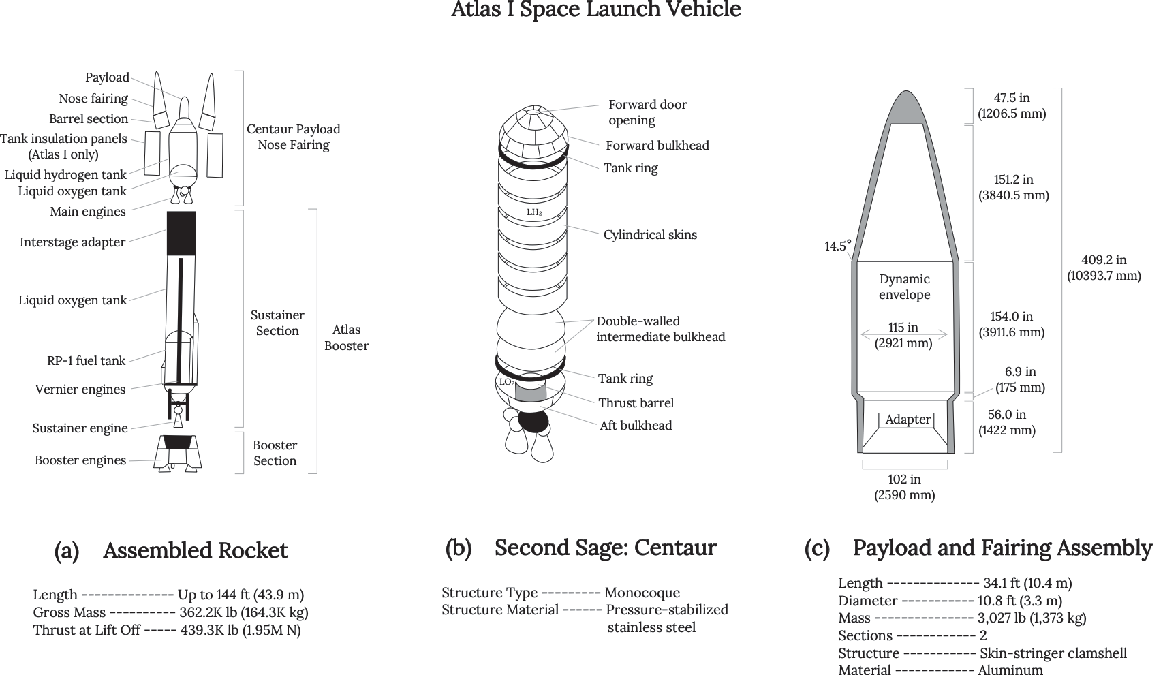
\includegraphics{Figure_18-1.pdf}
\caption{\label{fig18.1}}
\end{center}
\end{sidewaysfigure}
}




Propellant weights in the booster and second stage, and the approximate structural weight are listed in table~\ref{tab18.2}.

\begin{table}[h]%tab18.2
\vspace*{-0.6pc}
\processtable{Weights of propellants and structure for Atlas I\label{tab18.2}}{%
\begin{tabular}{@{}ll@{}}
\toprule
Booster propellant& 305,500 lb. \\
Centaur propellant& 30,000 lb. \\
Approximate structural weight$^{\rm a}$ & 22,927 lb.\\
\botrule
\end{tabular}}{\footnotesize
$^{\rm a}$Gross weight of 362,200 lb. less the sum of propellant weights of 335,500 lb. and the payload weight of 3,773 l.}
\vspace*{-1pc}
\end{table}

In terms of percentages
\begin{enumerate}\leftskip=12pt
  \item[] 92.6 percent of the total weight is propellant,
  \item[] 6.33 percent of the total weight is structure, and
  \item[] 1.04 percent of the total weight is payload.
\end{enumerate}

Clearly, most of the weight is propellant.

\subsubsection{Objective.} Determine the maximum vertical load factor of the payload at liftoff. We assume the loss of mass due to propellant burn-off is small and can be neglected in the initial instants after liftoff.

\section{Rigid body load factor}\label{sec18.2}
First, we assume Atlas I is a rigid body and determine the load factor from dynamic equilibrium. This analysis is shown in figure~\ref{fig18.2}, where it is determined that the load factor is 1.213. However, this rigid body analysis omits information on frequencies. To determine frequencies of the structure we must consider flexible body dynamics, which is discussed beginning in the next section.

{\def\thefigure{18.2}
\processfigure{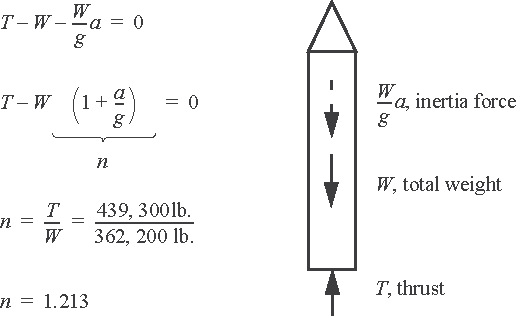
\includegraphics{Figure_18-2.pdf}
}{\caption{Rigid body analysis of Atlas I to determine the load factor at liftoff.\label{fig18.2}}}}

\pagebreak

\section{Steps in flexible body dynamics}\label{sec18.3}
\begin{enumerate}
  \item Equations of motion relative to the equilibrium state.
  \item Free vibration problem; normal modes.
  \item Coordinate transformation from physical coordinates to modal coordinates.
  \item Transform initial conditions from physical coordinates to modal coordinates. Solve for the time history of the modal coordinates.
  \item Transform back to physical coordinates.
  \item Calculate the payload acceleration time history.
\end{enumerate}

\subsubsection{Step 1: Equations of motion about equilibrium.}\label{step1} Consider a three-degree-of-freedom model of Atlas I shown in figure~\ref{fig18.3}(a). The model consists of three particles with lumped masses $m_1$, $m_2$, and $m_3$ and two springs with stiffnesses $k_{12}$, and $k_{23}$. Mass $m_1$ is one-half the mass of the booster and Centaur, mass $m_2$ is one-half of the mass of the booster and Centaur plus the mass of the fairing, and mass $m_3$ is the mass of the payload. The stiffness of the booster and Centaur is represented by $k_{12}$, and the stiffness of the launch vehicle adapter is represented by $k_{23}$.

{\def\thefigure{18.3}
\processfigure{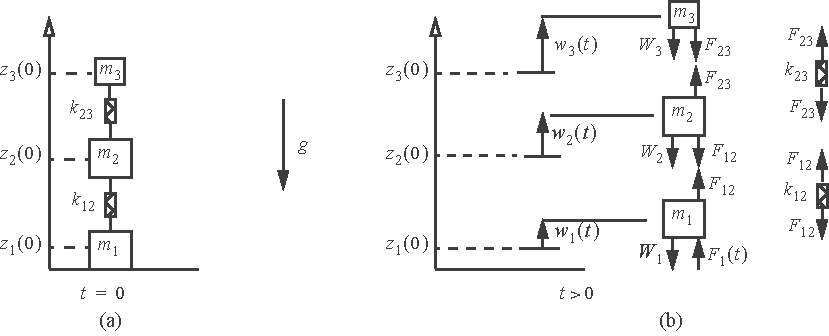
\includegraphics{Figure_18-3.pdf}
}{\caption{Three-degree-of-freedom model of Atlas I. (a) At rest. (b) Free body diagrams.\label{fig18.3}}}}

The axial coordinates of the particles in the equilibrium state at $t = 0$ are $z_{i}(0)$, $i=1,2,3$, and the displacements of the masses from their equilibrium state are denoted by $w_{i}(t)$, and $w_{i}(0)=0$. The weight of each particle is denoted by $W_{i}$, $i=1,2,3$. From the free body diagram shown in figure~\ref{fig18.3}(b) the equations of motion are
\begin{gather}
\label{eq18.1}
F_{1}(t)-W_{1}+F_{12}=m_{1} \ddot{w}_{1},\\
\label{eq18.2}
-W_{2}-F_{12}+F_{23}=m_{2} \ddot{w}_{2}, \text{and}\\
\label{eq18.3}
-W_{3}-F_{23}=m_{3} \ddot{w}_{3}.
\end{gather}
The two dots over the displacements is shorthand notation for the second derivative in time:
\begin{align}\label{eq18.4}
\ddot{w}_{i}(t)=\frac{d^{2} w_{i}}{d t^{2}}.
\end{align}
The spring forces are related to the relative coordinates between the particles. That is,
\begin{equation}\label{eq18.5}
\begin{split}
&F_{12}=k_{12}\left[\left(z_{2}(0)+w_{2}(t)\right)-\left(z_{1}(0)+w_{1}(t)\right)\right] \\
&F_{23}=k_{23}\left[\left(z_{3}(0)+w_{3}(t)\right)-\left(z_{2}(0)+w_{2}(t)\right)\right]
\end{split}.
\end{equation}
Substitute the spring force relations (\ref{eq18.5}) into the equations of motion (\ref{eq18.1}) to (\ref{eq18.3}) to get
\begin{gather}\label{eq18.6}
F_{1}(t)-W_{1}+k_{12}\left(z_{2}(0)-z_{1}(0)\right)=m_{1} \ddot{w}_{1}+k_{12} w_{1}-k_{12} w_{2},
\\\label{eq18.7}
-W_{2}-k_{12}\left(z_{2}(0)-z_{1}(0)\right)+k_{23}\left(z_{3}(0)-z_{2}(0)\right)=m_{2} \ddot{w}_{2}-k_{12} w_{1}+\left(k_{12}+k_{23}\right) w_{2}-k_{23} w_{3},\ \text{and}
\\\label{eq18.8}
-W_{3}-k_{23}\left(z_{3}(0)-z_{2}(0)\right)=m_{3} \ddot{w}_{3}-k_{23} w_{2}+k_{23} w_{3}.
\end{gather}
In the equilibrium state the eqs. (\ref{eq18.6}) to (\ref{eq18.8}) are
\begin{align}\label{eq18.9}
\begin{gathered}F_{1}(0)-W_{1}+k_{12}\left(z_{2}(0)-z_{1}(0)\right)=0 \\-W_{2}-k_{12}\left(z_{2}(0)-z_{1}(0)\right)+k_{23}\left(z_{3}(0)-z_{2}(0)\right) \\-W_{3}-k_{23}\left(z_{3}(0)-z_{2}(0)\right)\end{gathered}.
\end{align}
The solution of the equilibrium equation (\ref{eq18.9}) is
\begin{equation}\label{eq18.10}
\begin{split}
F_{1}(0)=W_{1}+W_{2}+W_{3}=362{,}200\,\mathrm{lb}. \\k_{23}\left[z_{3}(0)-z_{2}(0)\right]=-W_{3} \\k_{12}\left[z_{2}(0)-z_{1}(0)\right]=-W_{2}-W_{3}
\end{split}.
\end{equation}
Force $F_{1}(0)$ is the reaction force from the launch pad acting on the rocket in the equilibrium state prior to liftoff.


The equations of motion with respect to the equilibrium state are obtained by substituting eq.~(\ref{eq18.10}) into the equations of motion (\ref{eq18.6}) to (\ref{eq18.8}). Writing these equations in matrix form we get
\begin{align}\label{eq18.11}
\left[\begin{array}{@{}ccc@{}}m_{1} & 0 & 0 \\0 & m_{2} & 0 \\0 & 0 & m_{3}\end{array}\right]\left[\begin{array}{@{}c@{}}\ddot{w}_{1} \\\ddot{w}_{2} \\\ddot{w}_{3}\end{array}\right]+\left[\begin{array}{@{}ccc@{}}k_{12} & -k_{12} & 0 \\-k_{12} & k_{12}+k_{23} & -k_{23} \\0 & -k_{23} & k_{23}\end{array}\right]\left[\begin{array}{@{}l@{}}w_{1} \\w_{2} \\w_{3}\end{array}\right]=\left[\begin{array}{@{}c@{}}T(t) \\0 \\0\end{array}\right],
\end{align}
where the net thrust after liftoff is $T(t)=F_{1}(t)-F_{1}(0)$. Numerical evaluation for the masses of the particles are
\begin{gather*}
m_{1}=\frac{(321{,}100+34{,}300)}{2(32.2)}=5,518.63 \frac{1\mathrm{b} \cdot\!\mbox{-}\mathrm{s}^{2}}{\mathrm{ft}.},\quad  m_{2}=m_{1}+3,027/32.2=5,612.64 \frac{1\mathrm{b} \cdot\!\mbox{-}\mathrm{s}^{2}}{\mathrm{ft}.},\ \text{and}\\
m_{3}=3,773/32.2=117.17 \frac{1\mathrm{b} \cdot\!\mbox{-}\mathrm{s}^{2}}{\mathrm{ft}.}.
\end{gather*}
To estimate the structural stiffness of the booster and Centaur, assume the vehicle structure is a thin-walled cylindrical shell with a mean radius of 5 ft., and with an effective wall thickness $t_{w}$. We estimate the effective wall thickness in the following way: The approximate structural weight of the booster is 15,600 lb., and its length is 72.7 ft. The approximate weight of Centaur is 4,300 lb., and its length is 30 ft. We equate this structural weight to the volume of material in the shell wall of the booster and Centaur times the specific weight of stainless steel; i.e.,
\[
19{,}900\,\mathrm{lb}.=2 \pi(5\,\mathrm{ft}.) t_{w}(102.7\,\mathrm{ft}.)(12\,\mathrm{in}./\mathrm{ft}.)^{2} 0.286\,\mathrm{lb} {\cdot}/ \mathrm{in}.^{3}.
\]
Solve this equation for the booster shell wall thickness to get $t_{w}=0.149763\,\text{in}$. Hence the equivalent cross-sectional area of the booster and Centaur is $56.459\,\text{in.}^{2}$ The structural stiffness is given by
\[
k_{12}=\frac{E A}{L}=\frac{\left(28 \times 10^{6}\,\mathrm{lb}./\mathrm{in}.^{2}\right)\left(56.459\,\mathrm{in.}^{2}\right)}{(102.7\,\mathrm{ft}.)}=15.393 \times 10^{6}\,\mathrm{lb}./\mathrm{ft}.
\]
The estimate of the stiffness of the launch vehicle adapter is
\[
k_{23}=k_{12}/2=7.7014 \times 10^{6}\,\mathrm{lb}./\mathrm{ft}.
\]
We neglect the loss of mass due to fuel burn during the initial period of liftoff, and assume the net thrust is a step function of time. That is,
\[
T(t)=[439,300-362,200] H(t)=(77{,}100\,\mathrm{lb}.) H(t),
\]
where the unit step function $H(t)=0$ for $t<0,\text{ and }H(t)=1$ for $t>0$. Numerical evaluation of eq.~(\ref{eq18.11}) is
\begin{align}\label{eq18.12}
\left[\begin{array}{@{}ccc@{}}5,518.63 & 0 & 0 \\0 & 5,612.64 & 0 \\0 & 0 & 117.174\end{array}\right]\left[\begin{array}{@{}c@{}}\ddot{w}_{1} \\\ddot{w}_{2} \\\ddot{w}_{3}\end{array}\right]+10^{6}\left[\begin{array}{@{}ccc@{}}15.4027 & -15.4027 & 0 \\-15.4027 & 23.1041 & -7.70136 \\0 & -7.70136 & 7.70136\end{array}\right]\left[\begin{array}{@{}l@{}}w_{1} \\w_{2} \\w_{3}\end{array}\right]=\left[\begin{array}{@{}c@{}}76,100 \\0 \\0\end{array}\right].
\end{align}
The initial conditions for the rocket at rest are:
\begin{align}\label{eq18.13}
w_{i}(0)=0 \quad \dot{w}_{i}(0)=0 \quad i=1,2,3.
\end{align}
In compact notation the matrix equations of motion (\ref{eq18.12}) are
\begin{align}\label{eq18.14}
[M]\{\ddot{w}\}+[K]\{{w}\}=\{T\}.
\end{align}
The linear ordinary differential equation (\ref{eq18.14}) with constant coefficients can be solved numerically by step-by-step integration with respect to time, or they can be solved by the mode-separation method. The mode-separation method is limited to linear differential equations, but the step-by-step method can be used for linear and nonlinear ordinary differential equations. Step-by-step methods are discussed by Craig (1981, pp. 455--464) and Schiesser (1994), which contain many references to the literature. The mode-separation method is detailed in the following steps.

\subsubsection{Step 2: Free vibration problem.} For the free vibration problem set $\{T\}=0_{3 X 1}$, and seek a solution of the form
\begin{align}\label{eq18.15}
\{w(t)\}=\{\phi\} \cos (\omega t-\alpha).
\end{align}
Substitute eq.~(\ref{eq18.15}) into the free vibration equation of motion to get
\begin{align}\label{eq18.16}
\left([K]-\omega^{2}[M]\right)\{\phi\}(\cos \omega t-\alpha)=0 \quad \forall t>0.
\end{align}
Satisfying eq.~(\ref{eq18.16}) leads to
\begin{align}\label{eq18.17}
([K]-\lambda[M])\{\phi\}=0,\ \text{where}\ \lambda=\omega^{2}.
\end{align}
One solution to eq.~(\ref{eq18.17}) is for the amplitude vector $\{\phi\}=0_{3 X 1}$, which leads to $w(t)=0$ for all time. For non-zero solutions of the amplitude vector we require
\begin{align}\label{eq18.18}
\operatorname{Det}([K]-\lambda[M])=0.
\end{align}
Evaluating the determinate (\ref{eq18.18}) leads to the characteristic equation for $\lambda$, which in this case is a cubic polynomial:
\begin{align}\label{eq18.19}
\hspace*{6pt}\lambda\left[-k_{12} k_{23}\left(m_{1}+m_{2}+m_{3}\right)+\left(k_{12} m_{3}\left(m_{1}+m_{2}\right)+k_{23} m_{1}\left(m_{2}+m_{3}\right)\right) \lambda-m_{1} m_{2} m_{3} \lambda^{2}\right]=0.
\end{align}
Numerical solution for the roots of (\ref{eq18.19}), which are called eigenvalues, are
\begin{align}\label{eq18.20}
\lambda_{1}=67159.2 \quad \lambda_{2}=5474.23 \quad \lambda_{3}=0.
\end{align}
For each eigenvalue (\ref{eq18.20}) there are three linear equations to determine the amplitude vector $\{\phi\}$ obtained from eq.~(\ref{eq18.17}). Since the determinate of eq.~(\ref{eq18.17}) vanishes for each eigenvalue, the three linear equations to determine the amplitude vector $\{\phi\}$ corresponding to each $\lambda$ are not independent. Solutions for $\{\phi\}$ are called eigenvectors. From eigensystem software we find the following eigen pairs:
\begin{align}\label{eq18.21}
\left(\lambda_{1},\left\{\phi_{1}\right\}\right)=\left(67,159.2,\left[\begin{array}{@{}c@{}}0.945544 \times 10^{-3} \\-0.0218065 \\1\end{array}\right]\right),\ \left(\lambda_{2},\left\{\phi_{2}\right\}\right)=\left(5,474.23,\left[\begin{array}{@{}c@{}}-0.953559 \\0.916711 \\1\end{array}\right]\right), \& \left(\lambda_{3},\left\{\phi_{3}\right\}\right)=\left(0,\left[\begin{array}{@{}l@{}}1 \\1 \\1\end{array}\right]\right).
\end{align}
The eigen pairs $\left(\lambda_{1},\left\{\phi_{1}\right\}\right)$ and $\left(\lambda_{2},\left\{\phi_{2}\right\}\right)$ correspond to elastic modes, and $\left(\lambda_{3},\left\{\phi_{3}\right\}\right)$ corresponds to a rigid body mode. An eigenvector $\left\{\phi_{i}\right\}$ can be multiplied by a non-zero constant and still be a solution to eq.~(\ref{eq18.17}) with $\lambda=\lambda_{i}$.

\subsubsection{Step 3: Coordinate transformation.} Now consider the solution to the forced vibration problem (\ref{eq18.14}). Define the modal matrix $[\Phi]$ whose columns are the eigenvectors:
\begin{align}\label{eq18.22}
[\Phi]=\left[\left\{\phi_{1}\right\}\left\{\phi_{2}\right\}\left\{\phi_{3}\right\}\right]=\left[\begin{array}{@{}ccc@{}}0.945544 \times 10^{-3} & -0.953559 & 1 \\-0.0218065 & 0.916711 & 1 \\1 & 1 & 1\end{array}\right].
\end{align}
Transform from physical coordinates $\{w(t)\}$ to modal coordinates $\{q(t)\}$ using the modal matrix:
\begin{align}\label{eq18.23}
\left[\begin{array}{@{}l@{}}w_{1}(t) \\w_{2}(t) \\w_{3}(t)\end{array}\right]=[\Phi]\left[\begin{array}{@{}l@{}}q_{1}(t) \\q_{2}(t) \\q_{3}(t)\end{array}\right].
\end{align}

\subsubsection{Step 4: Solutions for the time history of modal coordinates.} Substitute transformation (\ref{eq18.23}) into the force vibration problem (\ref{eq18.14}) to get
\begin{align}\label{eq18.24}
[M][\Phi]\{\ddot{q}(t)\}+[K][\Phi]\{q(t)\}=\{T\}.
\end{align}
Pre-multiply the previous matrix equation by the transpose of the modal matrix and write the result as
\begin{align}\label{eq18.25}
\left[M_{g}\right]\{\ddot{q}(t)\}+\left[K_{g}\right]\{q(t)\}=\left\{T_{g}\right\}.
\end{align}
The generalized mass matrix is defined by $\left[M_{g}\right]=[\Phi]^{T}[M][\Phi]$, the generalized stiffness matrix by $\left[K_{g}\right]=[\Phi]^{T}[K][\Phi]$, and the generalized force vector by $\left\{T_{g}\right\}=[\Phi]^{T}\{T\}$. The generalized mass and stiffness \text{matrices} are diagonal matrices; that is, the off-diagonal elements in these matrices are zero and the diagonal elements are non-zero. Numerical results for these generalized matrices are
\begin{align}\label{eq18.26}
\left[M_{g}\right]=\left[\begin{array}{@{}ccc@{}}119.848 & 0 & 0 \\0 & 9,851.76 & 0 \\0 & 0 & 11,248.4\end{array}\right] \quad\left[K_{g}\right]=\left[\begin{array}{@{}ccc@{}}8.04888 \times 10^{6} & 0 & 0 \\0 & 5.39308 \times 10^{7} & 0 \\0 & 0 & 0\end{array}\right] \quad\left\{T_{g}\right\}=\left[\begin{array}{@{}c@{}}72.9014 \\-73,549.4 \\77,100\end{array}\right].
\end{align}
The equations of motion for the modal displacements are decoupled. Equations (\ref{eq18.13}) and (\ref{eq18.23}) determine the initial conditions for the modal displacements as
\[
\left[\begin{array}{@{}l@{}}q_{1}(0) \\q_{2}(t) \\q_{3}(t)\end{array}\right]=[\Phi]^{-1}\left[\begin{array}{@{}l@{}}w_{1}(0) \\w_{2}(0) \\w_{3}(0)\end{array}\right]\ \text{and}\ \left[\begin{array}{@{}l@{}}\dot{q}_{1}(0) \\\dot{q}_{2}(t) \\\dot{q}_{3}(t)\end{array}\right]=[\Phi]^{-1}\left[\begin{array}{@{}l@{}}\dot{w}_{1}(0) \\\dot{w}_{2}(0) \\\dot{w}_{3}(0)\end{array}\right]
\]
A convenient way to find the inverse of the modal matrix is to start with definition $[\Phi][\Phi]^{-1}=[I]$, pre-multiply it by $[\Phi]^{T}[M]$ to find $[\Phi]^{T}[M][\Phi][\Phi]^{-1}=[\Phi]^{T}[M]$. But $[\Phi]^{T}[K][\Phi]=\left[M_{g}\right]$. Hence,
\begin{align}\label{eq18.27}
[\Phi]^{-1}=\left[M_{g}\right]^{-1}[\Phi]^{T}[M].
\end{align}
The inverse of the generalized mass matrix is equal to the reciprocal of the diagonal elements of $\left[M_{g}\right]$. For this example the initial conditions for the modal coordinates are
\begin{align}\label{eq18.28}
q_{i}(0)=0 \quad \dot{q}_{i}(0)=0 \quad i=1,2,3.
\end{align}
The differential equation for the first modal displacement is
\begin{align}\label{eq18.29}
119.848 \ddot{q}_{1}+8.04888 \times 10^{6} q_{1}=72.9014 \quad q_{1}=q_{1}(t) \quad t \geq 0.
\end{align}
The solution to differential equation (\ref{eq18.29}) is
\begin{align}\label{eq18.30}
q_{1}(t)=9.05734 \times 10^{-6}+c_{2} \cos \omega_{1} t+c_{1} \sin \omega_{1} t,
\end{align}
where $\omega_{1}=\sqrt{\lambda_{1}}=259.151\,\mathrm{rad}/\mathrm{s}$. The constants $c_1$ and $c_2$ are determined from initial conditions (\ref{eq18.28}). The final result for the first modal displacement is
\begin{align}\label{eq18.31}
q_{1}(t)=9.05734 \times 10^{-6}\left(1-\cos \omega_{1} t\right) \quad \omega_{1}=259.151\,\mathrm{rad}/\mathrm{s}.
\end{align}
The differential equation for the second modal displacement is
\begin{align}\label{eq18.32}
9,851.76 \ddot{q}_{2}+5.39308 \times 10^{7} q_{2}=-73,549.4 \quad q_{2}=q_{2}(t) \quad t \geq 0.
\end{align}
The solution to differential equation (\ref{eq18.32}) subject to initial conditions (\ref{eq18.28}) is
\begin{align}\label{eq18.33}
q_{2}(t)=-0.00136322\left(1-\cos \omega_{2} t\right) \quad \omega_{2}=\sqrt{\lambda_{2}}=73.988\,\mathrm{rad}/\mathrm{s}.
\end{align}
The differential equation for the third modal displacement is
\begin{align}\label{eq18.34}
11,248.4 \ddot{q}_{3}=77,100 \quad q_{3}=q_{3}(t) \quad t \geq 0.
\end{align}
The solution to differential equation (\ref{eq18.34}) subject to initial conditions (\ref{eq18.28}) is
\begin{align}\label{eq18.35}
q_{3}(t)=3.42714 t^{2}.
\end{align}

\subsubsection{Step 5: Transform back to physical coordinates.} Equations (\ref{eq18.30}), (\ref{eq18.33}), and (\ref{eq18.35}) are substituted for $q_1$, $q_2$. and $q_3$, respectively, into the transformation (\ref{eq18.23}) to determine the physical displacements. The payload displacement is
\begin{align}\label{eq18.36}
w_{3}(t)=-0.00135416+3.42714 t^{2}+0.00136322 \cos (73.988 t)-9.05734 \times 10^{-6} \cos (259.151 t).
\end{align}

\subsubsection{Step 6: Payload acceleration.} The payload acceleration computed from the second derivative of eq.~(\ref{eq18.36}) is
\begin{align}\label{eq18.37}
\ddot{w}_{3}(t)=6.85428-7.46257 \cos (73.988 t)+0.608283 \cos (259.151 t).
\end{align}
The payload acceleration over one period of the lowest frequency is plotted in figure~\ref{fig18.4}. Maximum acceleration is $14.56\,\mathrm{ft}./\mathrm{s}^{2}$ at $t=0.0453\,\mathrm{s}$. The payload load factor is $n=1+14.56/32.2=1.452$, which is a 19.7 percent increase with respect to the rigid body load factor.

{\def\thefigure{18.4}
\processfigure{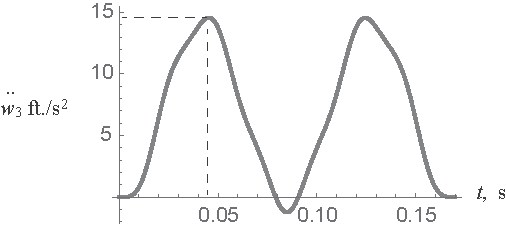
\includegraphics{Figure_18-4.pdf}
}{\caption{Time history of the
payload acceleration.\label{fig18.4}}}}

\vspace*{-1pc}

\section{Eigenvalue problems for real symmetric matrices}\label{sec18.4}

In general an \textit{nxn} real matrix $[A]$ acts on an \textit{nx1} vector $\{\phi\}$ by changing both its magnitude and direction. For example consider
\begin{align}\label{18.4a}
[A]=\left[\begin{array}{@{}ll@{}}2 & 1 \\1 & 2\end{array}\right] \quad\{\phi\}=\left[\begin{array}{@{}l@{}}2 \\0\end{array}\right] \quad[A]\{\phi\}=\left[\begin{array}{@{}l@{}}4 \\2\end{array}\right].\tag{a}
\end{align}
Vectors $\{\phi\}$ and $[A]\{\phi\}$ are depicted in figure~\ref{fig18.5}(a). Matrix $[A]$ may act on certain vectors by changing only their magnitude, and leaving their direction unchanged; e.g.,
\begin{align}\label{18.4b}
\left[\begin{array}{@{}ll@{}}2 & 1 \\1 & 2\end{array}\right]\left[\begin{array}{@{}l@{}} 1\\1\end{array}\right]=\left[\begin{array}{@{}l@{}}3 \\3\end{array}\right]=3\left[\begin{array}{@{}l@{}}1 \\1\end{array}\right].\tag{b}
\end{align}
Vector $\left[\begin{array}{@{}ll@{}}1 & 1\end{array}\right]^{T}$ is an eigenvector of matrix $[A]$ and the number ``3'' is an eigenvalue. Consider the vector $\left[\begin{array}{@{}ll@{}}-1 & 1\end{array}\right]^{T}$. Then, the matrix $[A]$ operating on this second vector is
\begin{align}\label{18.4c}
\left[\begin{array}{@{}ll@{}}2 & 1 \\1 & 2\end{array}\right]\left[\begin{array}{@{}c@{}}-1 \\1\end{array}\right]=\left[\begin{array}{@{}c@{}}-1 \\1\end{array}\right].\tag{c}
\end{align}
Thus, vector $\left[\begin{array}{@{}ll@{}}-1 & 1\end{array}\right]^{T}$ is an eigenvector and the number ``1'' is the eigenvalue. The eigenvectors of matrix $[A]$ are depicted in figure~\ref{fig18.5}(b).

{\def\thefigure{18.5}
\processfigure{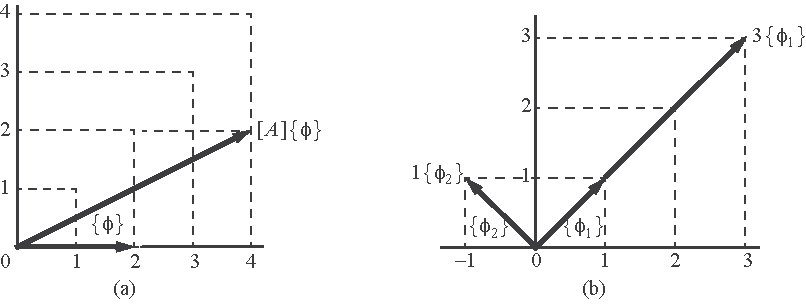
\includegraphics{Figure_18-5.pdf}
}{\caption{(a) Matrix A operating on a vector. (b) Matrix A operating on eigenvectors\label{fig18.5}}}}

\pagebreak

The eigenpairs of matrix $[A]$ are written as
\begin{align}\label{18.4d}
\left(\lambda_{1},\left\{\phi_{1}\right\}\right)=\left(3,\left[\begin{array}{@{}l@{}}1 \\1\end{array}\right]\right) \quad \text{and } \quad\left(\lambda_{2},\left\{\phi_{2}\right\}\right)=\left(1,\left[\begin{array}{@{}c@{}}-1 \\1\end{array}\right]\right).\tag{d}
\end{align}

\vspace*{-1pc}

The standard matrix eigenvalue problem is
\begin{align}\label{eq18.38}
[A]\{\phi\}=\lambda\{\phi\},
\end{align}
where $[A]$ is a real \textit{nxn} matrix and $\{\phi\}$ is an \textit{nx1 }vector. It is also written as
\begin{align}\label{18.4e}
([A]-\lambda[I])\{\phi\}=0.\tag{e}
\end{align}
where $[I]$ is the \textit{nxn} identity matrix. (i.e., a diagonal matrix with each diagonal element equal to one). One solution to eq.~(\ref{eq18.38}) is $\{\phi\}=0_{n X 1}$, which is called the trivial solution. Non-trivial solutions for $\{\phi\}$ require
\begin{align}\label{eq18.39}
\operatorname{\it Det}([A]-\lambda[I])=p(\lambda)=0,
\end{align}
where $p(\lambda)$ is a polynomial of degree $n$ having $n$ roots. The polynomial $p(\lambda)$ is called the characteristic equation. The roots of $p(\lambda)=0$ are the eigenvalues of matrix $[A]$. The eigenvalue problem for the \textit{r-th} mode is
\begin{align}\label{eq18.40}
[A]\left\{\phi_{r}\right\}=\lambda_{r}\left\{\phi_{r}\right\}.
\end{align}
The eigenpairs are denoted by $\left(\lambda_{r},\left\{\phi_{r}\right\}\right)$. If $\left\{\phi_{r}\right\}$ is a solution to eq.~(\ref{eq18.40})), then $c_{r}\left\{\phi_{r}\right\}$ is also a solution where $c_{r}$ is an arbitrary constant. Thus, the solution for the eigenvector is not unique. Scaling, or normalization, is the process to make the amplitude of the eigenvector unique. One method to normalize the amplitude is to require $\left\{\phi_{r}\right\}$ be a unit vector in the $n$-dimensional space. That is, we specify
\begin{align}\label{eq18.41}
\left\{\phi_{r}\right\}^{T}\left\{\phi_{r}\right\}=1.
\end{align}
Consider the eigenvalue problem for \textit{s-th} mode
\begin{align}\label{eq18.42}
[A]\left\{\phi_{s}\right\}=\lambda_{s}\left\{\phi_{s}\right\}.
\end{align}

\vspace*{-1pc}\pagebreak

\noindent Pre-multiply the \textit{r-th} mode in eq.~(\ref{eq18.40}) by $\left\{\phi_{s}\right\}^{T}$ to get
\begin{align}\label{eq18.43}
\left\{\phi_{s}\right\}^{T}[A]\left\{\phi_{r}\right\}=\lambda_{r}\left\{\phi_{s}\right\}^{T}\left\{\phi_{r}\right\}.
\end{align}
Pre-multiply the \textit{s-th} mode in eq.~(\ref{eq18.42}) by $\left\{\phi_{r}\right\}^{T}$:
\begin{align}\label{eq18.44}
\left\{\phi_{r}\right\}^{T}[A]\left\{\phi_{s}\right\}=\lambda_{s}\left\{\phi_{r}\right\}^{T}\left\{\phi_{s}\right\}.
\end{align}
Take the transpose of eq.~(\ref{eq18.43}) and use the property of symmetry $[A]^{T}=[A]$ to find
\begin{align}\label{eq18.45}
\left\{\phi_{r}\right\}^{T}[A]\left\{\phi_{s}\right\}=\lambda_{r}\left\{\phi_{r}\right\}^{T}\left\{\phi_{s}\right\}.
\end{align}
Subtract eq.~(\ref{eq18.45}) from eq.~(\ref{eq18.44}) to find
\begin{align}\label{eq18.46}
0=\left(\lambda_{r}-\lambda_{s}\right)\left\{\phi_{r}\right\}^{T}\left\{\phi_{s}\right\}.
\end{align}
For $\lambda_{r} \neq \lambda_{s}$
\begin{align}\label{eq18.47}
\left\{\phi_{r}\right\}^{T}\left\{\phi_{s}\right\}=0 \quad r \neq s \quad r, s=1,2, \ldots, n.
\end{align}
The eigenvectors for distinct eigenvalues are orthogonal. The eigenvectors are said to be orthonormal if
\begin{align}\label{eq18.48}
\left\{\phi_{r}\right\}^{T}\left\{\phi_{s}\right\}= \begin{cases}1 & r=s \\ 0 & r \neq s\end{cases}.
\end{align}

\vspace*{-1pc}

Since the characteristic equation $p(\lambda)=0$ has real coefficients, the roots $\lambda$ are real or occur as complex conjugate pairs. It can be shown that roots are real (Boresi, 1965, p. 34).

Let $[\Phi]$ denote the \textit{nxn} modal matrix whose columns are the orthonormal eigenvectors. The $r$-th column contains the eigenvector $\left\{\phi_{r}\right\}$ associated with eigenvalue $\lambda_{r}$, $r=1,2, \ldots, n$. Since the eigenvectors are orthonormal, the modal matrix has the property
\begin{align}\label{eq18.49}
[\Phi]^{T}[\Phi]=[\Phi][\Phi]^{T}=[I].
\end{align}
The modal matrix is called an \textbf{orthogonal matrix}, and it has the properties
\begin{align}\label{eq18.50}
[\Phi]^{-1}=[\Phi]^{T} \quad \operatorname{\it Det}[\Phi]=1.
\end{align}
Using the modal matrix the standard eigenvalue problem can be written as
\begin{align}\label{eq18.51}
[A][\Phi]=[\Phi][D],
\end{align}
where $[D]$ is a diagonal matrix of the eigenvalues:
\begin{align}\label{eq18.52}
[D]=\operatorname{diag}\left[\lambda_{1}, \lambda_{2}, \ldots, \lambda_{n}\right].
\end{align}
Post-multiply eq.~(\ref{eq18.51}) by $[\Phi]^{T}$ to get
\begin{align}\label{eq18.53}
[A] \underbrace{[\Phi][\Phi]^{T}}_{[I]}=[\Phi][D][\Phi]^{T}.
\end{align}
Hence, matrix $[A]$ has the decomposition
\begin{align}\label{eq18.54}
[A]=[\Phi][D][\Phi]^{T}.
\end{align}
\indent An \textit{nxn} real, symmetric matrix is \textbf{positive definite} if all eigenvalues $\lambda_{r}>0$, $r=1,2, \ldots, n$. It is \textbf{positive} \textbf{semidefinite} if the eigenvalues $\lambda_{r} \geq 0$, that is, some of its eigenvalues may equal zero. For structures having rigid body freedoms the stiffness matrix \textit{[K]} has as many zero eigenvalues as it has rigid body modes.

The mode superposition method leads to the generalized eigenvalue problem
\begin{align}\label{eq18.55}
[K]\{\phi\}=\lambda[M]\{\phi\},
\end{align}
where the \textit{nxn} matrices \textit{[K]} and \textit{[M]} are real and symmetric, $\{\phi\}$ is the \textit{nx1} eigenvector, or modal vector, and the eigenvalue $\lambda$ is equal to the square of the natural frequency $\omega$. Refer to eq.~(\ref{eq18.17}). The generalized eigenvalue problem (\ref{eq18.55}) can be reduced to the standard form in eq.~(\ref{eq18.38}) if the mass matrix is positive definite (Bathe, p. 573). Then all the properties of the eigenvalues, eigenvectors, and characteristic polynomials can be derived from the properties of the standard eigenvalue problem. In particular, for the generalized eigenvalue problem
\begin{itemize}
  \item all $n$ of the $\lambda_{r}$'s are real (no complex conjugates), and
  \item for $r \neq s$, $\left\{\phi_{r}\right\}^{T}[M]\left\{\phi_{s}\right\}=0$ (i.e., the eigenvectors are \textit{M}-orthogonal).
\end{itemize}

Vanishing of the determinate $\operatorname{\it Det}([K]-\lambda[M])=p(\lambda)=0$ is equivalent to finding the roots of a polynomial of degree $n$. If $n \geq 5$, iterative solution procedures have to be employed (Graig, 1981). There are many efficient subroutines available in various scientific subroutine libraries to numerically solve eigenvalue problems. In \textit{Mathematica} the function ``Eigensystem[{K,M}]'' finds numerical eigenvalues and eigenvectors of the generalized eigenvalue problem. In MATLAB the statement ``[V,D] = EIG(K,M)'' finds a diagonal matrix D of generalized eigenvalues and a full matrix V whose columns are the corresponding eigenvectors so that $[K][V]=[M][V][D]$. For the numerical solutions to the practice exercises listed in article \ref{sec18.11} it is assumed the reader has access to a subroutine to find eigenvalues and eigenvectors.

{\def\thefigure{18.6}
\processfigure[b]{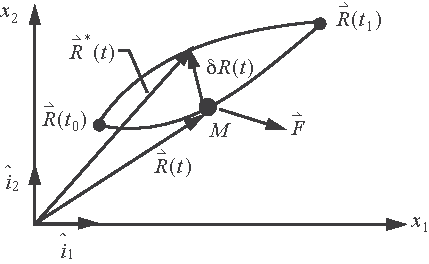
\includegraphics{Figure_18-6.pdf}
}{\caption{Dynamical paths for a
particle in plane motion.\label{fig18.6}}}}

\section{Hamilton's principle and Lagrange's equations}\label{sec18.5}

Consider a particle of mass \textit{M} in motion along the $x_1$-$x_2$ plane as shown in figure~\ref{fig18.6}. The position vector of the particle at time $t$ is denoted by $\harp{R}(t)$, where
\begin{align}\label{eq18.56}
\harp{R}(t)=x_{1}(t) \hat{i}_{1}+x_{2}(t) \hat{i}_{2},
\end{align}
where $\hat{i}_{1}$ and $\hat{i}_{2}$ are unit vectors in the $x_{1}$-, and $x_2$-directions, respectively. From Newton's second law the equation of motion for the particle is solved for its motion $\harp{R}(t)$, $t>t_{0}$, given its position $\harp{R}\left(t_{0}\right)$ and the velocity $\frac{d \harp{R}}{d t}\left(t_{0}\right)$ at $t=t_{0}$. In contrast to Newton's method, Hamilton's approach to this moving particle is to determine the motion $\harp{R}(t)$ given the positions $\harp{R}\left(t_{0}\right)$ and $\harp{R}\left(t_{1}\right)$, $t_{1}>t_{0}$. All positions in the interval $t_{0} \leq t \leq t_{1}$ describe a time-dependent path illustrated by a curve in figure~\ref{fig18.6}. The path labeled $\harp{R}(t)$ represents the actual motion. The path labeled $\harp{R}^{*}(t)$~represents a motion from $\harp{R}\left(t_{0}\right)$ to $\harp{R}\left(t_{1}\right)$ in the vicinity of the actual motion.



Begin with D'Alembert's principle and introduce the inertia force in addition the applied force $\harp{F}$ and write the dynamic equation of equilibrium as follows:
\begin{align}\label{eq18.57}
\harp{F}-M \frac{d^{2} \harp{R}}{d t^{2}}=0.
\end{align}
At a \textit{fixed} time introduce an infinitesimal virtual displacement denoted by the function $\delta \harp{R}(t)$. We can imagine the motion is stopped at time $t$ when the virtual displacement is imposed on the particle with both the applied force and inertia force acting on the particle. The virtual changes in the coordinates imposed on the particle at a fixed time are denoted by $\delta x_{1}(t)$ and $\delta x_{2}(t)$, so that
\begin{align}\label{eq18.58}
\delta \harp{R}(t)=\delta x_{1}(t) \hat{i}_{1}+\delta x_{2}(t) \hat{i}_{2}.
\end{align}
The varied path $\harp{R}^{*}(t)$ in the vicinity of the actual path $\harp{R}(t)$ is
\begin{align}\label{eq18.59}
\harp{R}^{*}(t)=\harp{R}(t)+\delta \harp{R}(t).
\end{align}
Since the varied path and actual path coincide at $t = t_0$ and $t=t_1$ the virtual displacement vanishes at these times:
\begin{align}\label{eq18.60}
\delta \harp{R}\left(t_{0}\right)=\delta \harp{R}\left(t_{1}\right)=0 \hat{i}_{1}+0 \hat{i}_{2}.
\end{align}
The virtual work of the applied force and the inertia force acting through the virtual displacement is given by the scalar product of eq.~(\ref{eq18.57}) with the virtual displacement in eq.~(\ref{eq18.58}):
\begin{align}\label{eq18.61}
\harp{F} \bullet \delta \harp{R}-M \frac{d^{2} \harp{R}}{d t^{2}} \bullet \delta \harp{R}=0.
\end{align}
Consider the relation
\begin{align}\label{eq18.62}
\frac{d}{d t}\left(\frac{d \harp{R}}{d t} \bullet \delta \harp{R}\right)=\frac{d^{2} \harp{R}}{d t^{2}} \bullet \delta \harp{R}+\frac{d \harp{R}}{d t} \bullet \frac{d}{d t}(\delta \harp{R}).
\end{align}
The virtual change in velocity is defined by
\begin{align}\label{eq18.63}
\delta\left(\frac{d \harp{R}}{d t}\right) \equiv \frac{d \harp{R}^{*}}{d t}-\frac{d \harp{R}}{d t}=\frac{d}{d t}\left(\harp{R}^{*}-\harp{R}\right)=\frac{d}{d t}(\delta \harp{R}).
\end{align}
Equation (\ref{eq18.63}) shows we can interchange the virtual operator $\delta(\quad)$ and the differential operator $d(\quad)/d t$. Use the result from eq.~(\ref{eq18.63}) to write eq.~(\ref{eq18.62}) as
\begin{align}\label{eq18.64}
\frac{d}{d t}\left(\frac{d \harp{R}}{d t} \bullet \delta \harp{R}\right)=\frac{d^{2} \harp{R}}{d t^{2}} \bullet \delta \harp{R}+\frac{d \harp{R}}{d t} \bullet \delta\left(\frac{d \harp{R}}{d t}\right).
\end{align}
Equation (\ref{eq18.64}) is incorporated into the virtual work eq.~(\ref{eq18.61}) to get
\begin{align}\label{eq18.65}
\harp{F} \bullet \delta \harp{R}+M \frac{d \harp{R}}{d t} \bullet \delta\left(\frac{d \harp{R}}{d t}\right)-\frac{d}{d t}\left(M \frac{d \harp{R}}{d t} \bullet \delta \harp{R}\right)=0.
\end{align}
The virtual work of the applied force is written as $\delta W=\harp{F} \bullet \delta \harp{R}$, and let the velocity of the particle be denoted by $\harp{v}=\frac{d \harp{R}}{d t}$, and its virtual velocity by $\delta \harp{v}=\delta\left(\frac{d \harp{R}}{d t}\right)$. Then, eq.~(\ref{eq18.65}) for the virtual work is
\begin{align}\label{eq18.66}
\delta W+M \harp{\nu} \bullet \delta \harp{\nu}-\frac{d}{d t}(M \harp{\nu} \bullet \delta \harp{R})=0.
\end{align}
The kinetic energy of the particle is $T=\frac{1}{2} M \harp{\nu} \bullet \harp{\nu}$, and its kinetic energy on the varied path is
\begin{align}\label{eq18.67}
T+\Delta T=\frac{1}{2} M(\harp{\nu}+\delta \harp{\nu}) \bullet(\harp{\nu}+\delta \harp{\nu})=\underbrace{\frac{1}{2} M \harp{\nu} \bullet \harp{\nu}}_{T}+\underbrace{M \harp{\nu} \bullet \delta \harp{\nu}}_{\delta T}+\underbrace{\frac{1}{2} M \delta \harp{\nu} \bullet \delta \harp{\nu}}_{\delta^{2} T}.
\end{align}
For infinitesimal virtual velocities $\Delta T \approx \delta T$. Integrate eq.~(\ref{eq18.66}) with respect to time from $t_0$ to $t_1$ to get
\begin{align}\label{eq18.68}
\int_{t_{0}}^{t_{1}}(\delta W+\delta T) d t-(M \harp{v} \cdot \delta \harp{R})\Big|_{t_{0}} ^{t_{1}}=0.
\end{align}
The virtual displacement $\delta \harp{R}$ vanishes at times $t_0$ and $t_1$. Then eq.~(\ref{eq18.68}) becomes
\begin{align}\label{eq18.69}
\int_{t_{0}}^{t_{1}}(\delta W+\delta T) d t=0.
\end{align}
Equation (\ref{eq18.69}) is Hamilton's principle. Note that $\delta W$ is not the total virtual work. It is the virtual work of the non-inertial forces.


\subsection{Lagrange's equations}\label{sec18.5.1}
Deriving equations of motion for connected bodies using Newton's laws as was done in step 1 of article \ref{sec18.3} requires separate free body diagrams of each component, and the forces of interaction had to be eliminated to arrive at the final set of equations. An alternative method is to use the scalar functions kinetic energy \textit{T} and the potential energy \textit{V} of the system in Lagrange's equations to obtain the equations of motion. Lagrange's equations are derived from Hamilton's variational principle (\ref{eq18.69}). In general, the kinetic energy of a particle as depicted in figure~\ref{fig18.6} is a function of its position ($x_1$, $x_2$) and its velocities $\left(\dot{x}_{1}, \dot{x}_{2}\right)$ at time $t$ (i.e., $T=T\left(x_{1}, x_{2}, \dot{x}_{1}, \dot{x}_{2}\right)$). The virtual change in kinetic energy is
\begin{align}\label{eq18.70}
\delta T=\frac{\partial T}{\partial x_{1}} \delta x_{1}+\frac{\partial T}{\partial x_{2}} \delta x_{2}+\frac{\partial T}{\partial \dot{x}_{1}} \delta \dot{x}_{1}+\frac{\partial T}{\partial \dot{x}_{2}} \delta \dot{x}_{2}.
\end{align}

\vspace*{-1pc}

The virtual work of the applied force acting on the particle is $\delta W=\harp{F} \bullet \delta \harp{R}=F_{1} \delta x_{1}+F_{2} \delta x_{2}$. The applied forces can be decomposed as $F_{i}=Q_{i}+R_{i}$, $i=1,2$, where $Q_{i}$ are non-conservative forces and $R_{i}$ are the conservative forces. Conservative forces are determined in terms of the potential energy function $V\left(x_{1}, x_{2}\right)$ by the relations
\begin{align}\label{eq18.71}
R_{1}=-\left(\frac{\partial V}{\partial x_{1}}\right) \quad R_{2}=-\left(\frac{\partial V}{\partial x_{2}}\right).
\end{align}

\vspace*{-1pc}\pagebreak

\noindent The virtual work is expressed as
\begin{align}\label{eq18.72}
\delta W=\left(Q_{1}+R_{1}\right) \delta x_{1}+\left(Q_{2}+R_{2}\right) \delta x_{2}=\left(Q_{1}-\frac{\partial V}{\partial x_{1}}\right) \delta x_{1}+\left(Q_{2}-\frac{\partial V}{\partial x_{2}}\right) \delta x_{2}.
\end{align}

\vspace*{-1.4pc}

Substitue the virtual kinetic energy from eq.~(\ref{eq18.70}) and the virtual work from eq.~(\ref{eq18.72}) into Hamilton's principle (\ref{eq18.69}) to get
\begin{align}\label{eq18.73}
\int_{t_0}^{t_1}\left[\left(Q_{1}-\frac{\partial V}{\partial x_{1}}\right) \delta x_{1}+\left(Q_{2}-\frac{\partial V}{\partial x_{2}}\right) \delta x_{2}+\frac{\partial T}{\partial x_{1}} \delta x_{1}+\frac{\partial T}{\partial x_{2}} \delta x_{2}+\frac{\partial T}{\partial \dot{x}_{1}} \delta \dot{x}_{1}+\frac{\partial T}{\partial \dot{x}_{2}} \delta \dot{x}_{2}\right] d t=0.
\end{align}
Rearrange the terms in eq.~(\ref{eq18.73}) to
\begin{align}\label{eq18.74}
\int_{t_0}^{t_1}\left[\left(Q_{1}-\frac{\partial V}{\partial x_{1}}+\frac{\partial T}{\partial x_{1}}\right) \delta x_{1}+\left(Q_{2}-\frac{\partial V}{\partial x_{2}}+\frac{\partial T}{\partial x_{2}}\right) \delta x_{2}+\frac{\partial T}{\partial \dot{x}_{1}} \delta \dot{x}_{1}+\frac{\partial T}{\partial \dot{x}_{2}} \delta \dot{x}_{2}\right] d t=0.
\end{align}
Integrate by parts the last two terms in the integrand of eq.~(\ref{eq18.74}) and note that the virtual coordinates $\delta x_{1}$ and $\delta x_{2}$ vanish at the beginning and end time. Hence, eq.~(\ref{eq18.74}) becomes
\begin{align}\label{eq18.75}
\int_{t_{0}}^{t_{1}}\left(\frac{\partial T}{\partial \dot{x}_{1}} \delta \dot{x}_{1}+\frac{\partial T}{\partial \dot{x}_{2}} \delta \dot{x}_{2}\right) d t=\int_{t_{0}}^{t_{1}}\left[-\frac{d}{d t}\left(\frac{\partial T}{\partial \dot{x}_{1}}\right)-\frac{d}{d t}\left(\frac{\partial T}{\partial \dot{x}_{2}}\right)\right] d t+\underbrace{\left.\left[\left(\frac{\partial T}{\partial \dot{x}_{1}}\right) \delta x_{1}+\left(\frac{\partial T}{\partial \dot{x}_{2}}\right) \delta x_{2}\right]\right|_{t_{0}} ^{t_{1}}}_{=0}.
\end{align}
The result of the manipulations from eq.~(\ref{eq18.73})to eq.~(\ref{eq18.75}) is
\begin{align}\label{eq18.76}
\int_{t_0}^{t_1}\left[\left(Q_{1}-\frac{\partial V}{\partial x_{1}}+\frac{\partial T}{\partial x_{1}}-\frac{d}{d t}\left(\frac{\partial T}{\partial \dot{x}_{1}}\right)\right) \delta x_{1}+\left(Q_{2}-\frac{\partial V}{\partial x_{2}}+\frac{\partial T}{\partial x_{2}}-\frac{d}{d t}\left(\frac{\partial T}{\partial \dot{x}_{2}}\right)\right) \delta x_{2}\right] d t=0.
\end{align}
Define the Lagranian function \textit{L} by
\begin{align}\label{eq18.77}
L=T-V.
\end{align}
Incorporating the Lagranian function in eq.~(\ref{eq18.76}) we get
\begin{align}\label{eq18.78}
\int_{t_{0}}^{t_{1}}\left[\left(Q_{1}+\frac{\partial L}{\partial x_{1}}-\frac{d}{d t}\left(\frac{\partial L}{\partial \dot{x}_{1}}\right)\right) \delta x_{1}+\left(Q_{2}+\frac{\partial L}{\partial x_{2}}-\frac{d}{d t}\left(\frac{\partial L}{\partial \dot{x}_{2}}\right)\right) \delta x_{2}\right] d t=0.
\end{align}
Equation (\ref{eq18.78}) vanishes for every choice of the virtual coordinates $\delta x_{1}$ and $\delta x_{2}$, which leads to Lagrange's equations of motion given by eq.~(\ref{eq18.79}) below.
\begin{align}\label{eq18.79}
\frac{d}{d t}\left(\frac{\partial L}{\partial \dot{x}_{1}}\right)-\frac{\partial L}{\partial x_{1}}=Q_{1} \quad \frac{d}{d t}\left(\frac{\partial L}{\partial \dot{x}_{2}}\right)-\frac{\partial L}{\partial x_{2}}=Q_{2}.
\end{align}

\vspace*{-1pc}

\begin{example}[Double pendulum]\label{ex18.1}
\setcounter{equation}{0}\def\theequation{\alph{equation}}The pendulum shown figure~\ref{fig18.7} oscillates in the $x_1$-$x_2$ plane under the action of gravity. The mass is concentrated in the particle at the end of the lower bar. The hinges are frictionless. Two coordinates, angles $\theta_1$ and $\theta_2$ describe the configuration the pendulum and are called \textit{generalized coordinate}s.\footnote{Requirements for generalized coordinates are (1) that there is a one-to-one correspondence between the coordinates and the configuration of the mechanical system, and (2) that infinitesimal increments in the generalized coordinates result in infinitesimal increments in the configuration. Requirement (1) precludes constraint equations between the generalize coordinates.} The coordinates of the particle are

\begin{wrapfigure}[7]{l}{101pt}
%\vspace{-19pt}
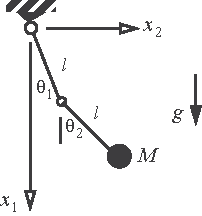
\includegraphics{Figure_18-7.pdf}
\caption{\label{fig18.7}}
\end{wrapfigure}
\begin{equation}\label{ex18.1a}
\vspace*{-2\baselineskip}
\begin{split}
&x_{1}(t)=l \cos \theta_{1}(t)+l \cos \theta_{2}(t) \\&x_{2}(t)=l \sin \theta_{1}(t)+l \sin \theta_{2}(t)
\end{split}.
\end{equation}

\noindent
The kinetic energy is
\begin{align}\label{ex18.1b}
T=\frac{1}{2} M\left[\left(\dot{x}_{1}\right)^{2}+\left(\dot{x}_{2}\right)^{2}\right]=\frac{1}{2} M l^{2}\left[\left(\dot{\theta}_{1}\right)^{2}+\left(\dot{\theta}_{2}\right)^{2}+2 \dot{\theta}_{1} \dot{\theta}_{2} \cos \left(\theta_{1}-\theta_{2}\right)\right].
\end{align}
The potential energy is
\begin{align}\label{ex18.1c}
V=M g\left(2 l-x_{1}-x_{2}\right)=M g l\left[\left(1-\cos \theta_{1}\right)+\left(1-\cos \theta_{2}\right)\right].
\end{align}
Lagrange's equations (\ref{eq18.79}) for the pendulum are
\begin{align}\label{ex18.1d}
\frac{d}{d t}\left(\frac{\partial L}{\partial \dot{\theta}_{1}}\right)-\frac{\partial L}{\partial \theta_{1}}=0 \quad \frac{d}{d t}\left(\frac{\partial L}{\partial \dot{\theta}_{2}}\right)-\frac{\partial L}{\partial \theta_{2}}=0.
\end{align}
Derivatives of the Lagranian function (\ref{eq18.77}) with respect to $\theta_{1}$ and $\dot{\theta}_{1}$ follow.
\begin{gather}\label{ex18.1e}
\frac{\partial L}{\partial \theta_{1}}=-M l^{2} \dot{\theta}_{1} \dot{\theta}_{2} \sin \left(\theta_{1}-\theta_{2}\right)-M g l \sin \theta_{1}, \\
\frac{\partial L}{\partial \dot{\theta}_{1}}=M l^{2}\left[\dot{\theta}_{1}+\dot{\theta}_{2} \cos \left(\theta_{1}-\theta_{2}\right)\right],\text{ and }\frac{d}{d t}\left(\frac{\partial L}{\partial \dot{\theta}_{1}}\right)=M l^{2}\left[\ddot{\theta}_{1}+\ddot{\theta}_{2} \cos \left(\theta_{1}-\theta_{2}\right)-\dot{\theta}_{2}\left(\dot{\theta}_{1}-\dot{\theta}_{2}\right) \sin \left(\theta_{1}-\theta_{2}\right)\right]. \label{ex18.1f}
\end{gather}
Substitute eqs. (\textbf{e}) and (\textbf{f}) into the Lagrangian equation for $\theta_{1}$ in eq. (\textbf{d}) to get the equation of motion
\begin{align}\label{ex18.1g}
M l^{2}\left[\ddot{\theta}_{1}+\ddot{\theta}_{2} \cos \left(\theta_{1}-\theta_{2}\right)+\left(\dot{\theta}_{2}\right)^{2} \sin \left(\theta_{1}-\theta_{2}\right)\right]+M g l \sin \theta_{1}=0.
\end{align}
Similar mathematical manipulations for Lagrange's equation in coordinate $\theta_{2}$ lead to the second equation of motion
\begin{align}\label{ex18.1h}
M l^{2}\left[\ddot{\theta}_{2}+\ddot{\theta}_{1} \cos \left(\theta_{1}-\theta_{2}\right)-\left(\dot{\theta}_{1}\right)^{2} \sin \left(\theta_{1}-\theta_{2}\right)\right]+M g l \sin \theta_{2}=0.\\[-2.6pc] \nonumber
\end{align}
%\hfill\qed
\end{example}

\vspace*{-1.4pc}

\setcounter{equation}{79}
\section{The dynamic response of an elastic thin-walled bar}\label{sec18.6}

Starting with Hamilton's principle we develop a weak form for the dynamic response of a thin-walled bar suitable for a finite element analysis. Assume the bar is homogenous with a uniform cross section along the $z$-axis, $0 \leq z \leq L$, where \textit{L} denotes the length of the bar. Since the bar is a one-dimensional continuum, Hamilton's principle (\ref{eq18.69}) is expressed as
\begin{align}\label{eq18.80}
\int_{t_{0}}^{t_{1}}\left[\int_{0}^{L}(\delta \bar{T}+\delta \bar{W}) d z\right] d t=0,
\end{align}
where $\delta \bar{T}$ is the virtual kinetic energy per unit axial length, and $\delta \bar{W}$ is the virtual work of the non-inertial forces per unit axial length. From eqs. (\ref{eq3.20}) and (\ref{eq3.22}) on page \pageref{eq3.20}, and eq.~(\ref{eq3.26}) on page \pageref{eq3.26}, the displacements of a material point on the contour of the cross section are
\begin{gather}
\label{eq18.81}
u_{s}(s,~z,~t)=-u(z,~t) \sin \theta(s)+v(z,~t) \cos \theta(s)+r_{n}(s) \phi_{z}(z,~t),
\\
\label{eq18.82}
u_{\zeta}(s,~z,~t)=u(z,~t) \cos \theta(s)+v(z,~t) \sin \theta(s)-r_{t}(s) \phi_{z}(z,~t),\ \text{and}
\\
\label{eq18.83}
u_{z}(s,~z,~t)=w(z,~t)+y(s) \phi_{x}(z,~t)+x(s) \phi_{y}(z,~t).
\end{gather}
The virtual kinetic energy term in Hamilton's principle (\ref{eq18.80}) is written as
\begin{align}\label{eq18.84}
\int_{t_{0}}^{t_{1}}\left(\int_{0}^{L} \delta \bar{T} d z\right) d t=\int_{t_{0}}^{t_{1}}\left[\int_{0}^{L}\left(\int_{c} \delta T t d s\right) d z\right] d t,
\end{align}
where the kinetic energy per unit volume, or the kinetic energy density, is
\begin{align}\label{eq18.85}
T=\frac{1}{2} \rho\left[\left(\dot{u}_{s}\right)^{2}+\left(\dot{u}_{\zeta}\right)^{2}+\left(\dot{u}_{z}\right)^{2}\right],
\end{align}
The mass density is denoted by $\rho$. The dot over the displacement function is a shorthand notation for the partial derivative of the function with respect to time; e.g.,
\begin{align}\label{eq18.86}
\dot{u}_{s}=\frac{\partial u_{s}}{\partial t}.
\end{align}
The virtual kinetic energy density at a fixed time is
\begin{align}\label{eq18.87}
\delta T=\frac{\partial T}{\partial \dot{u}_{s}} \delta \dot{u}_{s}+\frac{\partial T}{\partial \dot{u}_{\zeta}} \delta \dot{u}_{\zeta}+\frac{\partial T}{\partial \dot{u}_{z}} \delta \dot{u}_{z}=\rho\left(\dot{u}_{s} \delta \dot{u}_{s}+\dot{u}_{\zeta} \delta \dot{u}_{\zeta}+\dot{u}_{z} \delta \dot{u}_{z}\right),
\end{align}
where $\delta \dot{u}_{s}$, $\delta \dot{u}_{\zeta},\text{ and }\delta \dot{u}_{z}$ are the infinitesimal virtual velocity components. Interchange the order of the temporal and spatial integrals in eq.~(\ref{eq18.84}) to write the virtual kinetic energy term as
\begin{align}\label{eq18.88}
\int_{t_{0}}^{t_{1}}\left[\int_{0}^{L}\left(\int_{c}\delta T t d s\right) d z\right] d t=\int_{0}^{L}\left[\int_{c}\left(\int_{t_{0}}^{t_{1}} \delta T d t\right) t d s\right] d z.
\end{align}
The interior integral in eq.~(\ref{eq18.88}) with respect to time is integrated by parts as follows:
\begin{equation}\label{eq18.89}
\begin{split}\int_{t_{0}}^{t_{1}} \delta T d t &=\rho \int_{t_{0}}^{t_{1}}\left(\dot{u}_{s} \delta \dot{u}_{s}+\dot{u}_{\zeta} \delta \dot{u}_{\zeta}+\dot{u}_{z} \delta \dot{u}_{z}\right) d t \\&=-\rho \int_{t_{1}}^{t_1}\left(\ddot{u}_{s} \delta u_{s}+\ddot{u}_{\zeta} \delta u_{\zeta}+\ddot{u}_{s} \delta u_{s}\right) d t+\left.\rho\left(\dot{u}_{s} \delta u_{s}+\dot{u}_{\zeta} \delta u_{\zeta}+\dot{u}_{z} \delta u_{z}\right)\right|_{t_{0}} ^{t_{1}}\end{split}.
\end{equation}
By Hamilton's principle the virtual displacements $\left\{\delta u_{s}, \delta u_{\zeta}, \delta u_{z}\right\}$ vanish at times $t_{0}$ and $t_{1}$. Return to eq.~(\ref{eq18.84}) and identify
\begin{align}\label{eq18.90}
\int_{t_{0}}^{t_{1}}\left[\int_{0}^{t}\left(\int_c \delta T t d s\right) d z\right] d t=\int_{t_{0}}^{t_{1}}\left[\int_{0}^{L} \delta \bar{T} d z\right] d t,
\end{align}
where the virtual kinetic energy per unit axial length is
\begin{align}\label{eq18.91}
\delta \bar{T}=\int_{c} \delta T t d s=-\rho \int_{c}\left(\ddot{u}_{s} \delta u_{s}+\ddot{u}_{\zeta} \delta u_{\zeta}+\ddot{u}_{s} \delta u_{s}\right) t d s.
\end{align}
We assume the density of mass $\rho$ is independent of the contour coordinate $s$. The individual terms in the integral for $\delta \bar{T}$ are as follows:
\begin{gather}\label{eq18.92}
\rho \int_{c}\left(\ddot{u}_{s} \delta u_{s}\right) t d s=\rho \int_{c}\left[-\ddot{u} \sin \theta+\ddot{v} \cos \theta+r_{n} \ddot{\phi}_{z}\right]\left[-\delta u \sin \theta+\delta v \cos \theta+r_{n} \delta \phi_{z}\right] t d s,
\\\label{eq18.93}
\rho \int_{c}\left(\ddot{u}_{\zeta} \delta u_{\zeta}\right) t d s=\rho \int_{c}\left[\ddot{u} \cos \theta+\ddot{v} \sin \theta-r_{t} \ddot{\phi}_{z}\right]\left[\delta u \cos \theta+\delta v \sin \theta-r_{t} \delta \phi_{z}\right] t d s,\ \text{and}
\\\label{eq18.94}
\rho \int_{c}\left(\ddot{u}_{z} \delta u_{z}\right) t d s=\rho \int_{c}\left[\ddot{w}+y \ddot{\phi}_{x}+x \ddot{\phi}_{y}\right]\left[\delta w+y \delta \phi_{x}+x \delta \phi_{y}\right] t d s.
\end{gather}
Sum eqs. (\ref{eq18.92}) to (\ref{eq18.94}) and collect terms in the integral multiplying the virtual displacements and virtual rotations. In the process of evaluating and simplifying the result for $\delta \bar{T}$, the following terms are identified or defined:
\begin{itemize}
  \item From eq.~(\ref{eq3.9}) on page \pageref{eq3.9} the relationship between normal and tangential coordinates of the contour and the Cartesian coordinates $\{x(s), y(s)\}$ of the contour is
  \begin{align}\label{eq18.95}
r_{n} \cos \theta-r_{t} \sin \theta=x(s)-x_{s c} \quad r_{n} \sin \theta+r_{t} \cos \theta=y(s)-y_{s c}.
\end{align}
  \item From eqs. (\ref{eq4.2}) and (\ref{eq4.3}) on page \pageref{eq4.3} the geometric properties of the cross section are identified as
\begin{align}\label{eq18.96}
A=\int_{c} t d s \quad \int_{c} x t d s=0 \quad \int_{c} y t d s=0 \quad\left(I_{x x}, I_{y y}, I_{x y}\right)=\int_{c}\left(y^{2}, x^{2}, x y\right) t d s.
\end{align}
  \item Terms associated with the mass are defined by
\begin{gather}\label{eq18.97}
m=\rho \int_{c} t d s=\rho A,
\\
\rho\left(I_{x x}, I_{y y}, I_{x y}\right)=\rho A\left(I_{x x}/A, I_{y y}/A, I_{x y}/A\right)=m\left(r_{x}^{2}, r_{y}^{2}, r_{x y}^{2}\right),\ \text{and}\label{eq18.98}\\
I_{z}=\rho \int_{c}\left(r_{n}^{2}+r_{t}^{2}\right) t d s=\rho A\left[\frac{1}{A} \int_{c}\left(r_{n}^{2}+r_{t}^{2}\right) t d s\right] = m r_{z}^{2}.\label{eq18.99}
\end{gather}
\end{itemize}
The mass per unit length is denoted by $m$, rotary inertial moments due to bending by $\rho(I_{x x}, I_{y y}, I_{x y})$, and the polar moment of inertia about the $z$-axis through the shear center by $I_{z}$. The final result for virtual kinetic energy per unit length in eq.~(\ref{eq18.91}) is
\begin{align}\label{eq18.100}
\delta \bar{T} =&-\left\{m\left(\ddot{u}+y_{s c} \ddot{\phi}_{z}\right) \delta u+m\left(\ddot{v}-x_{s c} \ddot{\phi}_{z}\right) \delta v+m \ddot{w} \delta w+m\left(r_{x}^{2} \ddot{\phi}_{x}+r_{x y}^{2} \ddot{\phi}_{y}\right) \delta \phi_{x}+m\left(r_{x y}^{2} \ddot{\phi}_{x}+r_{y}^{2} \ddot{\phi}_{y}\right) \delta \phi_{y}\right.\nonumber\\ &+\left.m\left(r_{z}^{2} \ddot{\phi}_{z}+y_{s c} \ddot{u}-x_{s c} \ddot{v}\right) \delta \phi_{z}\right\}.
\end{align}

The virtual work per unit axial length is determined from conservative forces and non-conservative forces. It is expressed as
\begin{align}\label{eq18.101}
\delta \bar{W}=-\delta \bar{U}+\delta \bar{W}_{\text {n.c.}},
\end{align}
where $\bar{U}$ is the potential energy of the conservative forces and $\delta \bar{W}_{\text {n.c. }}$ is the virtual work of the non-conservative forces acting at point $z$ in the bar. The potential energy per unit length represents the energy due to elastic deformation of the bar and it is given by
\begin{align}\label{eq18.102}
\bar{U}=\bar{U}_{\varepsilon}+\bar{U}_{\gamma}.
\end{align}
The strain energy due extension and bending is denoted by $\bar{U}_{\varepsilon}$, and the strain energy due to transverse shear and torsion by $\bar{U}_{\gamma}$. From eq.~(\ref{eq5.47}) on page \pageref{eq5.47}
\begin{align}\label{eq18.103}
\bar{U}_{\varepsilon}=\frac{1}{2}\left[E A\left(w^{\prime}\right)^{2}+E I_{x x}\left(\phi_{x}^{\prime}\right)^{2}+E I_{y y}\left(\phi_{y}^{\prime}\right)^{2}+2 E I_{x y}\left(\phi_{x}^{\prime}\right)\left(\phi_{y}^{\prime}\right)\right],
\end{align}
and from eq.~(\ref{eq5.82}) on page \pageref{eq5.82}
\begin{align}\label{eq18.104}
\bar{U}_{\gamma}=\frac{1}{2}\left[s_{x x} \psi_{x}^{2}+2 s_{x y} \psi_{x} \psi_{y}+s_{y y} \psi_{y}^{2}+G J\left(\phi_{z}^{\prime}\right)^{2}\right].
\end{align}
Note that the partial derivatives of the axial displacement and bending rotations are denoted by a prime superscript in eq.~(\ref{eq18.103}). That is,
\begin{align}\label{eq18.105}
w^{\prime}=\frac{\partial w}{\partial z} \quad \phi_{x}^{\prime}=\frac{\partial \phi_{x}}{\partial z} \quad \phi_{y}^{\prime}=\frac{\partial \phi_{y}}{\partial z}.
\end{align}
The transverse shear strains in eq.~(\ref{eq18.104}) are related to the displacements and rotations by
\begin{align}\label{eq18.106}
\psi_{x}=u^{\prime}+\phi_{y} \quad \Psi_{y}=v^{\prime}+\phi_{x}.
\end{align}
Refer to figure~\ref{fig3.6} on page \pageref{fig3.6}. The virtual strains are denoted by $\delta w^{\prime}$, $\delta \phi_{x}^{\prime}$, $\delta \phi_{y}^{\prime}$, $\delta \psi_{x}$, $\delta \Psi_{y},\text{ and }\delta \phi_{z}$, where
\begin{align}\label{eq18.107}
\delta \psi_{x}=\delta u^{\prime}+\delta \phi_{y},\text{ and }\delta \psi_{y}=\delta v^{\prime}+\delta \phi_{x}.
\end{align}
 At a fixed value of the coordinate $z$ the virtual strain energies per unit axial length are
\begin{align}\label{eq18.108}
\delta \bar{U}_{\varepsilon}&=\frac{\partial \bar{U}_{\varepsilon}}{\partial w^{\prime}} \delta w^{\prime}+\frac{\partial \bar{U}_{\varepsilon}}{\partial \phi_{x}^{\prime}} \delta \phi_{x}^{\prime}+\frac{\partial \bar{U}_{\varepsilon}}{\partial \phi_{y}^{\prime}} \delta \phi_{y}^{\prime}=N \delta w^{\prime}+M_{x} \delta \phi_{x}^{\prime}+M_{y} \delta \phi_{y}^{\prime},\ \text{and}
\\\label{eq18.109}
\delta \bar{U}_{\gamma} &=\frac{\partial \bar{U}_{\gamma}}{\partial \psi_{x}} \delta \psi_{x}+\frac{\partial \bar{U}_{\gamma}}{\partial \psi_{y}} \delta \psi_{y}+\frac{\partial \bar{U}_{\gamma}}{\partial \phi_{z}^{\prime}} \delta \phi_{z}^{\prime}=V_{x} \delta \psi_{x}+V_{y} \delta \psi_{y}+M_{z} \delta \phi_{z}^{\prime}.
\end{align}
The generalized forces corresponding to the virtual strains in eqs. (\ref{eq18.108}) and (\ref{eq18.109}) are given by
\begin{align}\label{eq18.110}
N=E A w^{\prime} \quad M_{x}=E I_{x x} \phi_{x}^{\prime}+E I_{x y} \phi_{y}^{\prime} \quad M_{y}=E I_{x y} \phi_{x}^{\prime}+E I_{y y} \phi_{y}^{\prime},\ \text{and}\\
\label{eq18.111}
V_{x}=s_{x x} \psi_{x}+s_{x y} \psi_{y} \quad V_{y}=s_{x y} \psi_{x}+s_{y y} \psi_{y} \quad M_{z}=G J \phi_{z}^{\prime}.
\end{align}
The total virtual strain energy is the sum of eqs. (\ref{eq18.108}) and (\ref{eq18.109}). That is,
\begin{align}\label{eq18.112}
\delta \bar{U}=\delta \bar{U}_{\varepsilon}+\delta \bar{U}_{\gamma}=N \delta w^{\prime}+M_{x} \delta \phi_{x}^{\prime}+M_{y} \delta \phi_{y}^{\prime}+V_{x} \delta \psi_{x}+V_{y} \delta \psi_{y}+M_{z} \delta \phi_{z}^{\prime}.
\end{align}
Substitute eq.~(\ref{eq18.101}) into Hamilton's principle (\ref{eq18.80}) to get
\begin{align}\label{eq18.113}
\int_{t_{0}}^{t_{1}}\left[\int_{0}^{L}(\delta \bar{T}+\delta \bar{W}) d z\right] d t=-\int_{t_0}^{t_1}\left[\int_{0}^{L}\left(-\delta \bar{T}+\delta \bar{U}-\delta \bar{W}_{\mathrm{n}, \mathrm{c}.}^{L}\right) d z\right] d t=0.
\end{align}
Equation (\ref{eq18.113}) is satisfied for $t_{0} \leq t \leq t_{1}$ by
\begin{align}\label{eq18.114}
\left[\int_{0}^{L}\left(-\delta \bar{T}+\delta \bar{U}-\delta \bar{W}_{\mathrm{n}, \mathrm{c}.}\right) d z\right]=0.
\end{align}
Substitute eq.~(\ref{eq18.100}) for $\delta \bar{T}$ and eq.~(\ref{eq18.112}) for $\delta \bar{U}$ into eq.~(\ref{eq18.114}) to get the weak form for the elastodynamics of the thin-walled bar as
\begin{align}\label{eq18.115}
\begin{split}
&\int_{0}^{L}\left\{\left[\left(m\left(\ddot{u}+y_{s c} \ddot{\phi}_{z}\right) \delta u+m\left(\ddot{v}-x_{s c} \ddot{\phi}_{z}\right) \delta v+m \ddot{w} \delta w+m\left(r_{x}^{2} \ddot{\phi}_{x}+r_{x y}^{2} \ddot{\phi}_{y}\right) \delta \phi_{x}+m\left(r_{x y}^{2} \ddot{\phi}_{x}+r_{y}^{2} \ddot{\phi}_{y}\right) \delta \phi_{y}+\right.\right.\right. \\
&\left.\left.\quad m\left(r_{z}^{2} \ddot{\phi}_{z}+y_{s c} \ddot{u}-x_{s c} \ddot{v}\right) \delta \phi_{z}\right]+\left[N \delta w^{\prime}+M_{x} \delta \phi_{x}^{\prime}+M_{y} \delta \phi_{y}^{\prime}+V_{x} \delta \psi_{x}+V_{y} \delta \psi_{y}+M_{z} \delta \phi_{z}^{\prime}\right]\right\} d z=\int_{0}^{L} \delta \bar{W}_{\text {n.c. }} d z\end{split}.
\end{align}

\looseness-1{}The non-conservative virtual work is expressed in terms of the prescribed external loads acting on the bar shown in figure~\ref{fig18.8}. The generalized forces acting on the cross sections at $z=0$ and $z=L$ are denoted by $Q_{i}(t)$, $i=1,2, \ldots, 12$. The prescribed distribution of force intensities (F/L) and distribution of moments intensities\break (F-L/L) are functions of coordinate $z$ and time $t$. Distributions $f_{x}(z,~t)$ and $f_{y}(z,~t)$ are resolved at the shear center, and distribution $f_{z}(z,~t)$ is resolved at the centroid. Distributions of moments $m_{x}(z,~t)$ and $m_{y}(z,~t)$ are resolved at the centroid, and distribution $m_{z}(z,~t)$ is resolved at the shear center. Also, refer to figure~\ref{fig3.8}(b) on page \pageref{fig3.8}.

{\def\thefigure{18.8}
\processfigure{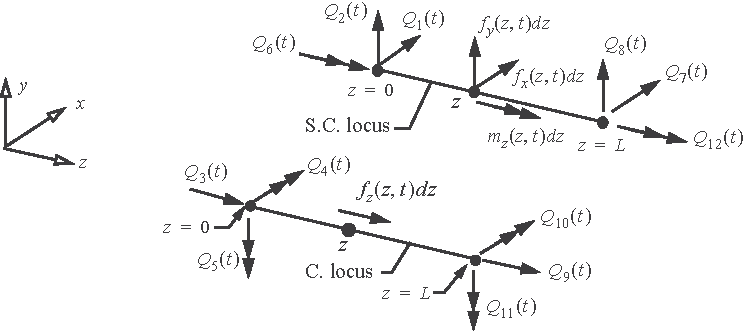
\includegraphics{Figure_18-8.pdf}
}{\caption{External loads acting on the bar.\label{fig18.8}}}}

The virtual displacements and rotations are independent variables. We can take $\delta u$ and its derivative $\delta u'$ not equal to zero, and the remaining virtual displacements and rotations equal to zero in eq.~(\ref{eq18.115}). Then the weak form governing virtual displacement $\delta u$ is
\begin{align}\label{eq18.116}
\int_{0}^{L}\left[\left(m\left(\ddot{u}+y_{s c} \ddot{\phi}_{z}\right) \delta u+V_{x} \delta u^{\prime}\right] d z=\int_{0}^{L} f_{x}(z, t) \delta u(z, t) d z+Q_{1}(t) \delta u(0, t)+Q_{7}(t) \delta u(L, t)\right.\!.
\end{align}
From eq.~(\ref{eq18.115}) and eq.~(\ref{eq18.107}) the weak form governing $\delta v$ and its derivative is
\begin{align}\label{eq18.117}
\int_{0}^{L}\left[m\left(\ddot{v}-x_{s c} \ddot{\phi}_{z}\right) \delta v+V_{y} \delta v^{\prime}\right] d z=\int_{0}^{L} f_{y}(z, t) \delta v(z, t) d z+Q_{2}(t) \delta v(0, t)+Q_{8}(t) \delta v(L, t).
\end{align}
The weak form governing $\delta w$ and its derivative is
\begin{align}\label{eq18.118}
\int_{0}^{L}\left[m \ddot{w} \delta w+N \delta w^{\prime}\right] d z=\int_{0}^{L} f_{z}(z, t) \delta w(z, t) d z+Q_{3}(t) \delta w(0, t)+Q_{9}(t) \delta w(L, t).
\end{align}
The remaining weak forms governing the virtual rotations in the order $\delta \phi_{x}$, $\delta \phi_{y},\text{ and }\delta \phi_{z}$ are as follows:
\begin{align}
&\int_{0}^{L}\left[m\left(r_{x}^{2} \ddot{\phi}_{x}+r_{x y}^{2} \ddot{\phi}_{y}\right) \delta \phi_{x}+M_{x} \delta \phi_{x}^{\prime}+V_{y} \delta \phi_{x}\right] d z\nonumber\\
&\qquad=\int_{0}^{L} m_{x}(z, t) \delta \phi_{x}(z, t) d z+Q_{4}(t) \delta \phi_{x}(0, t)+Q_{10}(t) \delta \phi_{x}(L, t),\label{eq18.119}\\
&\int_{0}^{L}\left[m\left(r_{x y}^{2} \ddot{\phi}_{x}+r_{y}^{2} \ddot{\phi}_{y}\right) \delta \phi_{y}+M_{y} \delta \phi_{y}^{\prime}+V_{x} \delta \phi_{y}\right] d z\nonumber\\*
&\qquad=\int_{0}^{L} m_{y}(z, t) \delta \phi_{y}(z, t) d z+Q_{5}(t) \delta \phi_{y}(0, t)+Q_{11}(t) \delta \phi_{y}(L, t),\ \text{and}\label{eq18.120}\\
&\int_{0}^{L}\left[m\left(r_{z}^{2} \ddot{\phi}_{z}+y_{s c} \ddot{u}-x_{s c} \ddot{v}\right) \delta \phi_{z}+M_{z} \delta \phi_{z}^{\prime}\right] d z\nonumber\\
&\qquad=\int_{0}^{L} m_{z}(z, t) \delta \phi_{z}(z, t) d z+Q_{6}(t) \delta \phi_{z}(0, t)+Q_{12}(t) \delta \phi_{z}(L, t).\label{eq18.121}
\end{align}

\section{Finite element model for the dynamics of an axial bar}\label{sec18.7}

The weak form governing the response of the bar is given by eq.~(\ref{eq18.118}). Following the discussion in article \ref{sec17.2} on page \pageref{sec17.2} consider the mesh
\begin{align}\label{eq18.122}
0=z_{1}<z_{2}<z_{3}<\ldots<z_{M}<z_{M+1}=L,
\end{align}
where \textit{M} denotes the number of elements, and \textit{M+1} is the number of nodes. The $k$th element is denoted by
\begin{align}\label{eq18.123}
\Omega_{k} \equiv\left\{z \mid z_{k} \leq z \leq z_{k+1}\right\} \quad k=1,2, \ldots, M.
\end{align}
Each element is mapped into a standard element denoted by
\begin{align}\label{eq18.124}
\Omega_{\mathrm{st}} \equiv\{\zeta \mid-1<\zeta<1\}.
\end{align}
The standard element is mapped onto the $k$th element by
\begin{align}\label{eq18.125}
z=\eta_{1}(\zeta) z_{k}+\eta_{2}(\zeta) z_{k+1}, \text{where}\ \eta_{1}(\zeta)=(1-\zeta)/2\ \text{and}\ \eta_{2}(\zeta)=(1+\zeta)/2.
\end{align}
The inverse mapping is
\begin{align}\label{eq18.126}
\zeta=\frac{2 z-z_{z}-z_{k+1}}{z_{k+1}-z_{k}}=\frac{2 z-z_{z}-z_{k+1}}{h_{k}} \quad z \in \Omega_{k}.
\end{align}
The length of the element is denoted by $h_{k}$ where $h_{k}=z_{k+1}-z_{k}$. Let $w^{(k)}(z, t)$ denote the axial displacement in $\Omega_k$, which expressed in terms of the nodal displacements and the shape functions is
\begin{align}\label{eq18.127}
w^{(k)}(\zeta, t)=\eta_{1}(\zeta) w_{k}(t)+\eta_{2}(\zeta) w_{k+1}(t) \quad \zeta \in \Omega_{\mathrm{st}}.
\end{align}\begin{align}\label{eq18.128}
\delta w^{(k)}=b_{k} \eta_{1}(\zeta)+b_{k+1} \eta_{2}(\zeta)
\end{align}
The external loads acting on element $\Omega_k$ are shown in figure~\ref{fig18.9}.

Let $\eta_{1}^{\prime}=\frac{d \eta_{1}}{d \zeta}$. The finite element representation of eq.~(\ref{eq18.118}) is
\begin{align}\label{eq18.129}
&\sum_{k=1}^{M} b_{k}\left\{\int_{-1}^1\left[m\left(\eta_{1} \ddot{w}_{k}+\eta_{2} \ddot{w}_{k+1}\right) \eta_{1}+E A \frac{2}{h_{k}}\left(\eta_{1}^{\prime} w_{k}+\eta_{2}^{\prime} w_{k+1}\right) \frac{2}{h_{k}} \eta_{1}^{\prime}\right] \frac{h_{k}}{2} d \zeta\right\} \nonumber\\
&\quad\qquad+ b_{k+1}\left\{\int_{-1}^{1}\left[m\left(\eta_{1} \ddot{w}_{k}+\eta_{2} \ddot{w}_{k+1}\right) \eta_{2}+E A \frac{2}{h_{k}}\left(\eta_{1}^{\prime} w_{k}+\eta_{2}^{\prime} w_{k+1}\right) \frac{2}{h_{k}} \eta_{2}^{\prime}\right] \frac{h_{k}}{2} d \zeta\right\}\nonumber\\
&\qquad=\sum_{k=1}^{M} b_{k}\left[Q_{k}(t)+F_{k}(t)\right]+b_{k+1}\left[Q_{k+1}(t)+F_{k+1}(t)\right] .
\end{align}

\pagebreak

{\def\thefigure{18.9}
\processfigure[!t]{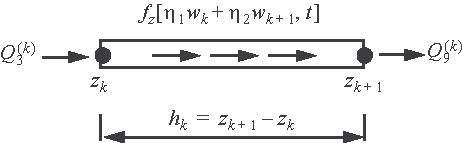
\includegraphics{Figure_18-9.pdf}
}{\caption{External loads acting on axial bar
element $\Omega_k$.\label{fig18.9}}}}

\noindent External loads at a common node between elements are defined by
\begin{align}
Q_{k}(t)=Q_{9}^{(k-1)}(t)+Q_{3}^{(k)}(t) \quad k=2,3, \ldots, M-1,\label{eq18.130}
\end{align}
which are depicted in figure~\ref{fig18.10}.

\vspace*{-12pt}

{\def\thefigure{18.10}
\processfigure[!h]{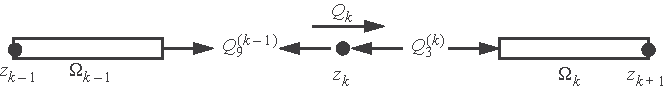
\includegraphics{Figure_18-10.pdf}
}{\caption{\label{fig18.10}}}}

\vspace*{-12pt}

At the first node ${z_1}$ and the last node ${z_{M+1}}$ the external forces are
\begin{align}\label{eq18.131}
Q_{1}(t)=Q_{3}^{(1)}(t),\text{ and }Q_{M}(t)=Q_{9}^{(M)}.
\end{align}
The distributed loads lead to forces
\begin{align}\label{eq18.132}
F_{k}(t)=\int_{-1}^{1} f_{z}\left[\eta_{1} z_{k}+\eta_{2} z_{k+1}, t\right] \eta_{1} \frac{h_{k}}{2} d \zeta \quad F_{k+1}(t)=\int_{-1}^{1} f_{z}\left[\eta_{1} z_{k}+\eta_{2} z_{k+1}, t\right] \eta_{2} \frac{h_{k}}{2} d \zeta.
\end{align}
For $b_{k} \neq 0,\text{ and }b_{k+1}=0$, eq.~(\ref{eq18.129}) leads to
\begin{align}\label{eq18.133}
m h_{k}\left(\frac{1}{3} \ddot{w}_{k}+\frac{1}{6} \ddot{w}_{k+1}\right)+\frac{E A}{h_{k}}\left(w_{k}-w_{k+1}\right)=Q_{k}(t)+F_{k}(t).
\end{align}
For $b_{k}=0$ and $b_{k+1} \neq 0$ eq.~(\ref{eq18.129}) leads to
\[
m h_{k}\left(\frac{1}{6} \ddot{w}_{k}+\frac{1}{3} \ddot{w}_{k+1}\right)+\frac{E A}{h_{k}}\left(-w_{k}+w_{k+1}\right)=Q_{k+1}(t)+F_{k+1}(t).
\]
Finally we write the matrix form for element $\Omega_k$ as
\begin{align}\label{eq18.134}
\frac{m h_{k}}{6}\left[\begin{array}{@{}ll@{}}2 & 1 \\1 & 2\end{array}\right]\left[\begin{array}{@{}c@{}}\ddot{w}_{k} \\\ddot{w}_{k+1}\end{array}\right]+\frac{E A}{h_{k}}\left[\begin{array}{@{}cc@{}}1 & -1 \\-1 & 1\end{array}\right]\left[\begin{array}{@{}c@{}}w_{k} \\w_{k+1}\end{array}\right]=\left[\begin{array}{@{}c@{}}Q_{k}(t)+F_{k}(t) \\Q_{k+1}(t)+F_{k+1}(t)\end{array}\right]
\end{align}
Note that the mass matrix in eq.~(\ref{eq18.134}) is not diagonal, but it is symmetric. This mass matrix is called a \textbf{consistent mass matrix}, since the spatial distribution of the velocity function is consistent with the assumed spatial distribution of the axial displacement function (\ref{eq18.127}).

\begin{example*}[Unrestrained axial motion of a bar]\label{ex18.2}\setcounter{equation}{0}\def\theequation{\alph{equation}}Consider a three-degree-of freedom model of a uniform bar shown in figure~\ref{fig18.11} that undergoes unrestrained axial motion. The mass per unit length $m$ and the axial stiffness $E A$ are constant. The bar is modeled with two finite elements $\Omega_1$ and $\Omega_2$, each with lengths $h_{1}=h_{2}=L$.

{\def\thefigure{18.11}
\processfigure{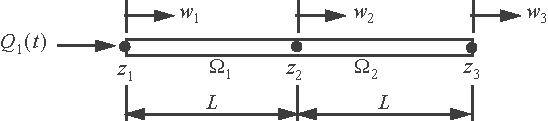
\includegraphics{Figure_18-11.pdf}
}{\caption{Unrestrained axial motion of bar modeled with two elements.\label{fig18.11}}}}

For element $\Omega_1$ the mass and stiffness matrices are
\begin{align}\label{ex18.2a}
M^{(1)}=\frac{m L}{6}
\begin{array}{@{}l@{}}
\hspace*{3pt}{\arraycolsep=2pt\begin{array}{@{}cc@{}}
\ddot{w}_{1} & \ddot{w}_{2}
\end{array}}\\
\left[\begin{array}{@{}ll@{}}2 & 1 \\1 & 2\end{array}\right]
\end{array}
\quad \text{and} \quad K^{(1)}=\frac{E A}{L}
\begin{array}{@{}l@{}}
\hspace*{5pt}{\arraycolsep=6pt\begin{array}{@{}cc@{}}
w_{1} & w_{2}
\end{array}}\\
\left[\begin{array}{@{}cc@{}}1 & -1 \\-1 & 1\end{array}\right]
\end{array}.
\end{align}
For element $\Omega_2$ the mass and stiffness matrices are
\begin{align}\label{ex18.2b}
M^{(2)}=\frac{m L}{6}
\begin{array}{@{}l@{}}
\hspace*{3pt}{\arraycolsep=2pt\begin{array}{@{}cc@{}}
\ddot{w}_{2} & \ddot{w}_{3}
\end{array}}\\
\left[\begin{array}{@{}ll@{}}2 & 1 \\1 & 2\end{array}\right]\end{array} \quad \text{and} \quad K^{(2)}=\frac{E A}{L}
\begin{array}{@{}l@{}}
\hspace*{6pt}{\arraycolsep=5pt\begin{array}{@{}cc@{}}
w_{2} & w_{3}
\end{array}}\\
\left[\begin{array}{@{}cc@{}}1 & -1 \\
-1 & 1\end{array}\right]
\end{array}.
\end{align}
The matrix equation of motion after assembly is
\begin{align}\label{ex18.2c}
\frac{m L}{6}\left[\begin{array}{@{}ccc@{}}2 & 1 & 0 \\1 & 4 & 1 \\0 & 1 & 2\end{array}\right]\left[\begin{array}{@{}c@{}}\ddot{w}_{1} \\\ddot{w}_{2} \\\ddot{w}_{3}\end{array}\right]+\frac{E A}{L}\left[\begin{array}{@{}ccc@{}}1 & -1 & 0 \\-1 & 2 & -1 \\0 & -1 & 1\end{array}\right]\left[\begin{array}{@{}c@{}}w_{1} \\w_{2} \\w_{3}\end{array}\right]=\left[\begin{array}{@{}c@{}}Q_{1}(t) \\0 \\0\end{array}\right].
\end{align}
For the bar at rest at time $t$ = 0 the initial axial displacements are
\begin{align}\label{ex18.2d}
w_{1}(0)=w_{2}(0)=w_{3}(0)=0.
\end{align}
Consider the impulsive response of the bar $Q_{1}(t)=\hat{Q} \delta(t)$, where $\hat{Q}$ is the magnitude of the impulse and $\delta(t)$ is the Dirac delta function. The Dirac delta function is defined by
\begin{align}\label{ex18.2e}
\delta(t)=0\ \text{for}\ t \neq 0,\text{ and }\int_{-\infty}^{\infty} \delta(t) d t=1.
\end{align}

\begin{wrapfigure}[11]{r}{63pt}
\vspace{-19pt}
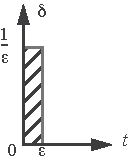
\includegraphics{Figure_18-12.pdf}
\caption{Area under the Dirac delta function.\label{fig18.12}}
\end{wrapfigure}

\vspace*{-1pc}

\noindent The Dirac delta function is depicted in figure~\ref{fig18.12}, in which we take the limit as $\varepsilon \rightarrow 0$. The amplitude of $\delta(0)$ is undefined, but the area under the function is well defined. Note the dimensional units of the Dirac delta function are reciprocal seconds, and the dimensional units of impulse $\hat{Q}$ are force-seconds. The impulsive force causes an initial velocity of the bar. To determine the initial velocity of the bar we integrate the equations of motion (\textbf{c}) with respect to time over an infinitesimal interval at $t$ = 0 from $t=-0$ to $t=+0$. During this time interval there is no displacement of the bar and the velocities $\dot{w}_{i}(-0)=0$, $i=1,2,3$. Integration of eq. (\textbf{c}) over the infinitesimal time interval is
\begin{align}\label{ex18.2f}
\frac{m L}{6}\left[\begin{array}{lll}2 & 1 & 0 \\1 & 4 & 1 \\0 & 1 & 2\end{array}\right]\left[\begin{array}{@{}c@{}}\dot{w}_{1}(+0) \\\dot{w}_{2}(+0) \\\dot{w}_{2}(+0)\end{array}\right]=\hat{Q} \int_{-0}^{+0}\left[\begin{array}{@{}c@{}}\delta(t) \\0 \\0\end{array}\right] d t=\hat{Q}\left[\begin{array}{@{}l@{}}1 \\0 \\0\end{array}\right].
\end{align}
Solve eq. (\textbf{f}) for the initial velocities to get
\begin{align}\label{ex18.2g}
\left[\begin{array}{@{}c@{}}\dot{w}_{1}(+0) \\\dot{w}_{2}(+0) \\\dot{w}_{2}(+0)\end{array}\right]=\frac{\hat{Q}}{m L}\left[\begin{array}{@{}c@{}}7/2 \\-1 \\1/2\end{array}\right].
\end{align}

\subsubsection{Free vibration solution.} Assume a solution $\{w(t)\}=\{\phi\} \cos (\omega t-\alpha)$ to eq. (\textbf{c}), which leads to the generalized eigenvalue problem
\begin{align}\label{ex18.2h}
\left[\begin{array}{@{}ccc@{}}1 & -1 & 0 \\-1 & 2 & -1 \\0 & -1 & 1\end{array}\right]\left[\begin{array}{@{}l@{}}\phi_{1} \\\phi_{2} \\\phi_{3}\end{array}\right]=\lambda\left[\begin{array}{lll}2 & 1 & 0 \\1 & 4 & 1 \\0 & 1 & 2\end{array}\right]\left[\begin{array}{@{}l@{}}\phi_{1} \\\phi_{2} \\\phi_{3}\end{array}\right],
\end{align}
where $\lambda \equiv\left(\frac{m L^{2}}{6 E A}\right) \omega^{2}$. The eigenvalues and modal matrix are
\begin{align}\label{ex18.2i}
\left(\lambda_{1},\left\{\phi_{1}\right\}\right)=\left(2,\left[\begin{array}{@{}c@{}}1 \\-1 \\1\end{array}\right]\right), \left(\lambda_{2},\left\{\phi_{2}\right\}\right)=\left(\frac{1}{2},\left[\begin{array}{@{}c@{}}-1 \\0 \\1\end{array}\right]\right).\ \text{and} \left(\lambda_{3},\left\{\phi_{3}\right\}\right)=\left(0,\left[\begin{array}{@{}l@{}}1 \\1 \\1\end{array}\right]\right).
\end{align}
The eigenvalue $\lambda_{3}=0$ and its associate mode $\{\phi_{3}\}=[\begin{array}{@{}lll@{}}1 & 1 & 1\end{array}]^{T}$ correspond to a rigid body motion of the bar. The non-zero eigenvalues $\lambda_{1}$ and $\lambda_{2}$, and their associated modes correspond to elastic modes of the bar. The frequencies are
\begin{align}\label{ex18.2j}
\omega_{1}=\frac{2 \sqrt{3}}{L} \sqrt{\frac{E A}{m}} \quad \omega_{2}=\frac{\sqrt{3}}{L} \sqrt{\frac{E A}{m}} \quad \omega_{3}=0.
\end{align}

\subsubsection{Transient response.} The transformation from physical displacements to modal displacements is given by
\begin{align}\label{ex18.2k}
\left[\begin{array}{@{}l@{}}w_{1}(t) \\w_{2}(t) \\w_{3}(t)\end{array}\right]=\left[\begin{array}{@{}ccc@{}}1 & -1 & 1 \\-1 & 0 & 1 \\1 & 1 & 1\end{array}\right]\left[\begin{array}{@{}l@{}}q_{1}(t) \\q_{2}(t) \\q_{3}(t)\end{array}\right].
\end{align}
Substitute the transformation (\textbf{k}) into the equations of motion (\textbf{c}) to get equations of motion in modal coordinates:
\begin{align}\label{ex18.2l}
\left[\begin{array}{@{}ccc@{}}\frac{2 L m}{3} & 0 & 0 \\[3pt] 0 & \frac{2 L m}{3} & 0 \\[3pt] 0 & 0 & 2 L m\end{array}\right]\left[\begin{array}{@{}l@{}}\ddot{q}_{1} \\\ddot{q}_{2} \\\ddot{q}_{3}\end{array}\right]+\left[\begin{array}{@{}ccc@{}}\frac{8 E A}{L} & 0 & 0 \\[3pt] 0 & \frac{2 E A}{L} & 0 \\[3pt] 0 & 0 & 0\end{array}\right]\left[\begin{array}{@{}l@{}}q_{1} \\q_{2} \\q_{3}\end{array}\right]=\left[\begin{array}{@{}l@{}}0 \\0 \\0\end{array}\right],\ t>+0.
\end{align}
The initial conditions in modal coordinates are (refer to eq.~(\ref{eq18.27}))
\begin{align}\label{ex18.2m}
\left[\begin{array}{@{}l@{}}q_{1}(0) \\q_{2}(0) \\q_{3}(0)\end{array}\right]=\left[\begin{array}{@{}l@{}}0 \\0 \\0\end{array}\right],\text{ and }\left[\begin{array}{@{}l@{}}\dot{q}_{1}(0) \\\dot{q}_{2}(0) \\\dot{q}_{3}(0)\end{array}\right]=\left[\begin{array}{@{}ccc@{}}\frac{2 L m}{3} & 0 & 0 \\[3pt] 0 & \frac{2 L m}{3} & 0 \\[3pt] 0 & 0 & 2 L m\end{array}\right]^{-1}\left[\begin{array}{@{}ccc@{}}1 & -1 & 1 \\-1 & 0 & 1 \\1 & 1 & 1\end{array}\right]^{T} \frac{m L}{6}\left[\begin{array}{lll}2 & 1 & 0 \\1 & 4 & 1 \\0 & 1 & 2\end{array}\right] \frac{\hat{Q}}{m L}\left[\begin{array}{@{}c@{}}7/2 \\-1 \\1/2\end{array}\right]=\frac{\hat{Q}}{2 m L}\left[\begin{array}{@{}c@{}}3 \\-3 \\1\end{array}\right].
\end{align}
The solution of eq. (\textbf{l}) for the modal displacements are
\begin{align}\label{ex18.2n}
\left[\begin{array}{@{}l@{}}q_{1}(t) \\q_{2}(t) \\q_{3}(t)\end{array}\right]=\frac{\hat{Q}}{2 L m}\left[\begin{array}{@{}c@{}}\frac{3}{\omega_{1}} \sin \omega_{1} t \\[3pt] \frac{-3}{\omega_{2}} \sin \omega_{2} t \\[3pt] t\end{array}\right].
\end{align}
Substitute the modal displacements (\textbf{n}) into eq. (\textbf{k}) to find the results for the response of the physical displacements:
\begin{align}\label{ex18.2o}
\left[\begin{array}{@{}l@{}}w_{1}(t) \\w_{2}(t) \\w_{3}(t)\end{array}\right]=\frac{\hat{Q}}{2 L m}\left[\begin{array}{@{}c@{}}t+\left(3/\omega_{1}\right) \sin \omega_{1} t+\left(3/\omega_{2}\right) \sin \omega_{2} t \\t-\left(3/\omega_{1}\right) \sin \omega_{1} t \\t+\left(3/\omega_{1}\right) \sin \omega_{1} t-\left(3/\omega_{2}\right) \sin \omega_{2} t\end{array}\right].
\end{align}
We specify the following data for an aluminum alloy bar: $L=16\,\text{in.}$, $A=0.2651\,\text{in.}^{2}$, $I_{x x}=0.2985\,\text{in.}^{4}, \text{and } E=9.9 \times 10^{6}\,\text{lb./in.}^{2}$. The mass density $\rho=0.0978\,\mathrm{lbm}/ \mathrm{in.}^{3}$ Convert the pound-mass (lbm) to pound-force (lb.) in the U.S. customary units by recognizing that one pound-force accelerates one pound-mass at the local acceleration of gravity $g$. Thus, $\rho=(0.0978\,\mathrm{lbm}/ \mathrm{in.}^{3})\left(\frac{\mathrm{lb}.}{(1 \mathrm{bm}) 386.4 \mathrm{in}./\mathrm{s}^{2}}\right)=\left(2.531 \times 10^{-4}\right) \frac{\mathrm{lb.-s}^{2}}{\text{in.}^{4}}$, and the mass per unit length is
\begin{align}\label{ex18.2p}
m=\rho A=(2.531 \times 10^{-4}) \frac{1\mathrm{b} \cdot\!\mathrm{-s}^{2}}{\text{in.}^{4}}(0.2651\,\text{in.}^{2})=67.0968 \times 10^{-6} \frac{\mathrm{lb} \cdot\!\mathrm{-s}^{2}}{\text{in.}^{2}}.
\end{align}
The natural frequencies are
\begin{align}\label{ex18.2q}
\omega_{1}=42,819.6\,\mathrm{r}/\mathrm{s}=6,814.94\,\mathrm{Hz} \quad \omega_{2}=21,409.8\,\mathrm{r}/ \mathrm{s}=3,407.47\,\mathrm{Hz} \quad \omega_{3}=0.
\end{align}
Take the impulse $\hat{Q}=6\,\mathrm{lb.-s}$, and compute $\hat{Q}/(2 L m)=2,794.47\,\mathrm{in}./\mathrm{s}$. The transient response for displacements $w_{1}(t)$ and $w_{3}(t)$ for $0 \leq t \leq 2 \tau$ is shown in figure~\ref{fig18.13}. The period for one complete oscillation at the lowest frequency is denoted by $\tau$, where
\begin{align*}
\tau=(2 \pi) /(21,409.8\,\mathrm{s}^{-1})=0.00029347\,\mathrm{s}. \\[-1.45pc]
\text{\hfill\qed\hspace*{-143pt}}
\end{align*}
\end{example*}

\vspace*{-1.5pc}

{\def\thefigure{18.13}
\processfigure{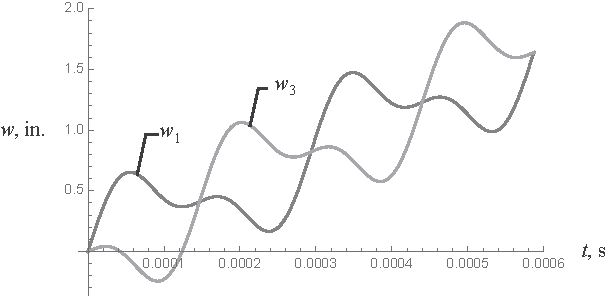
\includegraphics{Figure_18-13.pdf}
}{\caption{Transient
response of the axial
displacements in example \ref{ex18.2}.\label{fig18.13}}}}

%\vspace*{-0.5pc}

\subsection{Truss element}\label{sec18.7.1}

Take one element to represent a truss bar of length \textit{L} at an angle $\theta$ with respect to the \textit{X}-axis connected between the nodes labeled $i$ and $j$ as shown in figure~\ref{fig18.14}(a). Let $h_{k}=L$. The nodal displacements tangent and normal to the bar at node $i$ are denoted by $\left(w_{i}, v_{i}\right)$, respectively, and the nodal displacements tangent and normal to the bar at node $j$ are denoted by $\left(w_{j}, v_{j}\right)$, respectively. The nodal displacements in the \textit{X}- and \textit{Y}- directions to the bar at node $i$ are denoted by $\left(u_{2 i-1}, u_{2 i}\right)$, respectively, and the corresponding nodal displacements at node $j$ are denoted by $\left(u_{2 j-1}, u_{2 j}\right)$, respectively. See figure~\ref{fig18.14}(b).

{\def\thefigure{18.14}
\processfigure{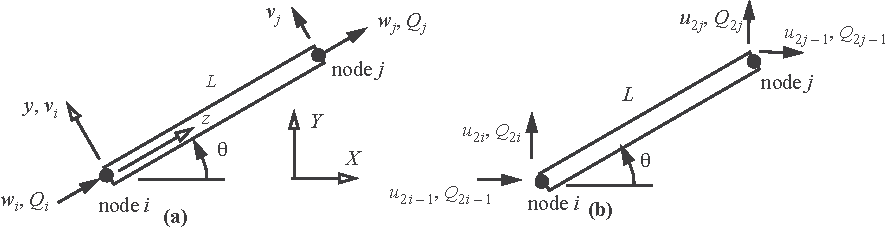
\includegraphics{Figure_18-14.pdf}
}{\caption{(a) Axial bar at an oblique angle. (b) Truss element.\label{fig18.14}}}}


Expand eq.~(\ref{eq18.134}) to include displacements normal to the bar by adding rows and columns of zeros to get\vspace*{0.5pc}
\begin{align}\label{eq18.7a}
\left[\begin{array}{@{}cccc@{}}m L/3 & 0 & m L/6 & 0 \\0 & 0 & 0 & 0 \\m L/6 & 0 & m L/3 & 0 \\0 & 0 & 0 & 0\end{array}\right]\left[\begin{array}{@{}l@{}}\ddot{w}_{i} \\\ddot{v}_{i} \\\ddot{w}_{j} \\\ddot{v}_{j}\end{array}\right]+\left[\begin{array}{@{}cccc@{}}E A/L & 0 & -E A/L & 0 \\0 & 0 & 0 & 0 \\-E A/L & 0 & E A/L & 0 \\0 & 0 & 0 & 0\end{array}\right]\left[\begin{array}{@{}l@{}}w_{i} \\v_{i} \\w_{j} \\v_{j}\end{array}\right]=\left[\begin{array}{@{}c@{}}Q_{i} \\0 \\Q_{j} \\0\end{array}\right].\tag{a}
\end{align}

\pagebreak

\noindent
At node $i$ the displacements in figure~\ref{fig18.14}(a) are related to the displacements in figure~\ref{fig18.14}(b) by $w_{i}=(\cos \theta) u_{2 i-1}+(\sin \theta) u_{2 i},\text{ and }v_{i}=(-\sin \theta) u_{2 i-1}+(\cos \theta) u_{2 i}$. At node $j$ we have similar displacement relations. The nodal displacements are related by matrix
\begin{align}\label{eq18.7b}
\left[\begin{array}{@{}c@{}}w_{i} \\v_{i} \\w_{j} \\v_{j}\end{array}\right]=\left[\begin{array}{@{}cccc@{}}c & s & 0 & 0 \\-s & c & 0 & 0 \\0 & 0 & c & s \\0 & 0 & -s & c\end{array}\right]\left[\begin{array}{@{}c@{}}u_{2 i-1} \\u_{2 i} \\u_{2 j-1} \\u_{2 j}\end{array}\right]=[T(\theta)]\{u\},\tag{b}
\end{align}
where $c=\cos \theta$ and $s=\sin \theta$. Substitute eq. (\textbf{b}) into eq. (\textbf{a}), followed by pre-multiplication by $[T(\theta)]^{T}$ to get
\begin{align}\label{eq18.7c}
[T]^{T}\left[\begin{array}{@{}cccc@{}}m L/3 & 0 & m L/6 & 0 \\0 & 0 & 0 & 0 \\m L/6 & 0 & m L/3 & 0 \\0 & 0 & 0 & 0\end{array}\right][T]\left[\begin{array}{@{}c@{}}\ddot{u}_{2 i-1} \\\ddot{u}_{2 i} \\\ddot{u}_{2 j-1} \\\ddot{u}_{2 j}\end{array}\right]+[T]^{T}\left[\begin{array}{@{}cccc@{}}E A/L & 0 & -E A/L & 0 \\0 & 0 & 0 & 0 \\-E A/L & 0 & E A/L & 0 \\0 & 0 & 0 & 0\end{array}\right][T]\left[\begin{array}{@{}c@{}}u_{2 i-1} \\u_{2 i} \\u_{2 j-1} \\u_{2 j}\end{array}\right]=[T]^{T}\left[\begin{array}{@{}c@{}}Q_{i} \\0 \\Q_{j} \\0\end{array}\right]=\left[\begin{array}{@{}c@{}}Q_{2 i-1} \\Q_{2 i} \\Q_{2 j-1} \\Q_{2 j}\end{array}\right].\tag{c}
\end{align}\setcounter{equation}{134}
The mass matrix for the truss bar is
\begin{align}\label{eq18.135}
[M]=\left[\begin{array}{@{}cccc@{}}c & -s & 0 & 0 \\s & c & 0 & 0 \\0 & 0 & c & -s \\0 & 0 & s & c\end{array}\right]\left[\begin{array}{@{}cccc@{}}m L/3 & 0 & m L/6 & 0 \\0 & 0 & 0 & 0 \\m L/6 & 0 & m L/3 & 0 \\0 & 0 & 0 & 0\end{array}\right]\left[\begin{array}{@{}cccc@{}}c & s & 0 & 0 \\-s & c & 0 & 0 \\0 & 0 & c & s \\0 & 0 & -s & c\end{array}\right]=\frac{m L}{6}\left[\begin{array}{@{}cccc@{}}2 c^{2} & 2 c s & c^{2} & c s \\2 s c & 2 s^{2} & c s & s^{2} \\c^{2} & c s & 2 c^{2} & 2 c s \\c s & s^{2} & 2 s c & 2 s^{2}\end{array}\right].
\end{align}
The stiffness matrix for the truss bar is
\begin{align}\label{eq18.136}
[K]=\left[\begin{array}{@{}cccc@{}}c & -s & 0 & 0 \\s & c & 0 & 0 \\0 & 0 & c & -s \\0 & 0 & s & c\end{array}\right]\left[\begin{array}{@{}cccc@{}}E A/L & 0 & -E A/L & 0 \\0 & 0 & 0 & 0 \\-E A/L & 0 & E A/L & 0 \\0 & 0 & 0 & 0\end{array}\right]\left[\begin{array}{@{}cccc@{}}c & s & 0 & 0 \\-s & c & 0 & 0 \\0 & 0 & c & s \\0 & 0 & -s & c\end{array}\right]=\frac{E A}{L}\left[\begin{array}{@{}cccc@{}}c^{2} & c s & -c^{2} & -c s \\c s & s^{2} & -c s & -s^{2} \\-c^{2} & -c s & c^{2} & c s \\-c s & -s^{2} & c s & s^{2}\end{array}\right].
\end{align}
The stiffness matrix (\ref{eq18.136}) is the same stiffness matrix as determined by the direct stiffness method. See eq.~(\ref{eq16.12}) on page \pageref{eq16.12}.

\pagebreak

\begin{example}[Free vibrations of a three-bar truss]\label{ex18.3}\setcounter{equation}{0}\def\theequation{\alph{equation}}The truss shown in figure~\ref{fig18.15} consists of three bars: 1-2, 1-3, and 1-4. Joints, or nodes, 2, 3, and 4 are fixed and only joint 1 is movable. For all three bars the cross-sectional area $A=475 \times 10^{-6}\,\mathrm{m}^{2}$, the modulus of elasticity $E=70\,\mathrm{GPa}$, and the mass density $\rho=2710\,\mathrm{Kg}/\mathrm{m}^{3}$. The length $L=2\,\mathrm{m}$. Determine the natural frequencies in Hz and the corresponding modal vectors. Normalize the modal vectors such that the component with the largest magnitude is equal to one.

\vspace*{-1\baselineskip}
{\def\thefigure{18.15}
\processfigure{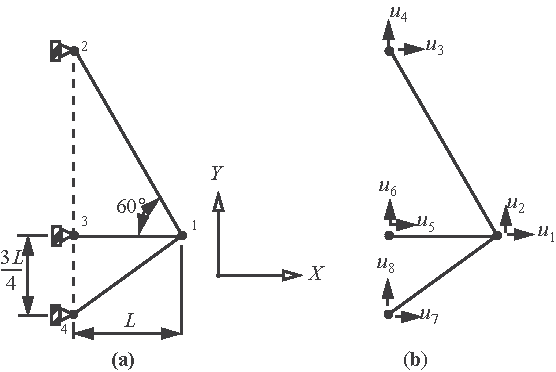
\includegraphics{Figure_18-15.pdf}
}{\caption{Free vibration. (a) Three-bar truss configuration. (b) Nodal displacements.\label{fig18.15}}}}

\subsubsection{Solution.} The unknown nodal displacement vector $\left\{u_{\alpha}(t)\right\}=\left[u_{1}(t) u_{2}(t)\right]^{T}$, and the known nodal displacement vector $\{u_{\beta}(t)\}=[\begin{array}{@{}llllll@{}}u_{3}(t) & u_{4}(t) & u_{5}(t) & u_{6}(t) & u_{7}(t) & u_{8}(t)\end{array}]^{T}=[\begin{array}{@{}llllll@{}}0 & 0 & 0 & 0 & 0 & 0
\end{array}]^{T}$, $t \geq 0$. The length of each bar and the direction cosines are listed in table~\ref{tab18.3}.

\begin{table}[h]%\tab18.3
\processtable{Direction cosines for each truss bar\label{tab18.3}}{%
\begin{tabular}{@{}llllllll@{}}
\toprule
\colhead{Bar} & \colhead{Length} & \colhead{${\boldsymbol\theta}{\bf , deg.}$} & \colhead{c} & \colhead{s}& \colhead{c}$^{\mathbf{2}}$ & \colhead{s}$^{\mathbf{2}}$ & \colhead{cs} \\
\midrule
1-2& $2 L$ & 120& $-1/2$ & $\sqrt{3}/2$ & $1/4$& $3/4$& $-\sqrt{3}/4$ \\
1-3& $L$& 180& $-1$& 0& 1& 0& 0 \\
1-4& $5L/4$& 216.87& $-4/5$& $-3/5$& $16/25$& $9/25$& $12/25$ \\
\botrule
\end{tabular}}{}
\vspace*{-1.5\baselineskip}
\end{table}

From the mass matrix (\ref{eq18.135}) and stiffness matrix (\ref{eq18.136}) for the generic truss bar, we formulate the mass and stiffness matrices for each truss bar in degrees of freedom one and two as follows:
\begin{gather}
\left[K_{1-2}\right]=\frac{E A}{2 L}
\begin{array}[b]{@{}l@{}}
\begin{array}{@{}l}
\hspace*{15pt}1 \hspace*{35pt}2 \hspace*{22pt}3 \hspace*{10pt}4
\end{array}\\
\left[\begin{array}{@{}cccc@{}}1/4 & -\sqrt{3}/4 & \blacksquare & \blacksquare \\
-\sqrt{3}/4 & 3/4 & \blacksquare & \blacksquare \\
\blacksquare & \blacksquare & \blacksquare & \blacksquare\\
\blacksquare & \blacksquare & \blacksquare & \blacksquare
\end{array}\right]\end{array} \quad\left[M_{1-2}\right]=\frac{\rho A(2 L)}{6}
\begin{array}[b]{@{}l@{}}
\begin{array}{@{}l}
\hspace*{15pt}1 \hspace*{35pt}2 \hspace*{22pt}3 \hspace*{10pt}4
\end{array}\\
\left[\begin{array}{@{}cccc@{}}1/2 & -\sqrt{3}/2 & \blacksquare & \blacksquare\\
-\sqrt{3}/2 & 3/2 & \blacksquare& \blacksquare\\
\blacksquare & \blacksquare & \blacksquare & \blacksquare\\
\blacksquare & \blacksquare & \blacksquare & \blacksquare
\end{array}\right]
\end{array}\label{ex18.3a}\\
\left[K_{1-3}\right]=\frac{E A}{L}
\begin{array}[b]{@{}l@{}}
\begin{array}{@{}l}
\hspace*{5pt}1 \hspace*{12pt}2 \hspace*{11pt}5 \hspace*{12pt}6
\end{array}\\
\left[\begin{array}{@{}cccc@{}}
1 & 0 & \blacksquare & \blacksquare \\0 & 0 & \blacksquare & \blacksquare \\\blacksquare & \blacksquare & \blacksquare & \blacksquare\\
\blacksquare & \blacksquare & \blacksquare & \blacksquare\\
\end{array}\right]\end{array} \quad\left[M_{1-3}\right]=\frac{\rho A L}{6}
\begin{array}[b]{@{}l@{}}
\begin{array}{@{}l}
\hspace*{4pt}1 \hspace*{12pt}2 \hspace*{12pt}5 \hspace*{12pt}6
\end{array}\\
\left[\begin{array}{@{}llll@{}}2 & 0 & \blacksquare& \blacksquare \\
0 & 0 & \blacksquare & \blacksquare\\
\blacksquare & \blacksquare & \blacksquare & \blacksquare\\
\blacksquare & \blacksquare & \blacksquare & \blacksquare\end{array}\right]\end{array}\label{ex18.3b}\\
\left[K_{1-4}\right]=\frac{E A}{5 L/4}
\begin{array}[b]{@{}l@{}}
\begin{array}{@{}l}
\hspace*{15pt}1 \hspace*{28pt}2 \hspace*{22pt}7 \hspace*{10pt}8
\end{array}\\
\left[\begin{array}{@{}cccc@{}}
16/25 & 12/25 & \blacksquare & \boldsymbol{\blacksquare} \\12/25 & 9/25 & \boldsymbol{\blacksquare} & \boldsymbol{\blacksquare} \\ \boldsymbol{\blacksquare} & \boldsymbol{\blacksquare}& \boldsymbol{\blacksquare}& \boldsymbol{\blacksquare}\\
\boldsymbol{\blacksquare} & \boldsymbol{\blacksquare}& \boldsymbol{\blacksquare}& \boldsymbol{\blacksquare}\end{array}\right]\end{array} \quad\left[M_{1-4}\right]=\frac{\rho A\left(\frac{5 L}{4}\right)}{6}
\begin{array}[b]{@{}l@{}}
\begin{array}{@{}l}
\hspace*{15pt}1 \hspace*{28pt}2 \hspace*{22pt}7 \hspace*{10pt}8
\end{array}\\
\left[\begin{array}{@{}cccc@{}}32/25 & 24/25 & \boldsymbol{\blacksquare} & \boldsymbol{\blacksquare} \\24/25 & 18/25 & \boldsymbol{\blacksquare} & \boldsymbol{\blacksquare} \\
\boldsymbol{\blacksquare} & \boldsymbol{\blacksquare}& \boldsymbol{\blacksquare}& \boldsymbol{\blacksquare}\\
\boldsymbol{\blacksquare} & \boldsymbol{\blacksquare}& \boldsymbol{\blacksquare}& \boldsymbol{\blacksquare}\end{array}\right]\end{array}\label{ex18.3c}
\end{gather}
Assembly of the structural stiffness matrix in DOFs 1 and 2 results in
\begin{align}\label{ex18.3d}
\left[K_{\alpha \alpha}\right]=\frac{E A}{L}\left[\begin{array}{@{}cc@{}}\frac{1}{8}+1+\left(\frac{4}{5}\right)\left(\frac{16}{25}\right) & \frac{-\sqrt{3}}{8}+0+\left(\frac{4}{5}\right)\left(\frac{12}{25}\right) \\\frac{-\sqrt{3}}{8}+0+\left(\frac{4}{5}\right)\left(\frac{12}{25}\right) & \frac{3}{8}+0+\left(\frac{4}{5}\right)\left(\frac{9}{25}\right)\end{array}\right]=\left[\begin{array}{@{}cc@{}}2.72151 \times 10^{7} & 2.78458 \times 10^{6} \\ 2.78458 \times 10^{6} & 1.10224 \times 10^{7}\end{array}\right] \mathrm{N}/\mathrm{m},
\end{align}
in which $E A/L=16.625 \times 10^{6}\,\mathrm{N}/\mathrm{m}$ was used to get the numerical result for $\left[K_{\alpha \alpha}\right]$. Assembly of the structural mass matrix in DOFs 1 and 2 results in
\begin{align}\label{ex18.3e}
\left[M_{\alpha \alpha}\right]=\frac{\rho A L}{6}\left[\begin{array}{@{}cc@{}}
1+2+\left(\frac{5}{4}\right)\left(\frac{32}{25}\right) & -\sqrt{3}+0+\left(\frac{5}{4}\right)\left(\frac{24}{25}\right) \\-\sqrt{3}+0+\left(\frac{5}{4}\right)\left(\frac{24}{25}\right) & 3+0+\left(\frac{5}{4}\right)\left(\frac{18}{25}\right)\end{array}\right]=\left[\begin{array}{@{}cc@{}}1.97378 & -0.22829 \\-0.22829 & 1.67343\end{array}\right] \mathrm{Kg},
\end{align}
in which $\rho A L=2.5745\,\mathrm{Kg}$ was used to get the numerical result for $\left[M_{\alpha \alpha}\right]$. The matrix eigenvalue problem for the natural frequencies and modes is $\left[K_{\alpha \alpha}\right]\{\phi\}-\lambda\left[M_{\alpha \alpha}\right]\{\phi\}=\{0\}$, where the eigenvalue is $\lambda$ and $\lambda=\omega^{2}$. Written in detail for this structure the matrix eigenvalue problem is
\begin{align}\label{ex18.3f}
\left[\begin{array}{@{}cc@{}}2.72151 \times 10^{7} & 2.78458 \times 10^{6} \\2.78458 \times 10^{6} & 1.10224 \times 10^{7}\end{array}\right]\left[\begin{array}{@{}l@{}}\phi_{1} \\\phi_{2}\end{array}\right]-\lambda\left[\begin{array}{@{}cc@{}}1.97378 & -0.22829 \\-0.22829 & 1.67343\end{array}\right]\left[\begin{array}{@{}l@{}}\phi_{1} \\\phi_{2}\end{array}\right]=\left[\begin{array}{@{}l@{}}0 \\0\end{array}\right].
\end{align}
This eigenvalue system in eq. (\textbf{f}) was solved in \textit{Mathematica} using the function $\text{Eigensystem }\left[\left\{K_{\alpha \alpha}, M_{\alpha \alpha}\right\}\right]$, which finds the generalized eigenvalues and eigenvectors. The eigen pairs are
\begin{align}\label{ex18.3g}
\left(\lambda_{1},\left\{\phi_{1}\right\}\right)=\left(5.92732 \times 10^{6},\left[\begin{array}{@{}c@{}}-0.266679 \\1.0\end{array}\right]\right),\text{ and }\left(\lambda_{2},\left\{\phi_{2}\right\}\right)=\left(1.51655 \times 10^{7},\left[\begin{array}{@{}c@{}}1.0 \\0.435137\end{array}\right]\right).
\end{align}
The natural frequencies are\vspace*{-5pt}
\begin{align}\label{ex18.3h}
\omega_{1} &=\sqrt{5.92732 \times 10^{6}}=2,434.61\,\mathrm{rad}/\mathrm{s}=387.48\,\mathrm{Hz},\text{ and }\nonumber\\ \omega_{2} &=\sqrt{1.51655 \times 10^{7}}=3,894.28\,\mathrm{rad}/\mathrm{s}=619.795\,\mathrm{Hz}\\[-2.3pc] \nonumber
\end{align}
%\hfill\qed
\end{example}

\vspace*{-0.2pc}
\vspace*{-1\baselineskip}

\setcounter{equation}{136}
\section{Dynamic bending of a bar with two axes of symmetry}\label{sec18.8}

If the cross section is symmetric with respect to both the $x$- and $y$-axes through the centroid, then $x_{s c}=y_{s c}=0$, $I_{x y}=0$, $r_{x y}=0,\text{ and }s_{x y}=0$. In this case of double symmetry, transverse bending is decoupled from torsion in both the inertia and stiffness terms. That is, the inertia axis and elastic axis coincide. However, the motions of the lateral displacement $v(z, t)$ and the rotation $\phi_{x}(z, t)$ are linked because of the presence of transverse shear deformation $\psi_{y}$. The governing weak forms (\ref{eq18.117}) and (\ref{eq18.119}) are
\begin{align*}
&\int_{0}^{L}\left[m(\ddot{v}) \delta v+s_{y y}\left(v^{\prime}+\phi_{x}\right) \delta v^{\prime}\right] d z=\int_{0}^{L} f_{y}(z, t) \delta v(z) d z+Q_{2}(t) \delta v(0, t)+Q_{8}(t) \delta v(L, t).\\
&\int_{0}^{L}\left[m\left(r_{x}^{2} \ddot{\phi}_{x}\right) \delta \phi_{x}+E I_{x x} \phi_{x}^{\prime} \delta \phi_{x}^{\prime}+s_{y y}\left(v^{\prime}+\phi_{x}\right) \delta \phi_{x}\right] d z\\
&\quad=\int_{0}^{L} m_{x}(z, t) \delta \phi_{x}(z, t) d z+Q_{4}(t) \delta \phi_{x}(0, t)+Q_{10}(t) \delta \phi_{x}(L, t)
\end{align*}
The previous two equations are combined to the matrix form
\begin{align}\label{eq18.137}
\int_{0}^{L}\left\{\left[\delta \phi_{x} \delta v\right]\left[\begin{array}{@{}cc@{}}m r_{x}^{2} & 0 \\0 & m\end{array}\right]\left[\begin{array}{@{}c@{}}\ddot{\phi}_x \\\ddot{v}\end{array}\right]+\delta \phi_{x}^{\prime} E I_{x x} \phi_{x}^{\prime}+\left(\delta v^{\prime}+\delta \phi_{x}\right) s_{y y}\left(v^{\prime}+\phi_{x}\right)\right\} d z=\delta W_{\mathrm{n}. c},
\end{align}
where the virtual work of the non-conservative forces is
\begin{align}\label{eq18.138}
\delta W_{\text {n.c.}}=\int_{0}^{L}\left[\delta \phi_{x}~\delta v\right]\left[\begin{array}{@{}c@{}}m_{z}(z, t) \\f_{y}(z, t)\end{array}\right] d z+\left[\delta \phi_{x}(0, t) \delta v(0, t)\right]\left[\begin{array}{@{}l@{}}Q_{2}(t) \\Q_{4}(t)\end{array}\right]+\left[\begin{array}{@{}l@{}}\delta \phi_{x}(L, t)~\delta v(L, t)\end{array}\right]\left[\begin{array}{@{}c@{}}Q_{8}(t) \\Q_{10}(t)\end{array}\right].
\end{align}

\subsection{Finite element}\label{sec18.8.1}

The development of the generalized displacements in $\Omega_k$ follows the discussion in article \ref{sec17.3.1} on page \pageref{sec17.3.1}. The lateral displacement of the $k$th element is denoted by $v^{(k)}(\zeta, t)$ and the rotation by $\phi_{x}^{(k)}(\zeta, t)$. Define the generalized external displacements in terms of the rotation and displacement at the nodes by
\begin{align}\label{eq18.139}
v^{(k)}(-1, t)=u_{2 k-1}(t) \quad \phi_{x}^{(k)}(-1, t)=u_{2 k}(t) \quad v^{(k)}(1, t)=u_{2 k+1}(t) \quad \phi_{x}^{(k)}(1, t)=u_{2 k+2}(t).
\end{align}
See figure~\ref{fig18.16}. The 7X1 displacement vector of element $\Omega_k$ is denoted by,
{\def\thefigure{18.16}
\processfigure{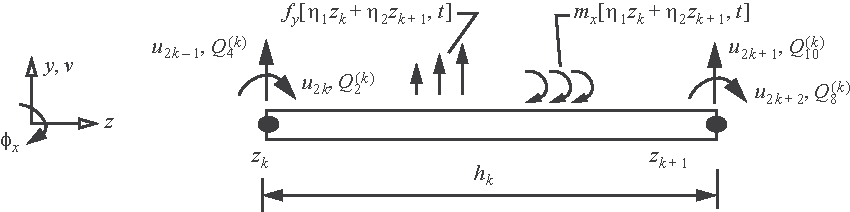
\includegraphics{Figure_18-16.pdf}
}{\caption{Beam element $\Omega_k$.\label{fig18.16}}}}
\begin{align}\label{eq18.140}
\left\{u^{(k)}(t)\right\}=\left[u_{2 k-1}(t)~u_{2 k}(t)~u_{2 k+1}(t)~u_{2 k+2}(t)~u_{1}^{(k)}(t)~u_{2}^{(k)}(t)~u_{3}^{(k)}(t)\right]^{T},
\end{align}
where $u_{1}^{(k)}(t)$, $u_{2}^{(k)}(t),\text{ and }u_{3}^{(k)}(t)$ are internal generalized displacement degrees of freedom. Rotation and displacement functions within the element are expressed in terms of the 2X7 shape function matrix and the 7X1 displacement vector:
\begin{align}\label{eq18.141}
\left[\begin{array}{@{}l@{}}\phi_{x}^{(k)}(\zeta, t) \\v^{(k)}(\zeta, t)\end{array}\right]=[N(\zeta)]\left\{u^{(k)}(t)\right\},
\end{align}
where the shape function matrix is
\begin{align}\label{eq18.142}
[N(\zeta)]=\left[\begin{array}{@{}ccccccc@{}}0 & \eta_{1}(\zeta) & 0 & \eta_{2}(\zeta) & 0 & \eta_{3}(\zeta) & 0 \\\eta_{1}(\eta) & 0 & \eta_{2}(\zeta) & 0 & \eta_{3}(\zeta) & 0 & \eta_{4}(\zeta)\end{array}\right].
\end{align}
The basis functions for the element are
\begin{align}\label{eq18.143}
\eta_{1}(\zeta)=(1-\zeta)/2 \quad \eta_{2}(\zeta)=(1+\zeta)/2 \quad \eta_{3}(\zeta)=\left(\frac{1}{2} \sqrt{\frac{3}{2}}\right)\left(\zeta^{2}-1\right) \quad \eta_{4}(\zeta)=\left(\frac{1}{2} \sqrt{\frac{5}{2}}\right) \zeta\left(\zeta^{2}-1\right).
\end{align}
The virtual rotation and displacement within the element are
\begin{align}\label{eq18.144}
\left[\begin{array}{@{}c@{}}\delta \phi_{x} \\\delta v\end{array}\right]=[N(\zeta)]\left\{b^{(k)}\right\},
\end{align}
where the 7X1 vector $\left\{b^{(k)}\right\}=\left[\begin{array}{@{}lllllll@{}}b_{2 k-1} & b_{2 k} & b_{2 k+1} & b_{2 k+2} & b_{1}^{(k)} & b_{2}^{(k)} & b_{3}^{(k)}\end{array}\right]^{T}$. The virtual generalized displacements $b_{1}^{(k)}$, $b_{2}^{(k)},\text{ and }b_{3}^{(k)}$ correspond to the internal degrees of freedom $u_{1}^{(k)}(t)$, $u_{2}^{(k)}(t),\text{ and }u_{3}^{(k)}(t)$, respectively. The virtual generalized displacement vector $\left\{b^{(k)}\right\}$ is independent of the physical generalized displacement vector $\left\{u^{(k)}\right\}$. The external virtual work of the non-conservative forces (\ref{eq18.138}) for the elements is given by
\begin{align}\label{eq18.145}
\delta W_{\text {n.c. }}=\sum_{k=1}^{M} b_{2 k-1} Q_{2}^{(k)}+b_{2 k} Q_{4}^{(k)}+b_{2 k+1} Q_{8}^{(k)}+b_{2 k+2} Q_{10}^{(k)}+\sum_{k=1}^{M}\left\{b^{(k)}\right\} \int_{-1}^{1}[N]^{T}\left[\begin{array}{@{}c@{}}
m_{x}\\
f_y
\end{array}\right] \frac{h_{k}}{2} d \zeta.
\end{align}
At the common node $z_k$ between elements $\Omega_{k-1}$ and $\Omega_k$ there is an equilibrium relation between the externally applied force $Q_{2 k-1}$ and the externally applied moment $Q_{2 k}$ and the internal actions at the end of element $\Omega_{k-1}$ and the beginning of element $\Omega_{k}$. Refer figure~\ref{fig18.17}. These relations are
{\def\thefigure{18.17}
\processfigure{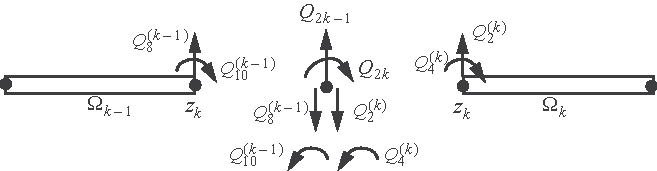
\includegraphics{Figure_18-17.pdf}
}{\caption{Free body
diagram at a node
between two elements\label{fig18.17}}}}
\begin{gather}\label{eq18.146}
Q_{2 k-1}=Q_{8}^{(k-1)}+Q_{2}^{(k)} \quad Q_{2 k}=Q_{10}^{(k-1)}+Q_{4}^{(k)} \quad k=2,3, \ldots, M-1,\ \text{and}\\
\label{eq18.147}
Q_{1}=Q_{2}^{(1)} \quad Q_{2}=Q_{4}^{(1)} \quad Q_{2 M+1}=Q_{8}^{(M)} \quad Q_{2 M+2}=Q_{10}^{(M)}.
\end{gather}
We now write the virtual work of the non-conservative generalized forces as
\begin{align}\label{eq18.148}
\delta W_{\text {n.c. }}=\sum_{k=1}^M\left\{b^{(k)}\right\}\left(\left\{Q^{(k)}\right\}+\left\{F^{(k)}\right\}\right),
\end{align}
where
\begin{align}\label{eq18.149}
\left\{Q^{(k)}\right\}=&\left[Q_{2 k-1} \quad Q_{2 k} \quad Q_{2 k+1} \quad Q_{2 k+2}\quad 0 \quad 0 \quad 0\right]^{T},\text{ and }\nonumber\\
&\left\{F^{(k)}(t)\right\}=\int_{-1}^{1}[N]^{T}\left[\begin{array}{@{}l@{}}m_{x}\left[\eta_{1}(\zeta) z_{k}+\eta_{2}(\zeta) z_{k+1}, t\right] \\f_{y}\left[\eta_{1}(\zeta) z_{k}+\eta_{2}(\zeta) z_{k+1}, t\right]\end{array}\right] \frac{h_{k}}{2} d \zeta.
\end{align}

The partial derivatives with respect to coordinate $z$ in eq.~(\ref{eq18.137}) are replaced by derivatives with respect to dimensionless coordinate $\zeta$ using the chain rule. That is,
\begin{align}\label{eq18.150}
\frac{\partial \phi_{x}}{\partial z}=\frac{\partial \phi_{x}}{\partial \zeta} \frac{d \zeta}{d z}=\frac{2}{h_{k}} \frac{\partial \phi_{x}}{\partial \zeta}=\frac{2}{h_{k}} \phi_{x}^{\prime} \quad d z=\frac{d z}{d \zeta} d \zeta=\frac{h_{k}}{2} d \zeta.
\end{align}
Note that in the following finite element development the prime superscript denotes a derivative with respect to $\zeta$. The derivative of the rotation for element $\Omega_k$ and the virtual rotation are
\begin{align}\label{eq18.151}
\phi_{x}^{\prime}=\left[N_{\phi}(\zeta)\right]\left\{u^{(k)}\right\} \quad \delta \phi_{x}^{\prime}=\left[N_{\phi}(\zeta)\right]\left\{b^{(k)}\right\},
\end{align}
where the 1X7 matrix is given by
\begin{align}\label{eq18.152}
\left[N_{\phi}(\zeta)\right]=\left[\begin{array}{@{}lllllll@{}}0 & \eta_{1}^{\prime} & 0 & \eta_{2}^{\prime} & 0 & \eta_{3}^{\prime} & 0\end{array}\right].
\end{align}
The shear strain for element $\Omega_k$ and the virtual shear strain are
\begin{align}\label{eq18.153}
\left(\frac{2}{h_{k}} v^{\prime}+\phi_{x}\right)=\left[N_{\psi}(\zeta)\right]\left\{u^{(k)}\right\} \quad\left(\frac{2}{h_{k}} \delta v^{\prime}+\delta \phi_{x}\right)=\left[N_{\psi}(\zeta)\right]\{b\},
\end{align}
where the 1X7 matrix is given by
\begin{align}\label{eq18.154}
\left[N_{\psi}(\zeta)\right]=\left[
\begin{array}{@{}lllllll@{}}
\displaystyle\frac{2}{h_{k}} \eta_{1}^{\prime} & \eta_{1} & \displaystyle\frac{2}{h_{k}} \eta_{2}^{\prime} & \eta_{2} & \displaystyle\frac{2}{h_{k}} \eta_{3}^{\prime} & \eta_{3} & \displaystyle\frac{2}{h_{k}} \eta_{4}^{\prime}\end{array}\right].
\end{align}
Substitute eqs. (\ref{eq18.151}) and (\ref{eq18.153}) into the finite element representation of eq.~(\ref{eq18.137}), and substitute eq.~(\ref{eq18.148}) for the virtual work, to get
\begin{align}
&\sum_{k=1}^{M}\left(\{b^{(k)}\}^{T} \int_{-1}^{1}\left([N]^{T}\left[\begin{array}{@{}cc@{}}m r_{x}^{2} & 0 \\0 & m\end{array}\right][N]\{\ddot{u}^{(k)}\}+\frac{2}{h_{k}}[N_{\phi}]^{T} E I_{x x} \frac{2}{h_{k}}[N_{\phi}]\{u^{(k)}\}\right.\right.\nonumber\\
&\qquad\left.\left.+\frac{2}{h_{k}}[N_{\psi}]^{T} s_{y y}[N_{\psi}]\{u^{(k)}\}\right) \frac{h_{k}}{2} d \zeta\right)
=\sum_{k=1}^M\{b^{(k)}\}^{T}(\{Q^{(k)}\}+\{F^{(k)}\}). \label{eq18.155}
\end{align}
We satisfy eq.~(\ref{eq18.155}) for each element in the mesh by
\begin{align}\label{eq18.156}
\left\{b^{(k)}\right\}^{T}\left([M]\left\{\ddot{u}^{(k)}\right\}+[K]\left\{u^{(k)}\right\}-\left(\left\{Q^{(k)}\right\}+\left\{F^{(k)}\right\}\right)\right)=0 \quad \forall\left(\left\{b^{(k)}\right\} \neq 0_{7 X 1}\right).
\end{align}
Hence, the equation of motion for element $\Omega_k$ is
\begin{align}\label{eq18.157}
[M]\left\{\ddot{u}^{(k)}\right\}+[K]\left\{\ddot{u}^{(k)}\right\}=\left\{Q^{(k)}\right\}+\left\{F^{(k)}\right\}.
\end{align}
The mass, and stiffness matrices are
\begin{align}\label{eq18.158}
[M]=\int_{-1}^{1}[N]^{T}\left[\begin{array}{@{}cc@{}}m r_{x}^{2} & 0 \\0 & m\end{array}\right][N] \frac{h_{k}}{2} d \zeta,\text{ and }[K]=\int_{-1}^{1}\left(\frac{2}{h_{k}}\left[N_{\phi}\right]^{T} E I_{x x} \frac{2}{h_{k}}\left[N_{\phi}\right]+\frac{2}{h_{k}}\left[N_{\psi}\right]^{T} s_{y y}\left[N_{\psi}\right]\right) \frac{h_{k}}{2} d \zeta.
\end{align}
Perform the matrix algebra in eq.~(\ref{eq18.158}) to find the 7X7 mass matrix\vspace*{-0.6pc}
\begin{align}\label{eq18.159}
[M]=m h_{k}\left[\begin{array}{@{}ccccccc@{}}
1/3 & 0 & 1/6 & 0 & -1/2 \sqrt{6} & 0 & 1/6 \sqrt{10} \\[3pt]
0 & r_{x}^{2}/3 & 0 & r_{x}^{2}/6 & 0 & -r_{x}^{2}/2 \sqrt{\sqrt{6}} & 0 \\[3pt]
1/6 & 0 & 1/3 & 0 & -1/2 \sqrt{6} & 0 & -1/6 \sqrt{10} \\[3pt]
0 & r_{x}^{2}/6 & 0 & r_{x}^{2}/3 & 0 & -r_{x}^{2}/2 \sqrt{6} & 0 \\[3pt]
-1/2 \sqrt{6} & 0 & -1/2 \sqrt{6} & 0 & 1/5 & 0 & 0 \\[3pt]
0 & -r_{x}^{2} /(2 \sqrt{6}) & 0 & -r_{x}^{2}/2 \sqrt{6} & 0 & r_{x}^{2}/5 & 0 \\[3pt]
1 /(6 \sqrt{10}) & 0 & -1/6 \sqrt{10} & 0 & 0 & 0 & 1/21\end{array}\right].
\end{align}
Perform the matrix algebra in of eq.~(\ref{eq18.158}) to find the 7X7 stiffness matrix\vspace*{-0.6pc}
\begin{align}\label{eq18.160}
[K]=\left[\arraycolsep=2pt\begin{array}{@{}cccccccc@{}}s_{y y}/h_{k} & -s_{y y}/2 & -s_{y y}/h_{k} & -s_{y y}/2 & 0 & s_{y y}/\sqrt{6} & 0 \\[4pt]-s_{y y}/2 & E I_{x x}/h_{k}+h_{k} s_{y y}/3 & s_{y y}/2 & -E I_{x x}/h_{k}+h_{k} s_{y y}/6 & -s_{y y}/ \sqrt{6} & -h_{k} s_{y y}/2 \sqrt{6} & 0 \\[4pt]-s_{y y}/h_{k} & s_{y y}/2 & s_{y y}/h_{k} & s_{y y}/2 & 0 & -s_{y y}/\sqrt{6} & 0 \\[4pt]-s_{y y}/2 & -E I_{x x}/h_{k}+h_{k} s_{y y}/6 & s_{y y}/2 & E I_{x x}/h_{k}+h_{k} s_{y y}/3 & s_{y y}/\sqrt{6} & -h_{k} s_{y y}/2 \sqrt{6} & 0 \\[4pt]
0 & -s_{y y}/\sqrt{6} & 0 & s_{y y}/\sqrt{6} & 2 s_{y y}/h_{k} & 0 & 0 \\[4pt] s_{y y}/\sqrt{6} & -h_{k} s_{y y}/2 \sqrt{6} & -s_{y y}/\sqrt{6} & -h_{k} s_{y y}/2 \sqrt{6} & 0 & 2 E I_{x x}/h_{k}+h_{k}s_{y y}/5 & s_{y y}/\sqrt{15} \\[4pt]
0 & 0 & 0 & 0 & 0 & s_{y y}/\sqrt{15} & 2 s_{y y}/h_{k}\end{array}\right].
\end{align}

\vspace*{-1pc}

\subsection{Method of dynamic condensation}\label{sec18.8.2}

To\enlargethispage{0\baselineskip} eliminate the internal degrees of freedom we employ the Guyan reduction method (Craig, p. 413) and (Qu, 2004, p. 52). The Guyan condensation matrix is determined by ignoring the inertia terms in the internal degrees of freedom. Of course, an error is introduced with respect to the full dynamic model of element $\Omega_k$. Refer to the discussions about the error in the latter references. Let\vspace*{-0.2pc}
\begin{align}\label{eq18.161}
\underbrace{\left\{u^{(k)}\right\}}_{7 X 1}=\underbrace{\left[\begin{array}{@{}c@{}}{\left[I_{4 X 4}\right]} \\{\left[G_{a u}\right]}\end{array}\right]}_{7 X 4}\left[\begin{array}{@{}c@{}}u_{2 k-1} \\u_{2 k} \\u_{2 k+1} \\u_{2 k+2}\end{array}\right]=\left[\begin{array}{@{}c@{}}T_{R}\end{array}\right]\left[\begin{array}{@{}c@{}}u_{2 k-1} \\u_{2 k} \\u_{2 k+1} \\u_{2 k+2}\end{array}\right],
\end{align}

\vspace*{-1.2pc}

\noindent where the 3X4 matrix $\left[G_{a u}\right]$ is the Guyan condensation matrix which was developed in the static condensation procedure of article \ref{sec17.3.3} on page \pageref{sec17.3.3}. Matrix $\left[G_{a q}\right]$ in eq.~(\ref{eq17.102}) on page \pageref{eq17.102} is equal to the matrix $\left[G_{a n}\right]$. The explicit form of eq.~(\ref{eq18.161}) is
\begin{align}\label{eq18.162}
\left[\begin{array}{c} {{u}_{2k-1}} \\ {{u}_{2k}} \\ {{u}_{2k+1}} \\ {{u}_{2k+2}} \\ ---\\{u_{1}^{(k)}} \\ u_{2}^{(k)} \\ u_{3}^{(k)} \end{array} \right]=
\left[ \begin{array}{@{}cccc@{}}
1 & 0 & 0 & 0 \\
0 & 1 & 0 & 0 \\
0 & 0 & 1 & 0 \\
0 & 0 & 0 & 1 \\[3pt] \hdashline\\[-8pt]
0 & \frac{{{h}_{k}}}{2\sqrt{6}} & 0 & \frac{-{{h}_{k}}}{2\sqrt{6}} \\[8pt]
\frac{-\sqrt{6}{{h}_{k}}{{s}_{yy}}}{12E{{I}_{xx}}+\,h_{k}^{2}{{s}_{yy}}} & \frac{\sqrt{3/2}h_{k}^{2}{{s}_{yy}}}{12E{{I}_{xx}}+\,h_{k}^{2}{{s}_{yy}}} & \frac{\sqrt{6}{{h}_{k}}{{s}_{yy}}}{12E{{I}_{xx}}+\,h_{k}^{2}{{s}_{yy}}} & \frac{\sqrt{3/2}h_{k}^{2}{{s}_{yy}}}{12E{{I}_{xx}}+\,h_{k}^{2}{{s}_{yy}}} \\[8pt]
\frac{h_{k}^{2}{{s}_{yy}}}{\sqrt{10}\left( 12E{{I}_{xx}}+\,h_{k}^{2}{{s}_{yy}} \right)} & \frac{-h_{k}^{3}{{s}_{yy}}}{2\sqrt{10}\left( 12E{{I}_{xx}}+\,h_{k}^{2}{{s}_{yy}} \right)} & \frac{-h_{k}^{2}{{s}_{yy}}}{\sqrt{10}\left( 12E{{I}_{xx}}+\,h_{k}^{2}{{s}_{yy}} \right)} & \frac{-h_{k}^{3}{{s}_{yy}}}{2\sqrt{10}12E{{I}_{xx}}+\,h_{k}^{2}{{s}_{yy}}} \\
\end{array} \right]
\left[ \begin{array}{c} {{u}_{2k-1}} \\ {{u}_{2k}} \\ {{u}_{2k+1}} \\ {{u}_{2k+2}} \\\end{array} \right].
\end{align}
The coefficients in the virtual generalized displacements (\ref{eq18.144}) are also transformed through matrix $\left[T_{R}\right]$:
\begin{align}\label{eq18.163}
\underbrace{\left\{b^{(k)}\right\}}_{7 X 1}=\underbrace{\left[T_{R}\right]}_{7 X 4}\left[\begin{array}{@{}c@{}}
b_{2 k-1} \\b_{2 k} \\b_{2 k+1} \\b_{2 k+2}\end{array}\right].
\end{align}
Substitute the transformation for the generalized displacement $\left\{u^{(k)}\right\}$ in eq.~(\ref{eq18.161}), and the transformation of the virtual coefficients (\ref{eq18.163}), into the matrix form of Hamilton's principle (\ref{eq18.156}) to get
\begin{align}\label{eq18.164}
\left[\begin{array}{@{}llll@{}}b_{2 k-1} & b_{2 k} & b_{2 k+1} & b_{2 k+2}\end{array}\right]\left(\left[T_{R}\right]^{T}[M]\left[T_{R}\right]\left[\begin{array}{@{}c@{}}\ddot{u}_{2 k-1} \\\ddot{u}_{2 k} \\\ddot{u}_{2 k+1} \\\ddot{u}_{2 k+2}\end{array}\right]+\left[T_{R}\right]^{T}[K]\left[T_{R}\right]\left[\begin{array}{@{}c@{}}u_{2 k-1} \\u_{2 k} \\u_{2 k+1} \\u_{2 k+2}\end{array}\right]-\left[T_{R}\right]^{T}\left\{Q^{(k)}\right\}+\left\{F^{(k)}\right\}\right]=0.
\end{align}
The previous equation is to be satisfied for every choice of $\left[\begin{array}{@{}llll@{}}b_{2 k-1} & b_{2 k} & b_{2 k+1} & b_{2 k+2}\end{array}\right] \neq 0_{1 X 4}$. Consequently, we obtain the reduced form of the equations of motion in the external degrees of freedom for element $\Omega_k$:
\begin{align}\label{eq18.165}
\left[M_{R}\right]\left[\begin{array}{@{}c@{}}\ddot{u}_{2 k-1} \\\ddot{u}_{2 k} \\\ddot{u}_{2 k+1} \\\ddot{u}_{2 k+2}\end{array}\right]+\left[K_{R}\right]\left[\begin{array}{@{}c@{}}u_{2 k-1} \\u_{2 k} \\u_{2 k+1} \\u_{2 k+2}\end{array}\right]=\{R\}.
\end{align}
The 4X4 symmetric mass matrix $\left[M_{R}\right]$, the 4X4 symmetric stiffness matrix $\left[K_{R}\right]$, and the 4X1 generalized force vector, are given by
\begin{align}\label{eq18.166}
\left[M_{R}\right]=\left[T_{R}\right]^{T}[M]\left[T_{R}\right], \left[K_{R}\right]=\left[T_{R}\right]^{T}[K]\left[T_{R}\right],\ \text{and}\ \{R\}=\left[T_{R}\right]^{T}\left\{Q^{(k)}\right\}+\left\{F^{(k)}\right\}.
\end{align}
The explicit form of the mass matrix is
\begin{align}\label{eq18.167}
\left[M_{R}\right]=m h_{k}\left[\begin{array}{@{}cccc@{}}\mu_{11} & -h_{k} \mu_{12} & \mu_{13} & h_{k} \mu_{14} \\-h_{k} \mu_{21} & h_{k}^{2} \mu_{22} & -h_{k} \mu_{23} & -h_{k}^{2} \mu_{24} \\\mu_{31} & -h_{k} \mu_{32} & \mu_{33} & h_{k} \mu_{34} \\h_{k} \mu_{41} & -h_{k}^{2} \mu_{42} & h_{k} \mu_{43} & h_{k}^{2} \mu_{44}\end{array}\right],
\end{align}
where formulas for the dimensionless coefficients $\mu_{i j}$, $i, j=1,2,3,4$ follow:
\begin{align}\label{eq18.168}
\mu_{11}=\mu_{33}=\frac{1680\left(E I_{x x}\right)^{2}+294 E I_{x x} h_{k}^{2} s_{y y}+h_{k}^{2}\left(13 h_{k}^{2}+42 r_{x}^{2}\right) s_{y y}^{2}}{35\left(12 E I_{x x}+h_{k}^{2} s_{y y}\right)^{2}}
\end{align}\begin{align}\label{eq18.169}
\mu_{21}=\mu_{12}=\mu_{43}=\mu_{34}=\frac{1260\left(E I_{x x}\right)^{2}+21 E I_{x x}\left(11 h_{k}^{2}-60 r_{x}^{2}\right) s_{y y}+h_{k}^{2}\left(11 h_{k}^{2}+21 r_{x}^{2}\right) s_{y y}^{2}}{210\left(12 E I_{x x}+h_{k}^{2} s_{y y}\right)^{2}}
\end{align}\begin{align}\label{eq18.170}
\mu_{31}=\mu_{13}=\frac{3\left(560\left(E I_{x x}\right)^{2}+84 E I_{x x} h_{k}^{2} s_{y y}+h_{k}^{2}\left(3 h_{k}^{2}-28 r_{x}^{2}\right) s_{y y}^{2}\right)}{70\left(12 E I_{x x}+h_{k}^{2} s_{y y}\right)^{2}}
\end{align}\begin{align}\label{eq18.171}
\mu_{41}=\mu_{14}=\mu_{32}=\mu_{23}=\frac{2520\left(E I_{x x}\right)^{2}+126 E I_{x x}\left(3 h_{k}^{2}+20 r_{x}^{2}\right) s_{y y}+h_{k}^{2}\left(13 h_{k}^{2}-42 r_{x}^{2}\right) s_{y y}^{2}}{420\left(12 E I_{x x}+h_{k}^{2} s_{y y}\right)^{2}}
\end{align}\begin{align}\label{eq18.172}
\mu_{22}=\mu_{44}=\frac{126\left(E I_{x x}\right)^{2}\left(h_{k}^{2}+40 r_{x}^{2}\right)+21 E I_{x x} h_{k}^{2}\left(h_{k}^{2}+10 r_{x}^{2}\right) s_{y y}+h_{k}^{4}\left(h_{k}^{2}+14 r_{x}^{2}\right) s_{y y}^{2}}{105 h_{k}^{2}\left(12 E I_{x x}+h_{k}^{2} s_{y y}\right)^{2}}
\end{align}\begin{align}\label{eq18.173}
\mu_{42}=\mu_{24}=\frac{504\left(E I_{x x}\right)^{2}\left(h_{k}^{2}-20 r_{x}^{2}\right)+84 E I_{x x} h_{k}^{2}\left(h_{k}^{2}+10 r_{x}^{2}\right) s_{y y}+h_{k}^{4}\left(3 h_{k}^{2}+14 r_{x}^{2}\right) s_{y y}^{2}}{420 h_{k}^{2}\left(12 E I_{x x}+h_{k}^{2} s_{y y}\right)^{2}},
\end{align}
Note that of the sixteen coefficients $\mu_{i j}$ only six are independent. The 4X4 stiffness matrix $\left[K_{R}\right]$ is the same 4X4 stiffness matrix given by eq.~(\ref{eq17.106}) on page \pageref{eq17.106}.

\begin{example}[Free vibration of a cantilever beam]\label{ex18.4}\setcounter{equation}{0}\def\theequation{\alph{equation}}Consider the homogeneous, uniform cantilever beam shown in figure~\ref{fig18.18}(a). The beam is a thin-walled tube with the data from example~\ref{ex6.5} on page \pageref{ex6.5}. The length $l = 0.8$ m, cross-sectional area $A=171.014 \times 10^{-6}\,\mathrm{m}^{2}$, second area moment $I_{x x}=124.25 \times 10^{-9}\,\mathrm{m}^{4}$, radius of gyration $r_{x}=\sqrt{I_{x x}/A}=0.026955\,\mathrm{m}$, modulus of elasticity $E=68.3\,\mathrm{GPa}$, transverse shear coefficient $s_{y y}=2.195\,\mathrm{MN}$, and the mass density $p=2{,}710\,\mathrm{Kg}./\mathrm{m}^{3}$. The flexural stiffness $E I_{x x}=8,486.28\,\mathrm{N}\mbox{-}\mathrm{m}^{2}$.

Determine the natural frequencies in Hz and the corresponding vibration modes for the one-element model shown in figure~\ref{fig18.18}(b).

{\def\thefigure{18.18}
\processfigure{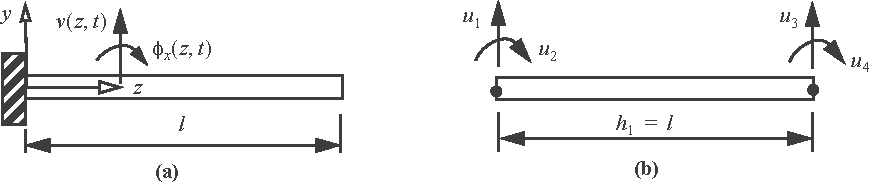
\includegraphics{Figure_18-18.pdf}
}{\caption{(a) Cantilever beam. (b) One-element model.\label{fig18.18}}}}

\subsubsection{Solution.} Generalized displacements $u_{1}(t)=u_{2}(t)=0$ for all $t \geq 0$. So formulate the restrained structural stiffness matrix, and the mass matrix, in DOFs 3 and 4. The total mass of the beam is $m h_{1}=\rho A h_{1}=0.37075\,\mathrm{Kg}$. The numerical result for the 4X4 mass matrix (\ref{eq18.167}) is
\begin{align}\label{ex18.4a}
\left[M_{R}\right]=\frac{m h_{1}}{420}\left[\begin{array}{@{}cccc@{}}\ddot{u}_{1} & \ddot{u}_{2} & \ddot{u}_{3} & \ddot{u}_{4} \\155.29 & -17.3257 & 54.7098 & 10.6725 \\-17.3257 & 2.55726 & -10.6725 & -1.9736 \\\hdashline\\[-8.5pt] 54.7098 & -10.6725 & 155.29 & 17.3275 \\10.6725 & -1.9736 & 17.3275 & 2.55726\end{array}\right]=\left[\begin{array}{@{}l@{}}{\left[M_{\beta \beta}\right]\left[\begin{array}{@{}c@{}}M_{\beta \alpha}\end{array}\right]} \\{\left[M_{\alpha \beta}\right]\left[M_{\alpha \alpha}\right]}\end{array}\right].
\end{align}
The numerical evaluation of the 4X4 stiffness matrix is
\begin{align}\label{ex18.4b}
\left[K_{R}\right]=\left[\begin{array}{@{}cccc@{}}
u_{1} & u_{2} & u_{3} & u_{4} \\
185461 . & -74184.2 & -185461 . & -74184.2 \\
-74184.2 & 40281.8 & 74184.2 & 19065.6 \\
\hdashline\\[-8.5pt]
-185461 & 74184.2 & 185461 . & 74184.2 \\
-74184.2 & 19065.6 & 74184.2 & 40281.8
\end{array}\right]=\left[\begin{array}{@{}c@{}}
{\left[K_{\beta \beta}\right]\left[\begin{array}{@{}c@{}}
K_{\beta \alpha}
\end{array}\right]} \\
\left.\left[K_{\beta \alpha}\right]\left[K_{\alpha \alpha}\right]\right]
\end{array}\right]\!.
\end{align}
The mass and stiffness matrices are partitioned in terms of known and unknown generalized displacements as shown in eqs. (\textbf{a}) and (\textbf{b}). The equations of motion for the generalized displacements $u_{3}(t)$ and $u_{4}(t)$ are
\begin{align}\label{ex18.4c}
\left[M_{\alpha \alpha}\right]\left[\begin{array}{@{}l@{}}\ddot{u}_{3} \\\ddot{u}_{4}\end{array}\right]+\left[K_{\alpha \alpha}\right]\left[\begin{array}{@{}l@{}}u_{3} \\u_{4}\end{array}\right]=\left[\begin{array}{@{}l@{}}0 \\0\end{array}\right].
\end{align}
Assume a harmonic motion given by the equation
\begin{align}\label{ex18.4d}
\left[\begin{array}{@{}l@{}}u_{3}(t) \\u_{4}(t)\end{array}\right]=\left[\begin{array}{@{}l@{}}q_{3} \\q_{4}\end{array}\right] \cos (\omega t-\alpha).
\end{align}
Substitute eq. (\textbf{d}) into the equation of motion (\textbf{c}) to get
\begin{align}\label{ex18.4e}
\left(\left[K_{\alpha \alpha}\right]-\lambda\left[M_{\alpha \alpha}\right]\right)\left[\begin{array}{@{}l@{}}q_{3} \\q_{4}\end{array}\right]=0,\ \text{or}\ \left(\left[\begin{array}{@{}cc@{}}18,5461 & 74,184.2 \\74,184.2 & 40,281.8\end{array}\right]-\lambda\left[\begin{array}{@{}cc@{}}0.137083 & 0.0152959 \\0.0152959 & 0.00225743\end{array}\right]\right)\left[\begin{array}{@{}l@{}}q_{3} \\q_{4}\end{array}\right]=\left[\begin{array}{@{}l@{}}0 \\0\end{array}\right],
\end{align}
where $\lambda=\omega^{2}$. The eigenvalues and eigenvectors are
\begin{align}\label{ex18.4f}
\left(\lambda_{1},\left\{q_{1}\right\}\right)=\left(541,936,\left[\begin{array}{@{}c@{}}-0.509895 \\0.860236\end{array}\right]\right) \quad\left(\lambda_{2},\left\{q_{2}\right\}\right)=\left(4.80887 \times 10^{7},\left[\begin{array}{@{}c@{}}-0.102686 \\0.994714\end{array}\right]\right).
\end{align}
The frequencies in Hertz are
\begin{align}\label{ex18.4g}
\omega_{1}=\sqrt{\lambda_{1}} /(2 \pi)=117.164\,\mathrm{Hz} \quad \omega_{2}=\sqrt{\lambda_{2}} /(2 \pi)=1,103.68\,\mathrm{Hz}.
\end{align}
The lateral displacement for the first vibration mode is given by
\begin{align}\label{ex18.4h}
v_{1}(\zeta)=\eta_{2}(\zeta)\left(q_{3}\right)_{1}+\eta_{3}(\zeta)\left(u_{1}^{(1)}\right)_{1}+\eta_{4}(\zeta)\left(u_{3}^{(1)}\right)_{1},
\end{align}
where the interior generalized displacements for mode one are determined from
\begin{align}\label{ex18.4i}
\left[\begin{array}{@{}l@{}}u_{1}^{(1)} \\[4pt] u_{2}^{(1)} \\[4pt] u_{3}^{(1)}\end{array}\right]_{1}=\left[G_{a u}\right]\left[\begin{array}{@{}l@{}}0 \\0 \\q_{3} \\q_{4}\end{array}\right]_{1}.
\end{align}
The 3X4 matrix $\left[G_{a u}\right]$ is obtained from the last three rows of eq.~(\ref{eq18.162}). Its numerical evaluation is
\begin{align}\label{ex18.4j}
\left[G_{a u}\right]=\left[\begin{array}{@{}cccc@{}}0 & 0.163299 & 0 & -0.163299 \\-2.85495 & 1.14198 & 2.85495 & 1.14198 \\0.294858 & -0.117943 & -0.294858 & -0.117943\end{array}\right].
\end{align}
The interior generalized displacement vector for the first mode is
\begin{align}\label{ex18.4k}
\left[\begin{array}{@{}l@{}}u_{1}^{(1)} \\[4pt] u_{2}^{(1)} \\[4pt] u_{3}^{(1)}\end{array}\right]_{1}=\left[\begin{array}{@{}cccc@{}}0 & 0.163299 & 0 & -0.163299 \\-2.85495 & 1.14198 & 2.85495 & 1.14198 \\0.294858 & -0.117943 & -0.294858 & -0.117943\end{array}\right]\left[\begin{array}{@{}c@{}}0 \\0 \\-0.509895 \\0.860236\end{array}\right]=\left[\begin{array}{@{}l@{}}-0.14047568 \\-0.47335242 \\0.048887805\end{array}\right]\!.
\end{align}
Hence, the expression for the lateral displacement in the first mode is
\begin{align}\label{ex18.4l}
v_{1}(\zeta)=\eta_{2}(\zeta)(-0.509895)+\eta_{3}(\zeta)(-0.14047568)+\eta_{4}(\zeta)(0.048887805).
\end{align}
The lateral displacement for the second vibration mode is given by
\begin{align}\label{ex18.4m}
v_{2}(\zeta)=\eta_{2}(\zeta)\left(q_{3}\right)_{2}+\eta_{3}(\zeta)\left(u_{1}^{(1)}\right)_{2}+\eta_{4}(\zeta)\left(u_{3}^{(1)}\right)_{2}, \end{align}
where the interior generalized displacements for mode two are determined from
\begin{align}\label{ex18.4n}
\left[\begin{array}{@{}c@{}}u_{1}^{(1)} \\[4pt] u_{2}^{(1)} \\[4pt] u_{3}^{(1)}\end{array}\right]_{2}=\left[G_{a u}\right]\left[\begin{array}{@{}c@{}}0 \\0 \\q_{3} \\q_{4}\end{array}\right]_{2}
\end{align}
Numerical evaluation for the interior generalized displacement vector in the second mode is
\begin{align}\label{ex18.4o}
\left[\begin{array}{@{}l@{}}u_{1}^{(1)} \\[4pt] u_{2}^{(1)} \\[4pt] u_{3}^{(1)}\end{array}\right]_{2}=\left[\begin{array}{@{}cccc@{}}0 & 0.163299 & 0 & -0.163299 \\-2.85495 & 1.14198 & 2.85495 & 1.14198 \\0.294858 & -0.117943 & -0.294858 & -0.117943\end{array}\right]\left[\begin{array}{@{}c@{}}0 \\0 \\-0.102686 \\0.994714\end{array}\right]=\left[\begin{array}{@{}c@{}}-0.1624358 \\0.8427801 \\-0.087041765\end{array}\right].
\end{align}
Hence, the lateral displacement in the second mode is
\begin{align}\label{ex18.4p}
v_{2}(\zeta)=\eta_{2}(\zeta)(-0.102686)+\eta_{3}(\zeta)(-0.1624358)+\eta_{4}(\zeta)(-0.087041765).
\end{align}
For this two-degree-of-freedom model there is no prediction of the third and higher frequencies.
\end{example}

For the cantilever beam of example~\ref{ex18.4}, numerical analyses were conducted with two to sixteen equally spaced condensed elements. The details are omitted here, but the results for the first four frequencies are listed in table~\ref{tab18.4}. The frequencies decrease with increasing mesh refinement, and the lowest two frequencies are converging to 116.4\,Hz and 668\,Hz, respectively. The last row in the table lists the frequencies from a continuum analysis of the cantilever beam using Euler-Bernnolli beam theory. The inclusion of transverse shear deformation and rotary inertia in the finite element model result in lower values for the frequencies with respect to the Euler-Bernnolli theory, particularly in the higher frequencies.

The lateral displacement for the first four modes of the cantilever beam are shown in figure~\ref{fig18.19}. The mode shapes were plotted such that the tip displacement was set equal to 0.2 m for clarity in the plots. The lateral displacement passes through zero in the open domain $0<z<0.8\,\mathrm{m}$ once for mode two, twice for mode three, and thrice for mode four. These zeros crossings are called vibration nodes. Vibration nodes are not to be confused with finite element nodes.

\pagebreak

\begin{table}
\processtable{Free vibration frequencies of the cantilever beam\label{tab18.4}}{%
\begin{tabular}{@{}lllll@{}}
\toprule
\colhead{Number of condensed elements} & \colhead{$\omega_{\textbf{1}}$, Hz} & \colhead{$\omega_{\textbf{2}}$, Hz} & \colhead{$\omega_{\textbf{3}}$, Hz}& \colhead{$\omega_{\textbf{4}}$, Hz} \\
\midrule
1& 117.2& 1,103.7& -----& ----- \\
2& 116.5& 682.0& 2,344.4& 6,153.1 \\
4& 116.4& 672.5& 1,735.9& 3,109.9 \\
8& 116.4& 669.2& 1,691.1& 2,979.9 \\
16& 116.4& 668.4& 1,679.2& 2,920.3 \\
\botrule
Euler-Bernoulli$^{\rm a}$ & 118.3& 741.5& 2,076.2& 4,068.8 \\
\end{tabular}}{\footnotesize $^{\rm a}$The free vibration analysis of a continuum model of the cantilever beam using Euler-Bernoulli theory ($\psi_y = 0$ and $s_{yy}\rightarrow \infty$) is from the text by Craig (1981, p. 215).}
\vspace*{-1pc}
\end{table}

{\def\thefigure{18.19}
\processfigure{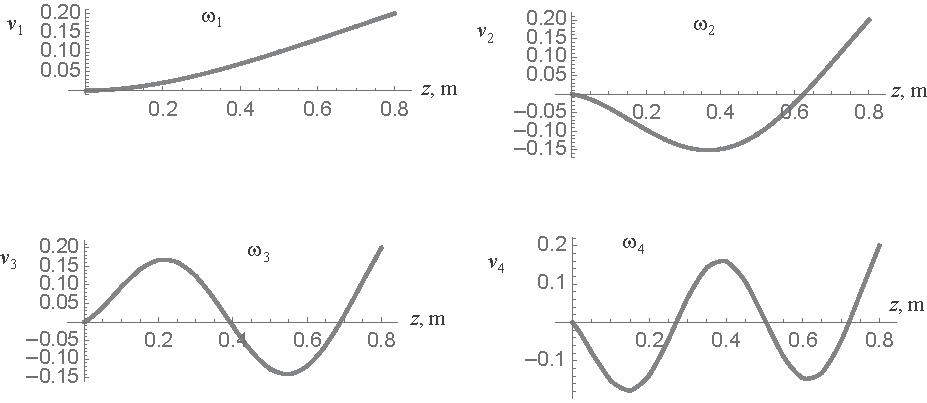
\includegraphics{Figure_18-19.pdf}
}{\caption{First four vibration modes of the cantilever beam.\label{fig18.19}}}}

\vspace*{-0.8pc}

\setcounter{equation}{173}
\section{Vibrations of a coplanar frame}\label{sec18.9}

A bar in a coplanar frame is subject to extension and bending. In the local \textit{x-y-z} coordinates of a bar, we assume that it is symmetric with the respect to the longitudinal \textit{x-z} plane and the \textit{y-z} plane as in article \ref{sec18.8}. The dynamic response of the bar for extension and bending in its \textit{y-z} plane is governed by eq.~(\ref{eq18.115}) on page \pageref{eq18.115}, which reduces~to
\begin{align}\label{eq18.174}
&\int_{0}^{L}\left(m \ddot{v} \delta v+m \ddot{w} \delta w+m r_{x}^{2} \ddot{\phi}_{x} \delta \phi_{x}+N \delta\left(\frac{\partial w}{\partial z}\right)+M_{x} \delta\left(\frac{\partial \phi_{x}}{\partial z}\right)+V_{y} \delta \psi_{y}\right) d z\nonumber\\
&\quad =\left.\left[Q_{2} \delta v+Q_{3} \delta w+Q_{4} \delta \phi_{x}\right]\right|_{z=0}+\left.\left[Q_{8} \delta v+Q_{9} \delta w+Q_{10} \delta \phi_{x}\right]\right|_{z=L}\nonumber\\
&\qquad +\int_{0}^{L} f_{y}(z, t) \delta v(z) d z+\int f_{z}(z, t) \delta w(z) dz.
\end{align}
We use Euler-Bernoulli theory so that transverse shear strain $\Psi_{y}=0$, which means the cross-sectional rotation$.\phi_{x}=-\left(\frac{\partial v}{\partial z}\right)$. Also, neglect the rotary inertia $m r^2_{x}\ddot{\phi}_x$ in eq.~(\ref{eq18.174}). Ignoring rotary inertia and transverse shear deformation has negligible effect on the first few modes of vibration for slender bars (Langhaar, p. 288) . Let one finite element model the bar so that $L=h_{k}$ and $z=\eta_{1}(\zeta) L$. The frame element is shown in its reference configuration in figure~\ref{fig18.20}(a) and in rotated configuration in figure~\ref{fig18.20}(b). The 6X1 displacement vector of the frame element shown in figure~\ref{fig18.20}(a) is
\begin{align}\label{eq18.175}
\{\bar{u}(t)\}=\left[\begin{array}{@{}llllll@{}}w_{3} & v_{2} & \phi_{4} & w_{9} & v_{8} & \phi_{10}\end{array}\right]^{T}.
\end{align}

{\def\thefigure{18.20}
\processfigure{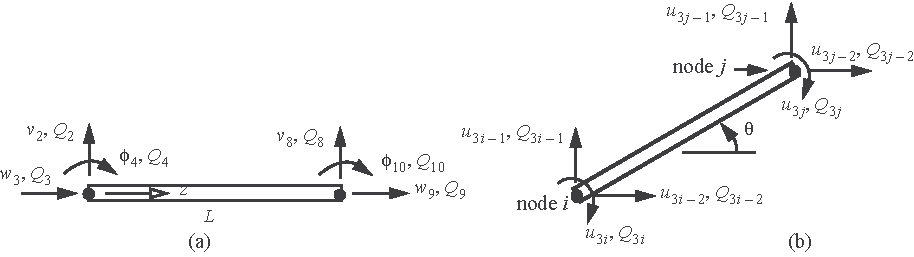
\includegraphics{Figure_18-20.pdf}
}{\caption{(a) Reference frame element. (b) Rotated frame element.\label{fig18.20}}}}

\noindent The displacements are expressed as
\begin{align}\label{eq18.176}
\left[\begin{array}{@{}l@{}}v(\zeta, t) \\w(\zeta, t)\end{array}\right]=[N(\zeta)]\{\bar{u}(t)\},
\end{align}
where the interpolation matrix is
\begin{align}\label{eq18.177}
[N(\zeta)]=\left[\begin{array}{@{}cccccc@{}}0 & \phi_{1}(\zeta) & \phi_{2}(\zeta) & 0 & \phi_{3}(\zeta) & \phi_{4}(\zeta) \\\eta_{1}(\zeta) & 0 & 0 & \eta_{2}(\zeta) & 0 & 0\end{array}\right].
\end{align}
The interpolation functions for the lateral displacement $\phi_{i}(\zeta)$, $i=1,2,3,4$, are the Hermite cubic interpolation functions given by eq.~(\ref{eq17.140}) on page \pageref{eq17.140}. The virtual displacements have the same interpolation as the displacements,
\begin{align}\label{eq18.178}
\left[\begin{array}{@{}l@{}}\delta v(\zeta, t) \\\delta w(\zeta, t)\end{array}\right]=[N(\zeta)]\{b\},
\end{align}
where the 6X1vector $\{b\}$ given in the following equation is independent of the nodal displacements
\begin{align}\label{eq18.179}
\{b\}=\left[\begin{array}{@{}llllll@{}}b_{3} & b_{2} & b_{4} & b_{9} & b_{8} & b_{10}\end{array}\right]^{T}.
\end{align}
The weak form for the element is
\begin{align}\label{eq18.180}
&\int_{-1}^{1}\left([\delta v b w]
\left[\begin{array}{@{}cc@{}}m & 0 \\0 & m
\end{array}\right]
\left[\begin{array}{@{}c@{}}\ddot{v} \\\ddot{v}\end{array}\right]
+\left[\left(\frac{2}{L}\right)^{2} \delta v^{\prime \prime}\left(\frac{2}{L}\right) \delta w^{\prime}\right]
\left[\begin{array}{@{}cc@{}}E I_{x x} & 0 \\0 & E A\end{array}\right]
\left[\begin{array}{@{}l@{}}\left(\frac{2}{L}\right)^{2} v^{\prime \prime} \\[4pt] \left(\frac{2}{L}\right) w^{\prime}\end{array}\right]\right)\left[\frac{L}{2} d \zeta\right.\nonumber\\
&\quad=\{b\}^{T}\{Q\}+\int_{-1}^{1}[\delta v \delta w]\left[\begin{array}{@{}c@{}}f_{y}\left(\eta_{1}(L, t)\right) \\[4pt]
f_{x}\left(\eta_{1}(L, t)\right)\end{array}\right] \frac{L}{2} d \zeta,
\end{align}
where the prime superscript means the derivative with respect to $\zeta$, and the generalized force vector is
\begin{align}\label{eq18.181}
\{Q\}=\left[\begin{array}{@{}llllll@{}}Q_{3} & Q_{2} & Q_{4} & Q_{9} & Q_{8} & Q_{10}\end{array}\right]^{T}.
\end{align}
The displacement derivatives with respect to $\zeta$ appearing in the stiffness terms of eq.~(\ref{eq18.180}) are written in the matrix form
\begin{align}\label{eq18.182}
\left[\begin{array}{@{}c@{}}\left(\frac{2}{L}\right)^{2} v^{\prime \prime} \\\left(\frac{2}{L}\right) w^{\prime}\end{array}\right]=\left[\begin{array}{@{}cc@{}}\left(\frac{2}{L}\right)^{2} \frac{d^{2}}{d \zeta^{2}} & 0 \\0 & \left(\frac{2}{L}\right) \frac{d}{d \zeta}\end{array}\right]\left[\begin{array}{@{}c@{}}v \\w\end{array}\right]=[D N(\zeta)]\{\bar{u}\},
\end{align}
where the 2X6 matrix relating the derivatives of the displacements to the displacement vector is given by
\begin{align}\label{eq18.183}
[D N(\zeta)]=
\left[\begin{array}{@{}cc@{}}\left(\frac{2}{L}\right)^{2} \frac{d^{2}}{d \zeta^{2}} & 0 \\0 & \left(\frac{2}{L}\right) \frac{d}{d \zeta}\end{array}\right][N(\zeta)]=
\left[\begin{array}{@{}cccccc@{}}
0 & \left(\frac{2}{L}\right)^2\phi_{1}^{\prime\prime} & \left(\frac{2}{L}\right)^2\phi_{2}^{\prime\prime} & 0 &
\left(\frac{2}{L}\right)^2\phi_{3}^{\prime\prime} & \left(\frac{2}{L}\right)^2\phi_{4}^{\prime\prime}\\[4pt]
\frac{2}{L} \eta_{1}^{\prime} & 0 & 0 & \frac{2}{L} \eta_{2}^{\prime} & 0 & 0
\end{array}\right]\!.
\end{align}
Substitute eqs. (\ref{eq18.176}), (\ref{eq18.178}), and (\ref{eq18.182}) into (\ref{eq18.180}) to get
\begin{align}\label{eq18.184}
\{b\}^{T} \int_{-1}^{1}\left([N]^{T}\left[\begin{array}{@{}cc@{}}m & 0 \\0 & m\end{array}\right][N] \frac{d^{2}}{d t^{2}}\{\bar{u}\}+[D N]^{T}\left[\begin{array}{@{}cc@{}}E I_{x x} & 0 \\0 & E A\end{array}\right][D N]\{\bar{u}\}\right) \frac{L}{2} d \zeta=\{b\}^{T}(\{Q\}+\{F\}),
\end{align}
where the external force vector due to the distributed loading is
\begin{align}\label{eq18.185}
\{F(t)\}=\int_{-1}^{1}[N]^{T}\left[\begin{array}{@{}ll@{}}f_{y}\left(\eta_{1}(L, t)\right) \\[4pt] f_{x}\left(\eta_{1}(L, t)\right)\end{array}\right] \frac{L}{2} d \zeta=\left[\begin{array}{@{}llllll@{}}F_{3} & F_{2} & F_{4} & F_{9} & F_{8} & F_{10}\end{array}\right]^{T}.
\end{align}
We identify the mass matrix for the reference element as
\begin{align}\label{eq18.186}
[\overline{M}]=\int_{-1}^{1}[N]^{T}\left[\begin{array}{@{}ll@{}}m & 0 \\0 & m\end{array}\right][N] \frac{L}{2} d \zeta=\frac{m L}{420}\left[\begin{array}{@{}cccccc@{}}140 & 0 & 0 & 70 & 0 & 0 \\0 & 156 & -44 & 0 & 54 & 26 \\0 & -44 & 16 & 0 & -26 & -12 \\70 & 0 & 0 & 140 & 0 & 0 \\0 & 54 & -26 & 0 & 156 & 44 \\0 & 26 & -12 & 0 & 44 & 16\end{array}\right].
\end{align}
and the stiffness matrix for the element as
\begin{align}\label{eq18.187}
[\overline{K}]=\int_{-1}^{1}[D N]^{T}\left[\begin{array}{@{}cc@{}}E I_{x x} & 0 \\0 & E A\end{array}\right][D N] \frac{L}{2} d \zeta=\frac{E I_{x x}}{L^{3}}\left[\begin{array}{@{}cccccc@{}}\left(L/r_{x}\right)^{2} & 0 & 0 & -\left(L/ r_{x}\right)^{2} & 0 & 0 \\0 & 12 & -6 L & 0 & -12 & -6 L \\0 & -6 L & 4 L^{2} & 0 & 6 L & 2 L^{2} \\-\left(L/r_{x}\right)^{2} & 0 & 0 & \left(L/r_{x}\right)^{2} & 0 & 0 \\0 & -12 & 6 L & 0 & 12 & 6 L \\0 & -6 L & 2 L^{2} & 0 & 6 L & 4 L^{2}\end{array}\right].
\end{align}
In the stiffness matrix (\ref{eq18.187}) $r_{x}^{2}=I_{x x}/A$. Equation (\ref{eq18.184}) is valid for every choice of $\{b\} \neq 0_{6 X 1}$, which leads to the equation of motion (\ref{eq18.188}) for the reference element below.
\begin{align}\label{eq18.188}
[\overline{M}] \frac{d^{2}}{d t^{2}}\{\bar{u}(t)\}+[\overline{K}]\{\bar{u}(t)\}=(\{Q\}+\{F\}).
\end{align}
The matrix equation of motion for the rotated frame element in figure~\ref{fig18.20}(b) is obtained by using the transformation matrix in eq.~(\ref{eq16.85}) on page \pageref{eq16.85}. This transformation equation is repeated below as eq.~(\ref{eq18.189}):
\begin{align}\label{eq18.189}
[T]=\left[\begin{array}{@{}cccccc@{}}c & s & 0 & 0 & 0 & 0 \\-s & c & 0 & 0 & 0 & 0 \\0 & 0 & 1 & 0 & 0 & 0 \\0 & 0 & 0 & c & s & 0 \\0 & 0 & 0 & -s & c & 0 \\0 & 0 & 0 & 0 & 0 & 1\end{array}\right],
\end{align}
where $c=\cos \theta$ and $s=\sin \theta$. The generalized displacement vector for the rotated frame element is given by $\left\{u^{(k)}\right\}=[T]\left\{\bar{u}^{(k)}\right\}$. The equation of motion for the rotated element is determined from eq.~(\ref{eq18.188}) by pre-multiplying it by $[T]^{T}$:
\begin{align}\label{eq18.190}
[T]^{T}[\overline{M}][T] \frac{d^{2}}{d t^{2}}\{u\}+[T]^{T}[\overline{K}][T]\{u\}=[T]^{T}(\{Q\}+\{F\}).
\end{align}
Equation Eq. (\ref{eq18.190}) is written as
\begin{align}\label{eq18.191}
[M] \frac{d^{2}}{d t^{2}}\{u\}+[K]\{u\}=\left\{Q_{i-j}\right\}+\left\{F_{i-j}\right\}.
\end{align}
The 6X1 transformed generalized force vectors are
\begin{align}\label{eq18.192}
\begin{aligned}\left\{Q_{i-j}\right\} &=\left[\left(c Q_{3}+s Q_{2}\right)\left(c Q_{2}-s Q_{3}\right) Q_{9}\left(c Q_{9}+s Q_{8}\right)\left(c Q_{8}-s Q_{9}\right) Q_{10}\right]^{T} \\&=\left[Q_{3 i-2} Q_{3 i-1} Q_{3 i} Q_{3 j-2} Q_{3 j-1} Q_{3 j}\right]^{T}\end{aligned},\ \text{and}\\
\label{eq18.193}
\left\{F_{i-j}\right\}=\left[\left(c F_{3}+s F_{2}\right)\left(c F_{2}-s F_{3}\right) F_{9}\left(c F_{9}+s F_{8}\right)\left(c F_{8}-s F_{9}\right) F_{10}\right]^{T}.
\end{align}
The mass and stiffness matrices for the rotated frame element are
\begin{align}\label{eq18.194}
\hspace*{-4pt}[M]&=\frac{m L}{420}\left[\begin{array}{@{}cccccc@{}}140 c^{2}+156 s^{2} & -16 c s & 44 s & 70 c^{2}+54 s^{2} & 16 c s & -26 c s \\[2pt]
-16 c s & 156 c^{2}+140 s^{2} & -44 c & 16 c s & 54 c^{2}+70 s^{2} & 26 c \\[2pt]
44 s & -44 c & 16 & 26 s & -26 c & -12 \\[2pt]
70 c^{2}+54 s^{2} & 16 c s & 26 s & 140 c^{2}+156 s^{2} & -16 c s & -44 s \\[2pt]
16 c s & 54 c^{2}+70 s^{2} & -26 c & -16 c s & 156 c^{2}+140 s^{2} & 44 c \\[2pt]
-26 c s & 26 c & -12 & -44 s & 44 c & 16\end{array}\right],\ \text{and}\\
\hspace*{-5pt}{[}K]&=\frac{EI}{L^3}\left[\begin{array}{@{}c@{\hspace*{5pt}}c@{\hspace*{5pt}}c@{\hspace*{5pt}}c@{\hspace*{5pt}}c@{\hspace*{5pt}}c@{}}
\displaystyle\left(\frac{L}{r_x}\right)^2c^2+12s^2 & \displaystyle  \left[\left(\frac{L}{r_x}\right)^2-12\right]cs & \displaystyle  -6Ls & \displaystyle  -\left[\left(\frac{L}{r_x}\right)^2c^2+12s^2\right] & \displaystyle  \left[12-\left(\frac{L}{r_x}\right)^2\right]cs & \displaystyle  6Ls\\[14pt]
\displaystyle\left[\left(\frac{L}{r_x}\right)^2-12\right]cs & \displaystyle  12c^2+\left(\frac{L}{r_x}\right)^2s^2 & \displaystyle  -6Lc & \displaystyle  \left[12-\left(\frac{L}{r_x}\right)^2\right]cs & \displaystyle  -\left[12c^2+\left(\frac{L}{r_x}\right)^2s^2\right] & \displaystyle  -6Lc\\[6pt]
-6Ls & -6Lc & 4L^2 & -6Ls & 6Lc & 2L^2\\[6pt]
\displaystyle-\left[\left(\frac{L}{r_x}\right)^2c^2+12s^2\right] & \displaystyle  \left[12-\left(\frac{L}{r_x}\right)^2\right]cs & \displaystyle  -6Ls & \displaystyle  \left(\frac{L}{r_x}\right)^2c^2+12s^2 & \displaystyle  \left[\left(\frac{L}{r_x}\right)^2-12\right]cs & \displaystyle  -6Ls\\[14pt]
\displaystyle\left[12-\left(\frac{L}{r_x}\right)^2\right]cs & \displaystyle  -\left[12c^2+\left(\frac{L}{r_x}\right)^2s^2\right] & \displaystyle  6Lc & \displaystyle  \left[\left(\frac{L}{r_x}\right)^2-12\right]cs & \displaystyle  12c^2+\left(\frac{L}{r_x}\right)^2s^2 & \displaystyle  6Lc\\[6pt]
6Ls & -6Lc & 2L^2 & -6Ls & 6Lc & 4L^2
\end{array}\right].
\label{eq18.195}
\end{align}

\begin{example}[A two-bar frame subject to harmonic excitation]\label{ex18.5}\setcounter{equation}{0}\def\theequation{\alph{equation}}The frame shown in figure~\ref{fig18.21}(a) consists of two identical bars of length \textit{L}. It is modeled with two finite elements. Element $\Omega_1$ is vertical with ${\rm c} = 0$ and ${\rm s} =1$, and element $\Omega_2$ is horizontal with ${\rm c} = 1$ and ${\rm s} = 0$. The base of the vertical bar is subject to a horizontal harmonic displacement $a \sin (\Omega t)$, where the amplitude is denoted by $a$ and the driving frequently by $\Omega$. There are nine degrees of freedom as shown in figure~\ref{fig18.21}(b) for the unrestrained frame. model. The active, or unknown, generalized displacement vector is
{\def\thefigure{18.21}
\processfigure{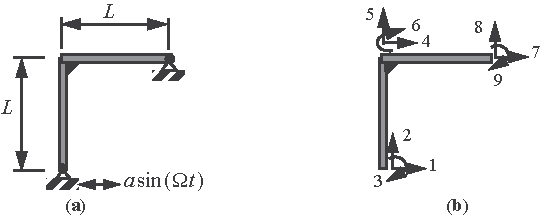
\includegraphics{Figure_18-21.pdf}
}{\caption{(a) Two-bar frame subject to harmonic excitation. (b) Degree of freedom numbering.\label{fig18.21}}}}

\vspace*{-1.6pc}

\begin{align}\label{ex18.5a}
\left\{u_{\alpha}(t)\right\}=\left[u_{3}(t)\enskip u_{4}(t)\enskip u_{5}(t)\enskip u_{6}(t)\enskip u_{9}(t)\right]^{T}.
\end{align}
The prescribed displacement vector is
\begin{align}\label{ex18.5b}
\left\{u_{\beta}(t)\right\}=\left[u_{1}(t)\enskip u_{2}(t)\enskip u_{7}(t)\enskip u_{8}(t)\right]^{T}=[a \sin (\Omega t)\enskip 0\enskip 0\enskip 0]^{T}.
\end{align}
The mass and stiffness matrices for element $\Omega_1$ are
\begin{align}\label{ex18.5c}
&\left[M^{(1)}\right]=\frac{m L}{420}
\begin{array}{@{}l@{}}
{\begin{array}{@{}l@{}}
\hspace*{10pt}\ddot{u}_1 \hspace*{15pt}\ddot{u}_2 \hspace*{15pt}\ddot{u}_3 \hspace*{15pt}\ddot{u}_4 \hspace*{15pt}\ddot{u}_5 \hspace*{15pt}\ddot{u}_6
\end{array}}\\
\left[\begin{array}{@{}cccccc@{}}156 & 0 & 44 & 54 & 0 & -26 \\0 & 140 & 0 & 0 & 70 & 0 \\44 & 0 & 16 & 26 & 0 & -12 \\54 & 0 & 26 & 156 & 0 & -44 \\0 & 70 & 0 & 0 & 140 & 0 \\-26 & 0 & -12 & -44 & 0 & 16\end{array}\right]\end{array}\nonumber\\
&\left[K^{(1)}\right]=\frac{E I_{x x}}{L^{3}}
\begin{array}{@{}l@{}}
{\begin{array}{@{}l@{}}
\hspace*{8pt}u_1 \hspace*{30pt}u_2 \hspace*{28pt}u_3 \hspace*{20pt}u_4 \hspace*{30pt}u_5 \hspace*{30pt}u_6
\end{array}}\\
\left[\begin{array}{@{}cccccc@{}}12 & 0 & 6 L & -12 & 0 & 6 L \\0 & \left(L/r_{x}\right)^{2} & 0 & 0 & -\left(L/ r_{x}\right)^{2} & 0 \\6 L & 0 & 4 L^{2} & -6 L & 0 & 2 L^{2} \\-12 & 0 & -6 L & 12 & 0 & -6 L \\0 & -\left(L/ r_{x}\right)^{2} & 0 & 0 & \left(L/r_{x}\right)^{2} & 0 \\6 L & 0 & 2 L^{2} & -6 L & 0 & 4 L^{2}\end{array}\right]\end{array}.
\end{align}
For element $\Omega_2$ the mass matrix is given by eq.~(\ref{eq18.186}), and the stiffness matrix is given by eq.~(\ref{eq18.187}), where the order of the columns is associated with generalized displacements $\left[\begin{array}{@{}llllll@{}}u_{4} & u_{5} & u_{6} & u_{7} & u_{8} & u_{9}\end{array}\right]$. Assemble the mass matrices to get the 9X9 unrestrained mass matrix $\left[M_{u}\right]=\left[M^{1)}\right]+\left[M^{(2)}\right]$ with due regard in the summation of the matrix elements from the individual mass matrices to their location in $\left[M_{u}\right]$. Similarly, the 9X9 unrestrained stiffness matrix is assembled as $\left[K_{u}\right]=\left[K^{(1)}\right]+\left[K^{(2)}\right]$. After assembly, the unrestrained matrix equation of motion is reordered by simultaneously interchanging the rows and columns to $\left[\begin{array}{@{}lllllllll@{}}u_{3} & u_{4} & u_{5} & u_{6} & u_{9} & u_{1} & u_{2} & u_{7} & u_{8}\end{array}\right]$.\vadjust{\pagebreak} The resulting matrix equation of motion in partitioned form is
\begin{align}\label{ex18.5d}
\left[\begin{array}{@{}l@{}}{\left[M_{\alpha \alpha}\right]\left[M_{\alpha \beta}\right]} \\{\left[M_{\beta \alpha}\right]\left[M_{\beta \beta}\right]}\end{array}\right]\left[\begin{array}{@{}l@{}}\left\{\ddot{u}_{\alpha}\right\} \\\left.\ddot{u}_{\beta}\right\}\end{array}\right]+\left[\begin{array}{@{}l@{}}{\left[K_{\alpha \alpha}\right]\left[\begin{array}{@{}l@{}}K_{\alpha \beta}\end{array}\right]} \\{\left[K_{\beta \alpha}\right]\left[\begin{array}{@{}l@{}}K_{\beta \beta}\end{array}\right]}\end{array}\right]\left[\begin{array}{@{}l@{}}\left\{u_{\alpha}\right\} \\\left\{u_{\beta}\right\}\end{array}\right]=\left[\begin{array}{@{}l@{}}\left\{Q_{\alpha}\right\} \\\left\{Q_{\beta}\right\}\end{array}\right].
\end{align}
The submatrices are
\begin{gather}
\left[M_{\alpha \alpha}\right]=\frac{m L}{420}\left[\begin{array}{@{}ccccc@{}}16 & 26 & 0 & -12 & 0 \\26 & 296 & 0 & -44 & 0 \\-12 & -44 & -44 & 32 & -12 \\0 & 0 & 26 & -12 & 16 \\0 & 0 & 26 & -12 & 16\end{array}\right]
\quad\left[M_{\alpha \beta}\right]=\frac{m L}{420}\left[\begin{array}{@{}cccc@{}}44 & 0 & 0 & 0 \\54 & 0 & 70 & 0 \\0 & 70 & 0 & 54 \\-26 & 0 & 0 & -26 \\0 & 0 & 0 & 44\end{array}\right]=\left[M_{\beta \alpha}\right]^{T}\label{ex18.5e}\\
\left[M_{\beta \beta}\right]=\frac{m L}{420}\left[\begin{array}{@{}cccc@{}}
156 & 0 & 0 & 0 \\
0 & 140 & 0 & 0 \\
0 & 0 & 140 & 0 \\
0 & 0 & 0 & 156 \\
\end{array}\right]
\quad\left[K_{\alpha \alpha}\right]
=\frac{EI_{xx}}{L^3}\left[\begin{array}{@{}ccccc@{}}
4L^2 & -6L & 0 & 2L^2  & 0\\
-6L & 12+(L/r_x)^2 & 0 & -6L & 0\\
0 & 0 & 12+(L/r_x)^2 & -6L & -6L \\
2L^2 & -6L & -6L & 8L^2 & 2L^2 \\
0 & 0 & -6L & 2L^2 & 4L^2\end{array}\right]\label{ex18.5f}\\
\left[K_{\alpha \beta}\right]=\frac{E I_{x x}}{L^{3}}\left[\begin{array}{@{}ccccc@{}}6 L & 0 & 0 & 0 \\-12 & 0 & -\left(L/ r_{x}\right)^{2} & 0 \\0 & -\left(L/r_{x}\right)^{2} & 0 & 12 \\6 L & 0 & 0 & 6 L \\0 & 0 & 0 & 6 L\end{array}\right]=\left[K_{\beta \alpha}\right]^{T} \quad\left[K_{\beta \beta}\right]=\frac{E I_{x x}}{L^{3}}\left[\begin{array}{@{}cccc@{}}12 & 0 & 0 & 0 \\0 & \left(L/r_{x}\right)^{2} & 0 & 0 \\0 & 0 & \left(L/ r_{x}\right)^{2} & 0 \\0 & 0 & 0 & 12\end{array}\right]\label{ex18.5g}\\
\left\{Q_{\alpha}\right\}=0_{5 X 1} \quad\left\{Q_{\beta}\right\}=\left[Q_{1}\quad Q_{2}\quad Q_{7}\quad Q_{9}\right]^{T}.\label{ex18.5h}
\end{gather}
There are no generalized forces prescribed in degrees of freedom 3, 4, 5, 6, and 9. The unknown generalized reaction force vector $\left\{Q_{\beta}\right\}$ corresponds to the prescribed generalized displacement vector $\left\{u_{\beta}\right\}$. The matrix equation of motion for the unknown generalized displacements is
\begin{align*}
\left[M_{\alpha \alpha}\right]\left\{\ddot{u}_{\alpha}\right\}+\left[M_{\alpha \beta}\right]\left\{\ddot{u}_{\beta}\right\}+\left[K_{\alpha \alpha}\right]\left\{u_{\alpha}\right\}+\left[K_{\alpha \beta}\right]\left\{u_{\beta}\right\}=0_{5 X 1}.
\end{align*}

\vspace*{-1pc}

Numerical data are taken from example~\ref{ex6.5} on page \pageref{ex6.5}: $a=0.03812\,\mathrm{m}$, $A=171.014 \times 10^{-6}\,\mathrm{m}^{2}$, $I_{x x}=124.25 \times 10^{-9}\,\mathrm{m}^{4}$, $L=0.8\,\mathrm{m}$, $r_{x}=0.0269546\,\mathrm{m}$, $E=68.3 \times 10^{9}\,\mathrm{N}/\mathrm{m}^{2}$, $\rho=2{,}710\,\mathrm{Kg}/ \mathrm{m}^{3}$, and $m=\rho A=0.463448\,\mathrm{Kg}/\mathrm{m}$. The eigenvalue problem for the free vibrations of the frame is
\begin{align}\label{ex18.5i}
\left[K_{\alpha \alpha}\right]\{\phi\}-\lambda\left[M_{\alpha \alpha}\right]\{\phi\}=0_{5 X 1}.
\end{align}
The numerical results for the eigenvalues and corresponding eigen vectors are
\begin{gather}
\left(\lambda_{1},\left\{\phi_{1}\right\}\right)=\left(9.99471 \times 10^{7},\left[\begin{array}{@{}c@{}}0.324108 \\0.268035 \\0.268035 \\0.324108\end{array}\right]\right)
\quad\left(\lambda_{2},\left\{\phi_{2}\right\}\right)=\left(6.783 \times 10^{7},\left[\begin{array}{@{}c@{}}-1 \\0.595335 \\-0.595335 \\-1.026 \times 10^{-15} \\1\end{array}\right]\right)\label{ex18.5j}\\
\left(\lambda_{3},\left\{\phi_{3}\right\}\right)=\left(1.78362 \times 10^{7},\left[\begin{array}{@{}c@{}}1 \\ -0.105789 \\ -0.105789 \\ 0.972216\\
1\end{array}\right]\right)
\quad\left(\lambda_{4},\left\{\phi_{4}\right\}\right)=\left(2.89664 \times 10^{6},\left[\begin{array}{@{}c@{}}1 \\0.0104001 \\-0.0104001 \\-2.72413 \times 10^{-15} \\ -1\end{array}\right]\right)\label{ex18.5k}\\
\left(\lambda_{5},\left\{\phi_{5}\right\}\right)=\left(854,421,\left[\begin{array}{@{}c@{}}1 \\0.00365009 \\0.00365009 \\-0.991238 \\1\end{array}\right]\right).\label{ex18.5l}
\end{gather}
The natural frequencies are given by $\omega_{i}=\sqrt{\lambda_{i}}$, $i=1,2, \ldots, 5$.
\begin{align}\label{ex18.5m}
\left[\begin{array}{@{}lllll@{}}\omega_{1} & \omega_{2} & \omega_{3} & \omega_{4} & \omega_{5}\end{array}\right]=\left[\begin{array}{@{}lllll@{}}9,997.36 & 8,235.9 & 4,223.3 & 1,701.95 & 924.346\end{array}\right] \mathrm{rad}/\mathrm{s}.
\end{align}
The prescribed displacement terms in the matrix equation of motion lead to a generalized force vector defined by
\begin{align}\label{ex18.5n}
\left\{\bar{Q}_{\alpha}\right\}=-\left[M_{\alpha \beta}\right]\left\{\ddot{u}_{\beta}\right\}-\left[K_{\alpha \beta}\right]\left\{u_{\beta}\right\}.
\end{align}
Numerical evaluation of this generalized force vector is
\begin{align}\label{ex18.5o}
\left\{\bar{Q}_{\alpha}\right\}=\left[\begin{array}{@{}c@{}}-3,032.78+0.00148063 \Omega^{2} \\7,581.96+0.00181714 \Omega^{2} \\0 \\-3,032.78-0.000874919 \Omega^{2} \\0\end{array}\right] \sin \Omega t.
\end{align}
The matrix equation of motion governing the unknown displacements is rewritten as
\begin{align}\label{ex18.5p}
\left[M_{\alpha \alpha}\right]\left\{\ddot{u}_{\alpha}\right\}+\left[K_{\alpha \alpha}\right]\left\{u_{\alpha}\right\}=\left\{\bar{Q}_{\alpha}\right\}.
\end{align}
The initial conditions are $\left\{u_{\alpha}(0)\right\}=0_{5 X 1}$ and $\left\{\dot{u}_{\alpha}(0)\right\}=0_{5 X 1}$. Transform from the physical displacements to the modal displacements by $\left\{u_{\alpha}(t)\right\}=[\Phi]\{q(t)\}$, where the columns of the modal matrix $[\Phi]$ are the eigenvectors. Equations of motion in modal coordinates are
\begin{align}\label{ex18.5q}
\left[M_{g}\right] \ddot{q}+\left[K_{g}\right]\{q\}=\left\{F_{g}(t)\right\},
\end{align}
where the generalized mass, stiffness, and force vector are
\begin{gather}
\left[M_{g}\right] =\operatorname{diag}\left[\begin{array}{@{}lllll@{}}0.02135 & 0.140492 & 0.0144387 & 0.0292596 & 0.098909\end{array}\right]\label{ex18.5r}\\
\left[K_{g}\right] =\operatorname{diag}\left[\begin{array}{@{}lllll@{}}2134.77 & 9529.59 & 257.532 & 84.7545 & 84.5099\end{array}\right] 10^{3},\nonumber\\
\left\{F_{g}(t)\right\}=\{A(\Omega)\} \sin \Omega t,\ \text{and where}\label{ex18.5s}\\
\{A(\Omega)\}=\left[\begin{array}{@{}c@{}}-1,983.5+92.0225 \times 10^{-6} \Omega^{2} \\7,275.15-463.879 \times 10^{-6} \Omega^{2} \\
-6{,}061.51+610.799 \times 10^{-6} \Omega^{2} \\
-2{,}953.93+1,499.53 \times 10^{-6} \Omega^{2} \\
1.10169+2{,}354.52 \times 10^{-6} \Omega^{2}
\end{array}\right].\label{ex18.5t}
\end{gather}
The equation of motion for each modal coordinate is in the form
\begin{align}\label{ex18.5u}
\ddot{q}_{i}+\omega_{i}^{2} q_{i}=\frac{1}{M_{g}(i, i)} A_{i}(\Omega) \sin (\Omega t) \quad i=1,~2, \ldots, 5,
\end{align}
subject to initial conditions $q_{i}(0)=0,\text{ and }\dot{q}_{i}(0)=0$. The solution for $\Omega \neq \omega_{i}$ is
\begin{align}\label{ex18.5v}
q_{i}(t)=\frac{A_{i}(\Omega)}{M_{g}(i, i)\left(\omega_{i}^{2}-\Omega^{2}\right)}\left[\frac{-\Omega}{\omega_{i}} \sin \left(\omega_{i} t\right)+\sin (\Omega t)\right].
\end{align}
The solution for $\Omega=\omega_{i}$ is
\begin{align}\label{ex18.5w}
q_{i}(t)=\frac{-A_{i}\left(\omega_{i}\right)}{2 M_{g}(i, i) \omega_{i}^{2}}\left[\left(\omega_{i} t\right) \cos \left(\omega_{i} t\right)-\sin \left(\omega_{i} t\right)\right].
\end{align}
Transform from modal coordinates to physical coordinates by $\left\{u_{\alpha}(t)\right\}=[\Phi]\{q(t)\}$. The vertical displacement at the joint connecting the frame members is $u_{5}(t)$, and for $\Omega=0.9 \omega_{1}$ it is
\begin{align}\label{ex18.5x}
u_{5}(t)=\ &256.346 \times 10^{-6} \sin (\Omega t)-333.609 \times 10^{-6} \sin \left(\omega_{5} t\right)-151.009 \times 10^{-6} \sin \left(\omega_{4} t\right)\nonumber\\
&-47.4688 \times 10^{-6} \sin \left(\omega_{3} t\right)+ 41.6693 \times 10^{-6} \sin \left(\omega_{2} t\right)+20.1981 \times 10^{-6} \sin \left(\omega_{1} t\right).
\end{align}
{\def\thefigure{18.22}
\processfigure[b]{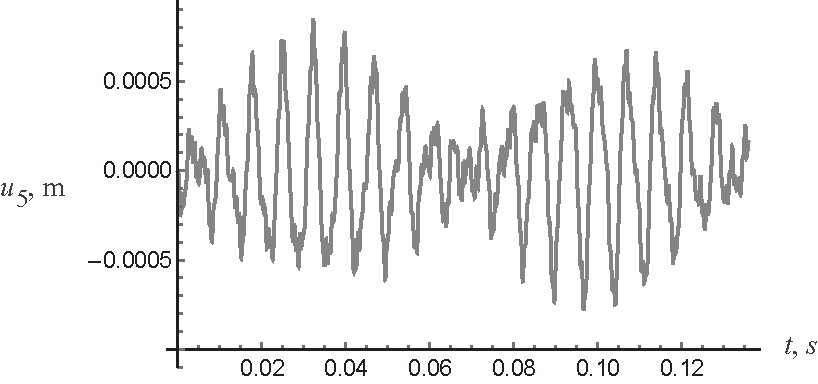
\includegraphics{Figure_18-22.pdf}
}{\caption{Response of $u_5(t)$ for $\Omega = 0.90 \omega_5$.\label{fig18.22}}}}
The first term on the right-hand side of $u_{5}(t)$ is the forced motion and has the same frequency as the excitation. The remaining five terms on the right-hand side constitute the natural motion with contributions from the five natural frequencies of the frame. A graph of the displacement response is shown in figure~\ref{fig18.9} for $0 \leq t \leq 20 \tau$, where $\tau$ is the period of the lowest natural frequency (i.e., $\tau=(2 \pi)/\omega_{5}=0.006797\,\mathrm{s}$). The displacement response exhibits the phenomena of \textit{beating}.
\begin{quote}
 Pure undamped beating, in general, is the combination of two sinusoids that have different but closely spaced frequencies, as the two sinusoids pass into and out of phase with each other. (Hallauer, 2016).
\end{quote}
In the case of the frame response shown in figure~\ref{fig18.22}, the driving frequency $\Omega$ is close to the lowest natural frequency $\omega_{5}$, and it is the combination of the two sinusoids $\sin (\Omega t)$ and $\sin \left(\omega_{5} t\right)$ that are the source of beating.

For $\Omega=\omega_{5}$, the displacement $u_{5}(t)$ is
\begin{align}\label{ex18.5y}
u_{5}(t)=&-0.406236 t \cos (\Omega t)+319.34 \times 10^{-6} \sin \left(\omega_{5} t\right)-158.115 \times 10^{-6} \sin \left(\omega_{4} t\right)\nonumber\\
&-52.3109 \times 10^{-6} \sin \left(\omega_{3} t\right)+ 45.9088 \times 10^{-6} \sin \left(\omega_{2} t\right)+22.3042 \times 10^{-6} \sin \left(\omega_{1} t\right).
\end{align}
{\def\thefigure{18.23}
\processfigure{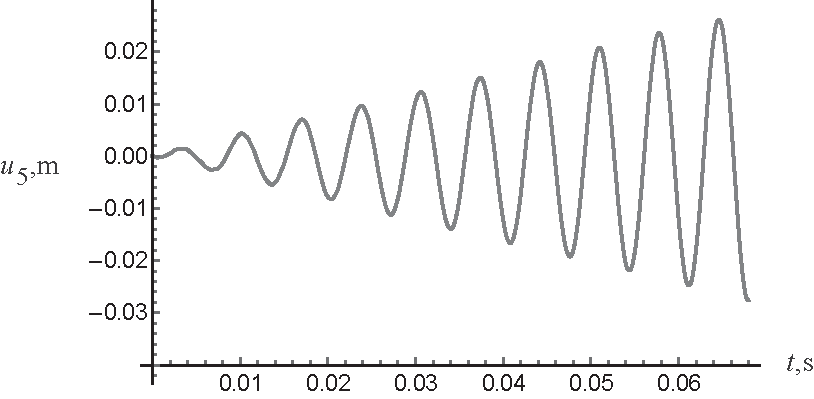
\includegraphics{Figure_18-23.pdf}
}{\caption{Response of $u_5(t)$ for $\Omega = \omega_5$.\label{fig18.23}}}}
\noindent A graph of the displacement response is shown in figure~\ref{fig18.23} for $0 \leq t \leq 10 \tau$, where $\tau$ is the period of the lowest natural frequency. As shown in the graph, the amplitude of the vibrations for $\Omega=\omega_{5}$ increase linearly in time, which is the condition of \textit{resonance}.
\end{example}

\vspace*{-1pc}

\begin{thebibliography}{}\label{sec18.10}
\bibitem{}
Bathe, K-L. \textit{\textbf{Finite Element Procedures in Engineering Analysis}}. Englewood Cliffs, NJ: Prentice-Hall Inc., 1982.\label{Bathe}

\bibitem{}
Boresi, A. P. \textit{\textbf{Elasticity In Engineering Mechanics}}. Englewood Cliffs, N.J: Prentice-Hall, Inc. 1965, p. 34.

\bibitem{}
Craig, Roy R., Jr. \textit{\textbf{Structural Dynamics}:} \textit{\textbf{An Introduction to Computer Methods}}. New York: John Wiley \& Sons, Inc., 1981, pp. 212--217, 321--340, 455--464.\label{Craig}

\bibitem{}
Hallauer, W. L., Jr., \textit{\textbf{Introduction to} \textbf{Linear}, \textbf{Time-Invarian}t, \textbf{Dynamic Systems} \textbf{for} \textbf{Students of Engineering}.} Blacksburg, VA: Self-published, 2016. \url{http://hdl.handle.net/10919/78864.}

\bibitem{}
Isakowitz, Steven J. \textit{\textbf{Space Launch Systems}}, 2d ed. Updated by Jeff Samella.Washington DC: American Institute of Aeronautics and Astronautics, 1995, pp. 201--218.

\bibitem{}
Langhaar, H. L. \textit{\textbf{Energy Methods in Applied Mechanics}}. New York: John Wiley, and Sons, Inc., 1962.\label{Langhaar}

\bibitem{}
Qu, Zu-Qing. \textit{\textbf{Model Order Reduction Techniques, With Application to Finite Element Analysis}}. London: Springer-Verlag, 2004.\label{Qu2004}

\bibitem{}
Sarafin, Thomas, P., ed. \textit{\textbf{Spacecraft Structures and Mechanisms – From Concept to Launch}}. Torrance, CA, and Dordrecht, The Netherlands: Microcosom Press, and Kluwer, 1995, pp. 49 \& 50.\label{Sarafin1995}

\bibitem{}
Schiesser, W. E. \textit{\textbf{Computational Mathematics in Engineering and Applied Science}}. Boca Raton, FL: CRC Press, 1994, Chapter 2.

\bibitem{}
Szabó, B., and I. Babuska. \textit{\textbf{Finite Element Analysis}}. New York: John Wiley \& Sons, 1991, pp. 163--166.
\end{thebibliography}

\pagebreak

\section{Practice exercises}\label{sec18.11}

\setcounter{equation}{195}

\begin{exercise}
\begin{enumerate}[\textbf{2.}]
\item[\textbf{1.}]
The Lagrangian for a three-degree-of-freedom model of Atlas I is
\begin{align}\label{eq18.196}
L=\frac{m_{1}}{6}\left[\left(\dot{w}_{1}\right)^{2}+\dot{w}_{1} \dot{w}_{2}+\left(\dot{w}_{2}\right)^{2}\right]+\frac{1}{2} m_{2}\left(\dot{w}_{2}\right)^{2}+\frac{1}{2} m_{3}\left(\dot{w}_{3}\right)^{2}-\frac{1}{2} k_{12}\left(w_{1}-w_{2}\right)^{2}-\frac{1}{2} k_{23}\left(w_{3}-w_{2}\right)^{2},
\end{align}
where $w_{1}(t)$ is the displacement at the bottom of the booster, $w_{2}(t)$ is the displacement at the top of Centaur, and $w_{3}(t)$ is the displacement of the payload. These displacements are defined with respect to the equilibrium state. The combined mass of the booster and Centaur is denoted by $m_1$, the mass of the fairing by $m_2$, and the mass of the payload by $m_3$. Masses are determined from the weight data given in ``Description of Atlas I'' on page \pageref{sec18.1}. The spring stiffness $k_{12}$ and $k_{23}$ are listed in ``Step 1: Equations of motion about equilibrium.'' on page \pageref{step1}. Lagrange's equations of motion are
\begin{align}\label{eq18.197}
\frac{d}{d t}\left(\frac{\partial L}{\partial \dot{w}_{1}}\right)-\frac{\partial L}{\partial w_{1}}=R_{1} \quad \frac{d}{d t}\left(\frac{\partial L}{\partial \dot{w}_{2}}\right)-\frac{\partial L}{\partial w_{2}}=0 \quad \frac{d}{d t}\left(\frac{\partial L}{\partial \dot{w}_{3}}\right)-\frac{\partial L}{\partial w_{3}}=0,
\end{align}
where ${R}_1 = 77,100$. lb is the net thrust. Determine the maximum payload load factor during the initial instants of lift off. Partial answer: the value and its associated eigenvector for the smallest elastic mode is
\begin{align}\label{eq18.198}
\left(\lambda_{2},\left\{\phi_{2}\right\}\right)=\left(15,710.5,\left[\begin{array}{@{}c@{}}-0.795164 \\0.760969 \\1\end{array}\right]\right).
\end{align}
The eigenvector is normalized such that the magnitude of its largest component is a positive one.

\item[\textbf{2.}] Determine the natural frequencies in Hz and the corresponding modal vectors for the five-bar, pin-jointed truss shown in figure~\ref{fig18.24}. Normalize the modal vectors such that the largest component in the vector is a positive 1. Sketch the mode shapes.\vspace*{-12pt}

    {\def\thefigure{18.24}
\processfigure{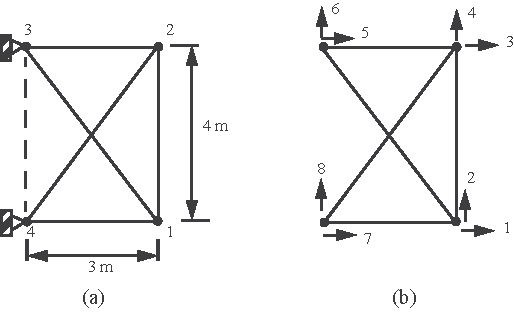
\includegraphics{Figure_18-24.pdf}
}{\caption{(a) Five-bar truss,
(b) Degrees of freedom.\label{fig18.24}}}}

\vspace*{-1pc}

\item[\textbf{3.}] The three-bar truss in example~\ref{ex18.3} on page \pageref{ex18.3} is subjected to the following initial conditions
\begin{align}\label{eq18.199}
\left[\begin{matrix}u_{1}(0) \\u_{2}(0)\end{matrix}\right]=
\left.\left[\begin{matrix}0 \\0\end{matrix}\right] \quad\left[\begin{matrix}\displaystyle\frac{d u_{1}}{d t} \\[8pt] \displaystyle\frac{d u_{2}}{d t}\end{matrix}\right]\right|_{t=0}=
\left[\begin{matrix}0 \\1\end{matrix}\right] \mathrm{m}/\mathrm{s}.
\end{align}

\begin{enumerate}[b)]
  \item[{\hskip13pt}a)] Determine the generalized mass matrix $\left[M_{g}\right]$, the generalized stiffness matrix $\left[K_{g}\right]$, and the initial\break\hspace*{34pt} conditions in modal coordinates (begin with eqs. (\textbf{d}) and (\textbf{e})).
  \item[{\hskip13pt}b)] Determine the solution in modal coordinates and in physical coordinates.
  \item[{\hskip13pt}c)] Determine the transient bar forces $N_{1-2}(t), N_{1-3}(t), \text{and } N_{1-4}(t)$.
  \item[{\hskip13pt}d)] Plot the bar forces found in part (c) for $0 \leq t \leq 0.015\,\mathrm{s}$.
\end{enumerate}

\item[\textbf{4.}] Model the cantilever beam in example~\ref{ex18.4} on page \pageref{ex18.4} with two equal length elements as shown in figure~\ref{fig18.25}.

{\def\thefigure{18.25}
\processfigure{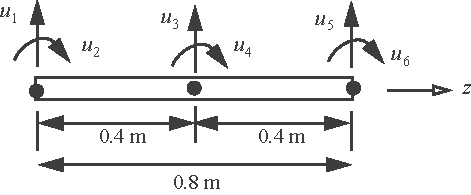
\includegraphics{Figure_18-25.pdf}
}{\caption{Beam of example \ref{ex18.4} modeled with two elements.\label{fig18.25}}}}

\vspace*{-1pc}



\begin{enumerate}[b)]
  \item[{\hskip13pt}a)] Determine the natural frequencies in Hz and the corresponding modal vectors. Normalize the modal\break\hspace*{34pt} vectors such that the tip displacement $u_5$ is equal to one in each mode. Refer to table~\ref{tab18.4}.
  \item[{\hskip13pt}b)] Determine the percentage error of each frequency with respect to the exact frequency from the continuous\break\hspace*{34pt} beam vibration analysis.

  \item[{\hskip13pt}c)] Plot the lateral displacement of the beam, $0 \leq z \leq 0.8\,\mathrm{m}$, for each mode using eq.~(\ref{eq17.69}) on page \pageref{eq17.69}\break\hspace*{34pt} and matrix $\left[G_{a q}\right]$ from the last three rows of eq.~(\ref{eq18.162}).
\end{enumerate}\enlargethispage{2\baselineskip}

%\begin{minipage}{290pt}
\item[\textbf{5.}] The uniform beam shown in figure~\ref{fig18.26} is simply supported at each end. The material and geometric properties are the same as those given in example~\ref{ex18.4},

{\def\thefigure{18.26}
\processfigure{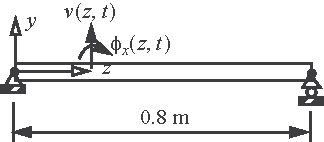
\includegraphics{Figure_18-26.pdf}
}{\caption{Simply supported beam. \label{fig18.26}}}}

\begin{enumerate}[b)]
  \item[{\hskip13pt}a.] Determine the first two natural frequencies in Hz for the beam modeled with \textbf{one} element. Use the\break\hspace*{33pt} condensed mass matrix (\ref{eq18.167}) and stiffness matrix (\ref{eq17.106}) on page \pageref{eq17.106}.
  \item[{\hskip13pt}b.] Compute the percent discrepancy of the frequencies with respect to the continuous beam solution. The\break\hspace*{30pt} frequencies for the continuous beam vibration analysis in rad/s are listed in Graig (1981) as\break\hspace*{34pt} $\omega_{n}=\left(\frac{n \pi}{l}\right)^{2} \sqrt{\frac{E I_{x x}}{\rho A}}$ \quad $n=1,2$.
\end{enumerate}
%\end{minipage}

\end{enumerate}
\end{exercise}



\clearemptydoublepage


\end{document} 